%!TEX TS-program = pdflatexmk
%\documentclass[12pt,a4paper,UKenglish]{article}
\documentclass[UKenglish]{ifimaster}  % added
\usepackage[utf8]{inputenc}
\usepackage[T1]{fontenc, url}
\urlstyle{sf}
\usepackage{float}
\usepackage{graphicx, epstopdf}
\usepackage{subfig}
\usepackage{multirow}
\usepackage{siunitx}
\usepackage{babel,csquotes,newcent,textcomp,ifimasterforside,varioref}
%\usepackage{babel,csquotes,newcent,textcomp} %my
\usepackage[backend=biber, sortcites, sorting=none ]{biblatex} %my
%\usepackage[backend=biber,style=numeric-comp]{biblatex}
%\usepackage{subfig} %my
\usepackage{hyperref}
%\hypersetup{colorlinks=true, linktoc=none, linkcolor=blue,} %my
\hypersetup{pageanchor=false,colorlinks=true, linktoc=all, linkcolor=blue,}
\usepackage [nopostdot, acronym, nogroupskip, nonumberlist,] {glossaries}
\usepackage{wrapfig}

%fancy header and footer
\usepackage{fancyhdr}
\setlength{\headheight}{15pt}
\pagestyle{fancy}
\renewcommand{\chaptermark}[1]{ \markboth{#1}{} }
\renewcommand{\sectionmark}[1]{ \markright{#1} }
\fancyhf{}
\fancyfoot[LE,RO]{\thepage}
\fancyhead[LE]{\textbf{ \nouppercase{\leftmark}} }
\fancyhead[RO]{\textbf{ \nouppercase{\leftmark}} }
\fancypagestyle{plain}{ %
  \fancyhf{} % remove everything
  \renewcommand{\headrulewidth}{0pt} % remove lines as well
  \renewcommand{\footrulewidth}{0pt}}

\setacronymstyle{long-short}
\glsdisablehyper

\makenoidxglossaries

\newacronym{ldo}{LDO}{linear dropout}
\newacronym{pcb}{PCB}{printed circuit board}
\newacronym{mos}{MOS}{metal-oxide-semiconductor}
\newacronym{nmos}{nMOS}{n-channel MOS}
\newacronym{pmos}{pMOS}{p-channel MOS}
\newacronym{cmos}{CMOS}{complementary metal-oxide-semiconductor}
\newacronym{vpp}{Vpp}{peak to peak voltage}
\newacronym{vp}{Vp}{peak voltage}
\newacronym{vce}{VCE}{voltage conversion efficiency}
\newacronym{pce}{PCE}{power conversion efficiency}
\newacronym{vtn}{Vtn}{thresold voltage of n-channel MOS}
\newacronym{vtp}{Vtp}{thresold voltage of p-channel MOS}
\newacronym{smps}{SMPS}{switch mode power supply}
\newacronym{pssr}{PSSR}{power supply rejection ratio}
\newacronym{icmr}{ICMR}{input common mode range}
\newacronym{dc}{DC}{direct current}
\newacronym{pm}{PM}{phase margin}
\newacronym{gm}{GM}{gain margin}
\newacronym{esr}{ESR}{equivalent series resistance}
\newacronym{ugf}{UGF}{unity gain frequency}
\newacronym{pvt}{PVT}{process voltage temperature}
\newacronym{ptat}{PTAT}{proportional to absolute temperature}
\newacronym{ctat}{CTAT}{complementary to absolute temperature}
\newacronym{tc}{TC}{temperature coefficient}
\newacronym{bgr}{BGR}{bandgap reference}
\newacronym{ota}{OTA}{operational transconductance amplifier}
\newacronym{bjt}{BJT}{bipolar junction transistor}
\newacronym{pnp}{PNP}{BJT where n-type semiconductor is between two p-type semiconductors}
\newacronym{pms}{PMS}{Power Management System}
\newacronym{smd}{SMD}{Surface Mounted Device}
\newacronym{srf}{SRF}{self resonance frequency}

\newacronym{wpt}{WPT}{Wireless Power Transfer}
\newacronym{ipt}{IPT}{Inductive Power Transfer}
\newacronym{pru}{PRU}{Power Receiving Unit}
\newacronym{ptu}{PTU}{Power Transfer Unit}
\newacronym{jlcc}{JLCC}{J-Lead Chip Carrier}
\newacronym{mlcc}{MLCC}{Multi-Layer Ceramic Capacitor}
\newacronym{nordic}{NORDIC}{Nordic Semiconductor}
\newacronym{soc}{SOC}{System on a Chip}
\newacronym{rfid}{RFID}{Radio Frequency Identification}
\newacronym{rf}{RF}{Radio Frequency}
\newacronym{ism}{ISM}{Industrial, Scientific and Medical }
%\newacronym{fcc}{FFC}{Federal Communications Commission}
\newacronym{fcc}{FCC}{Federal Communications Commission}
\newacronym{ieee}{IEEE}{ Institute of Electrical and Electronics Engineers}


% *********************************************************************** COVER ABSTRACT PREFACE  ***********************************************************************

%\title{Preliminary report on master project}
%\author{Rikesh Chauhan}
%\date{}
\title{Wireless Power Receiving Unit}        
\subtitle{Analysis, design and implementation of inductive power receiving unit for wireless circuits}         
\author{Rikesh Chauhan}         

%\addbibresource{preliminary.bib}
\bibliography{reference.bib}   

\begin{document}
\ififorside{}
\frontmatter{}
\maketitle{}

%\chapter*{Abstract}
%\chapter*{Preface} 
%HERE IS THE ABSTRACT
\tableofcontents{}
\listoffigures{}
\listoftables{}
                  
\mainmatter{}

% ************************************************************ INTRODUCTION AND BACKGROUND *************************************************************************

\part{Introduction and Background}

\chapter{Introduction}

\section{Motivation}

We start with the technology development trend in micorelectronics. The progress of different aspects of 
technology is discussed and compared with power/battery development. We end the chapter concluding the need for
going cordless for suppling power for microelectronics.
% The ongoing modern technological advancements have led us into dramatic and drastic electronic device development 
% trend.  On the one hand devices are getting smaller, lighter and low-powered, while on the other hand more and 
% more functionality with increased speed are being integrated. And above all these, going wireless whenever and 
% whatever possible is the market trend. Specially in commercial electronics, it looks like quest for the ultimate 
% gadget, miniaturised low-powered multi-functional wireless device, is not going to stop anytime soon. Thanks to 
% non-stop research and development in manufacturing, material and technology. \\


\subsection{Technology Trend}

\subsubsection{Size and Weight : Lighter and Tighter}

Reduction in size and weight has been most dramatic that in course of some decades miniaturisation trend went 
from a room-sized fixed electronic into a wearable device. Most important milestone contributing for lighter and 
tighter devices is development of transistor in 1950s replacing large and bulky vacuum tubes, and  
development first IC in 1965 making it possible to integrated hundreds of transistors on a single silicon substrate of 
some square mm. Since then as stated by Moorse's law, IC size is continuously shrinking. A typical modern IC now 
consists of billions of transistors of some  tens of nm feature size. \\

\begin{figure}[!htbp] %figure placement: here, top, bottom, or page
   \centering
   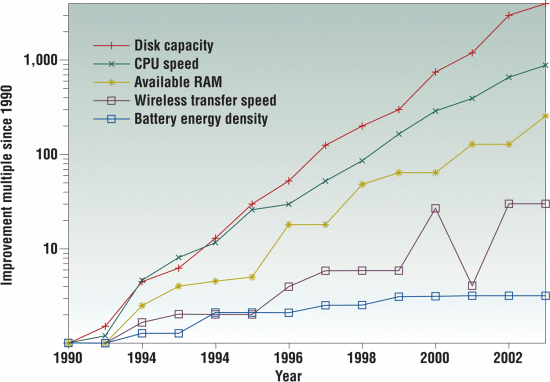
\includegraphics[width=0.9\textwidth]{img/comp_tech_batt.png}
   \caption{Mobile performance development trend \cite{mobile_performance}}
   \label{fig:comp_tech_batt}
\end{figure}

\subsubsection{Operation: Multi-functional and Higher speed}

On the contrary to shrinking device size, integrated functionality and device speed is increasing proportionally. 
The introduction of SoCs created of new dawn of multi-functionality IC by integrating many electronic components 
and/or systems on a single silicon substrate. Similarly multi-core CPU with parallel programmed instruction  
significantly increased work payload as stated by Amdahl's law. Similarly recent developments in IoT has 
introduced whole new dimension on multi-functionality by connecting many devices to a same local network or 
the internet\cite{iot_intro}. \\

\subsubsection{Power consumption: Low-power}

In terms of power consumption, though power density has increased due to increased transistor density and speed, 
power consumption per transistor and energy per operation, EOP, has significantly reduced. It is due to gradual 
shrinking in feature size and decrease in supply voltage. Similarly there has been a lot progress in LP design 
introducing new power optimal design techniques both at logic/circuit level and architecture level. Lately run 
time power optimisation technique by tracing realtime work load like dynamic voltage scaling and switching 
between different operation modes (sleep, nap, doze and active) have been popularly used to reduce power 
consumption\cite{rabaey_2009}. \\

%http://www.cisco.com/c/dam/en_us/solutions/trends/iot/introduction_to_IoT_november.pdf

\subsubsection{Power supply: Cut the Cord}

In spite of dramatic technological advancement, battery technology has not evolve equally as good, see figure 
\ref{fig:comp_tech_batt}. It is not like there has been no progress in battery technology at all. There has been a lot improvements 
like increased volumetric energy density thereby reducing size, increased gravimetric energy density thereby 
reducing weight, reduced self discharge thereby increasing life time and increased charged cycle thereby 
increasing reuse.[CITE]. Today Li-ion has better choice for powering devices because of it better combined 
above mentioned characteristics and hence used excessively in portable and wearable devices. \\

But use of battery in todays'  portable and wearable devices is constraining the overall development of devices 
[CITE]. Batteries contribute significant proportion of total weight and size of the device. They supply limited 
power which means require regular recharge and in the long run need replacement. During recharge either device or 
battery has to be physically connected to power outlet. \\

A power source with high power density which perpetually and wirelessly power devices could eliminate 
all the above problems and challenges mentioned above. But how 
far have we gone to achieve this? In the next chapter, we will discussed the techniques of energy harvesting and 
wireless power transfer studied and implemented so far. Bluetooth Low Energy, BLE is taken as a 
reference device to drive and a power harvesting circuit is designed and implememted for BLE. \\

% WPT helps to overcome some of these limitations. For example instead of removing and recharging batteries, 
% they can be recharged with 
% harvested energy without removing them. Going one step further ahead, batteries can be completely replaced in 
% a electronic device and power the device wirelessly. This way implementation of WPT helps to minimise the 
% problems of battery powered device and in the best case completely removes the problems. \\

\section{Thesis outline}

A brief overview of this thesis report is presented below. For better organisation and clarity of content, it is divided into four parts 
and eight chapters. 
\begin{itemize}
\item \textbf{Chapter 1} discusses the motivation behind this work. It compares technology trends and concludes
the need of going cordless power source for modern microelectronics devices.
\item \textbf{Chapter 2} presents the background for this work. It discusses various energy harvesting and 
wireless power transfer techniques.
\item \textbf{Chapter 3} onwards, design of functional blocks is discussed. It starts with design and 
and analysis of rectifier topology used.
\item \textbf{Chapter 4} is about design, implementation and analysis of LDO.
\item \textbf{Chapter 5} discusses about modelling the antenna required and its performance. 
\item \textbf{Chapter 6} presents design of wireless power harvesting system using the discrete functional blocks and simulation 
results are presented. First only the power management system is simulated and then compete power transfer system with 
inductive transfer link.
\item \textbf{Chapter 7} discusses the production, test and verification of produced power harvesting chip. First test PCB and 
chip layout is discussed. Then measurement data of the chip is presented and finally compared with the simulated results.
\item \textbf{Chapter 8} presents summary and concluding remarks of this work including problems and challenges faced 
along with prospective future work.

\end{itemize}




\chapter{Background}

\section{Energy Harvesting}

In this chapter, we discuss the options to elimanate or minimise the bottlenecks of battery used in portable and 
wearbale devices. We start with energy harvesting techniques and then wireless power transfer techniques. \\

There has been success in harvesting low power from ambient sources and a lot of effort and resources is being used for 
harvesting high power. As discussed earlier the technological advancement has given us low power electronics. 
These LP devices can now be powered solely by harvested energy, eventually making battery-less wirelessly powered 
electronic device a reality. \\

Energy harvesting system generally constitutes of energy source, transducer and power conditioning unit as shown 
in figure \ref{fig:visio_harvest_func}. Energy 
source can either be artificial like human walking or natural like sunlight. Transducer are devices which 
converts the energy from source which may be to electrical energy. And power conditioning unit process the 
harvested energy so that it can be used either to directly power a load or to store the energy. \\

\begin{figure}[!htbp] %figure placement: here, top, bottom, or page
   \centering
   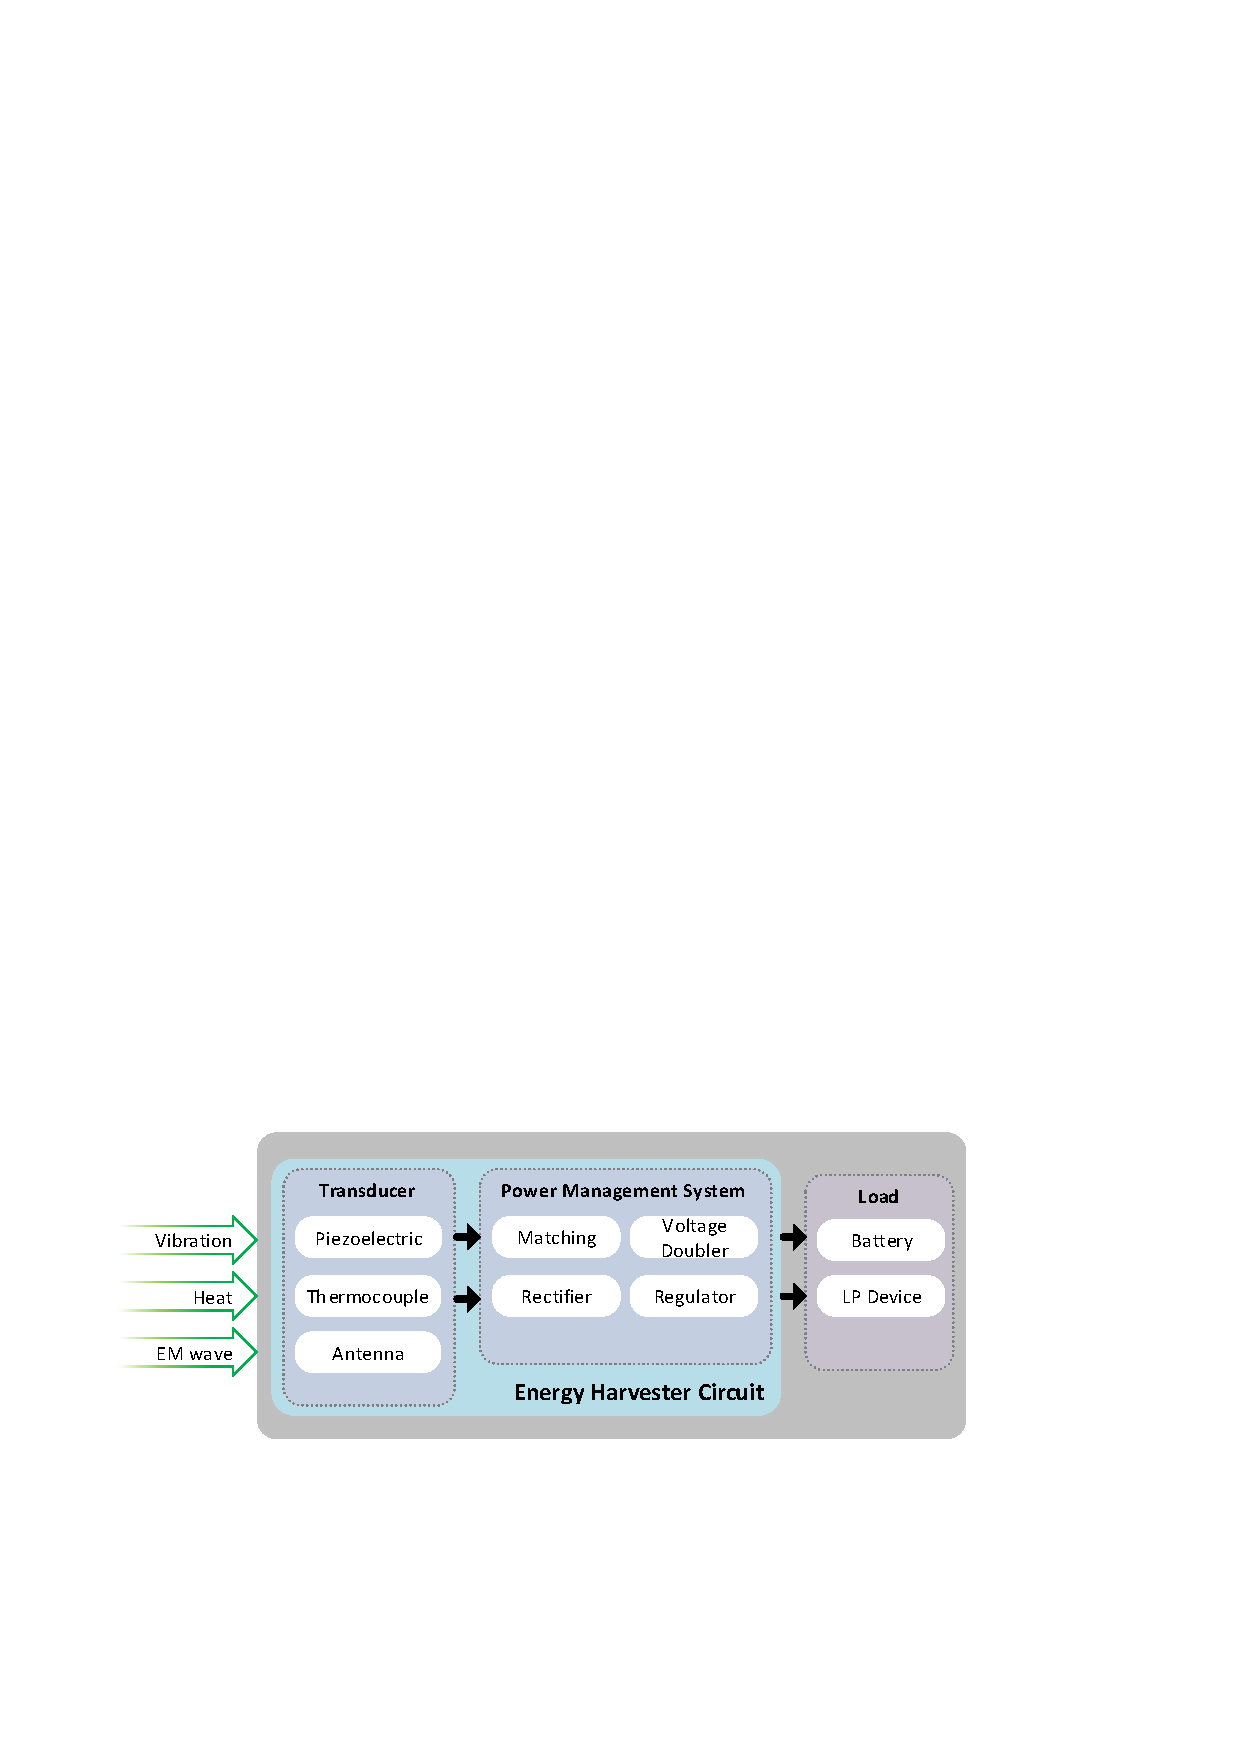
\includegraphics[width=\textwidth]{img/visio_harvest_func.pdf}
   \caption{Functional block diagram of energy harvesting system}
   \label{fig:visio_harvest_func}
\end{figure}


Depending upon the type of energy harvested from the surrounding environment, energy harvesting devices can be 
broadly classified into kinetic, electromagnetic and thermal energy sources\cite{review_energy_harvest}. These are 
briefly discussed below.\\

\subsection{Kinetic energy harvesting}
In kinetic energy harvesting, kinetic energy due to mechanical deformation of transducer is converted into 
electrical energy. Piezoelectrical material is good example of transducer for kinetic energy harvesting. 
Piezoelectrical materials are those which exhibit piezoelectric effect: when subjected to mechanical strain, 
it generates electrical charge proportional to applied strain. Strain is applied with either compression, slap 
or bending of the material. \\


\subsection{Harvesting from Radiation}
Electromagnetic energy harvesting is extraction of useful energy from ambient light or RF radiation. Solar energy 
harvesting is the most popular and widely successful EM energy harvesting for large scale energy generation. It 
makes use of semiconductor device called solar cells as transducer. These transducer converts incident light 
energy to electric energy due to photoelectric effect: when light is incident on semiconductor, electrons are 
emitted from the surface.  Its application ranges from LP wrist watch to grid of photovoltaic system. The other 
popular example is harvesting from  RF radiation, which are available almost everywhere in modern cities, to 
power RFIDs. In this technique, antenna or rectenna are used as transducer. However harvesting from RF radiation 
has been limited to very low power only. \\

\subsection{Thermal energy harvesting}
Similarly in thermal energy harvesting, thermal energy from any source in the environment is converted to useful 
electric energy. Thermopile is an example of thermal energy harvesting using thermocouples in series as 
transducer. Thermocouple is a electric device with two different conductors forming junctions. A thermocouple 
generates voltage proportional to temperature between junctions, known as Seeback effect. Connecting 
thermocouples in series increased the harvested voltage as in thermopile. \\

\begin{figure}[H] %figure placement: here, top, bottom, or page
   \centering
   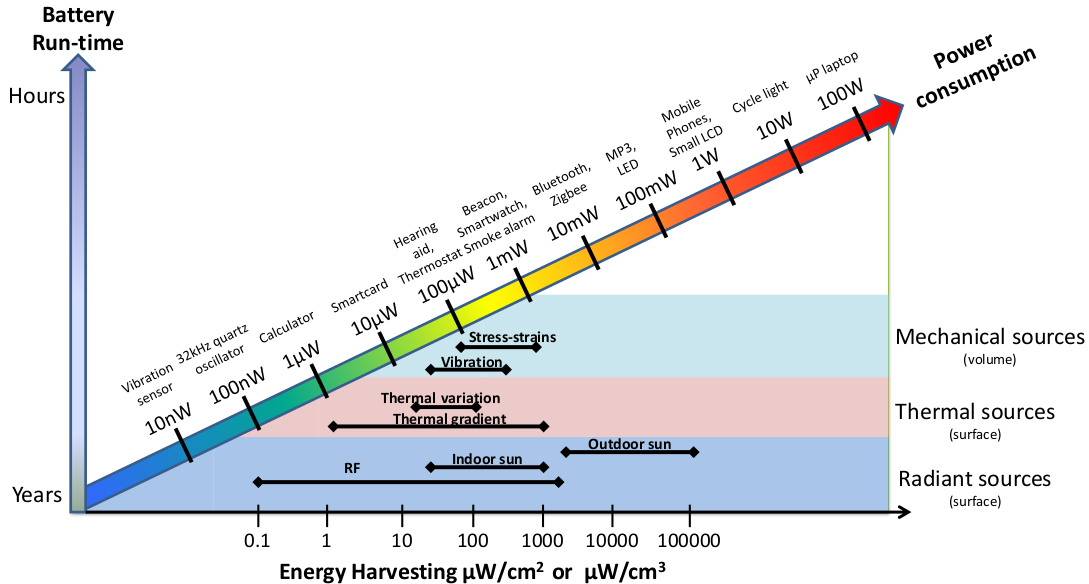
\includegraphics[width=\textwidth]{img/power_density_2.png}
   \caption{Power density of energy sources and consumption of electronic devices \cite{power_density}}
   \label{fig:power_density}
\end{figure}

Figure \ref{fig:power_density} shows power density of different energy sources and power consumption of electronic 
devices. It is seem  that the above discussed energy sources have a low power density which means very low power 
and some low power micro-electronic devices only have the privilege of integrating energy harvesting techniques 
so far. For most of the devices, the harvested power is not high enough to drive them yet. This means perpetual 
high density energy source is yet not realisiable for most of the devices. But what about wireless transfer of 
alreadry available power? We will discuss it ahead. 
%we observe the trend of technology development in reducing power consumption of micro devices and at the same 
%time, the progress in R\&D with promising results in power harvesting, we can definitely expect that harvested 
%power will meet power requirement of electronic devices in near future. But consumers' desire for battery-less 
%and wireless electronics has made the commercial electronics producers to make most use of latest advancements. 
%5This has led to integration of latest development with already matured technology for the sake of consumers' 
%satisfaction and for bigger share of the market. And hence wireless power transfer has gained much popularity. \\


\section{Wireless Power Transfer}


As discussed earlier since the evolution of battery technology is not at par with rest of the development in 
microelectronic devices and energy harvesting techniques from natural sources has not yet evolved to high power
density, wireless power transfer is by far best option to minimise challenges in battery powered devices. \\

Wireless power transfer is technique of cordlessly transferring electric energy across a air gap either to drive 
a load or to charge a battery. It eliminates the need of phycical power cables to recharge battery. and in the 
best case completely remove the battery. Wireless power transfer methods implemented today can be broadly 
classified into radiative and non-radiative power transfer on the basis of transfer distance which can be further 
sub-classified on the basis of power transfer principle \cite{wpt_fund_std} as discussed below.\\


\subsection{Non-radiative wireless power transfer}

Non radiative method of wireless power transfer based on magnetic field coupling between two coils within the distance of coil dimension. Since magnetic field diminishes rapidly after distance greater than radius of coil, assuming that distance is less than near field and far field boundary, $\lambda /2\pi$  \cite[pp. 63]{rfid_2010}, better coupling and hence power transfer can happen only within this short distance, and thus it is also called near field power transfer. Near field also means that radiative EM wave is not yet fully created and hence the name non-radiative WPT. As energy transfer in magnetic field is non radiative, it is safe even to transfer higher power as there is no RF exposure. This is one of the main reason of its widespread application today. \\

\begin{figure} [htbp]
	\begin{minipage}{\linewidth}
  	\centering 
 	 \subfloat[Inductive coupling]  {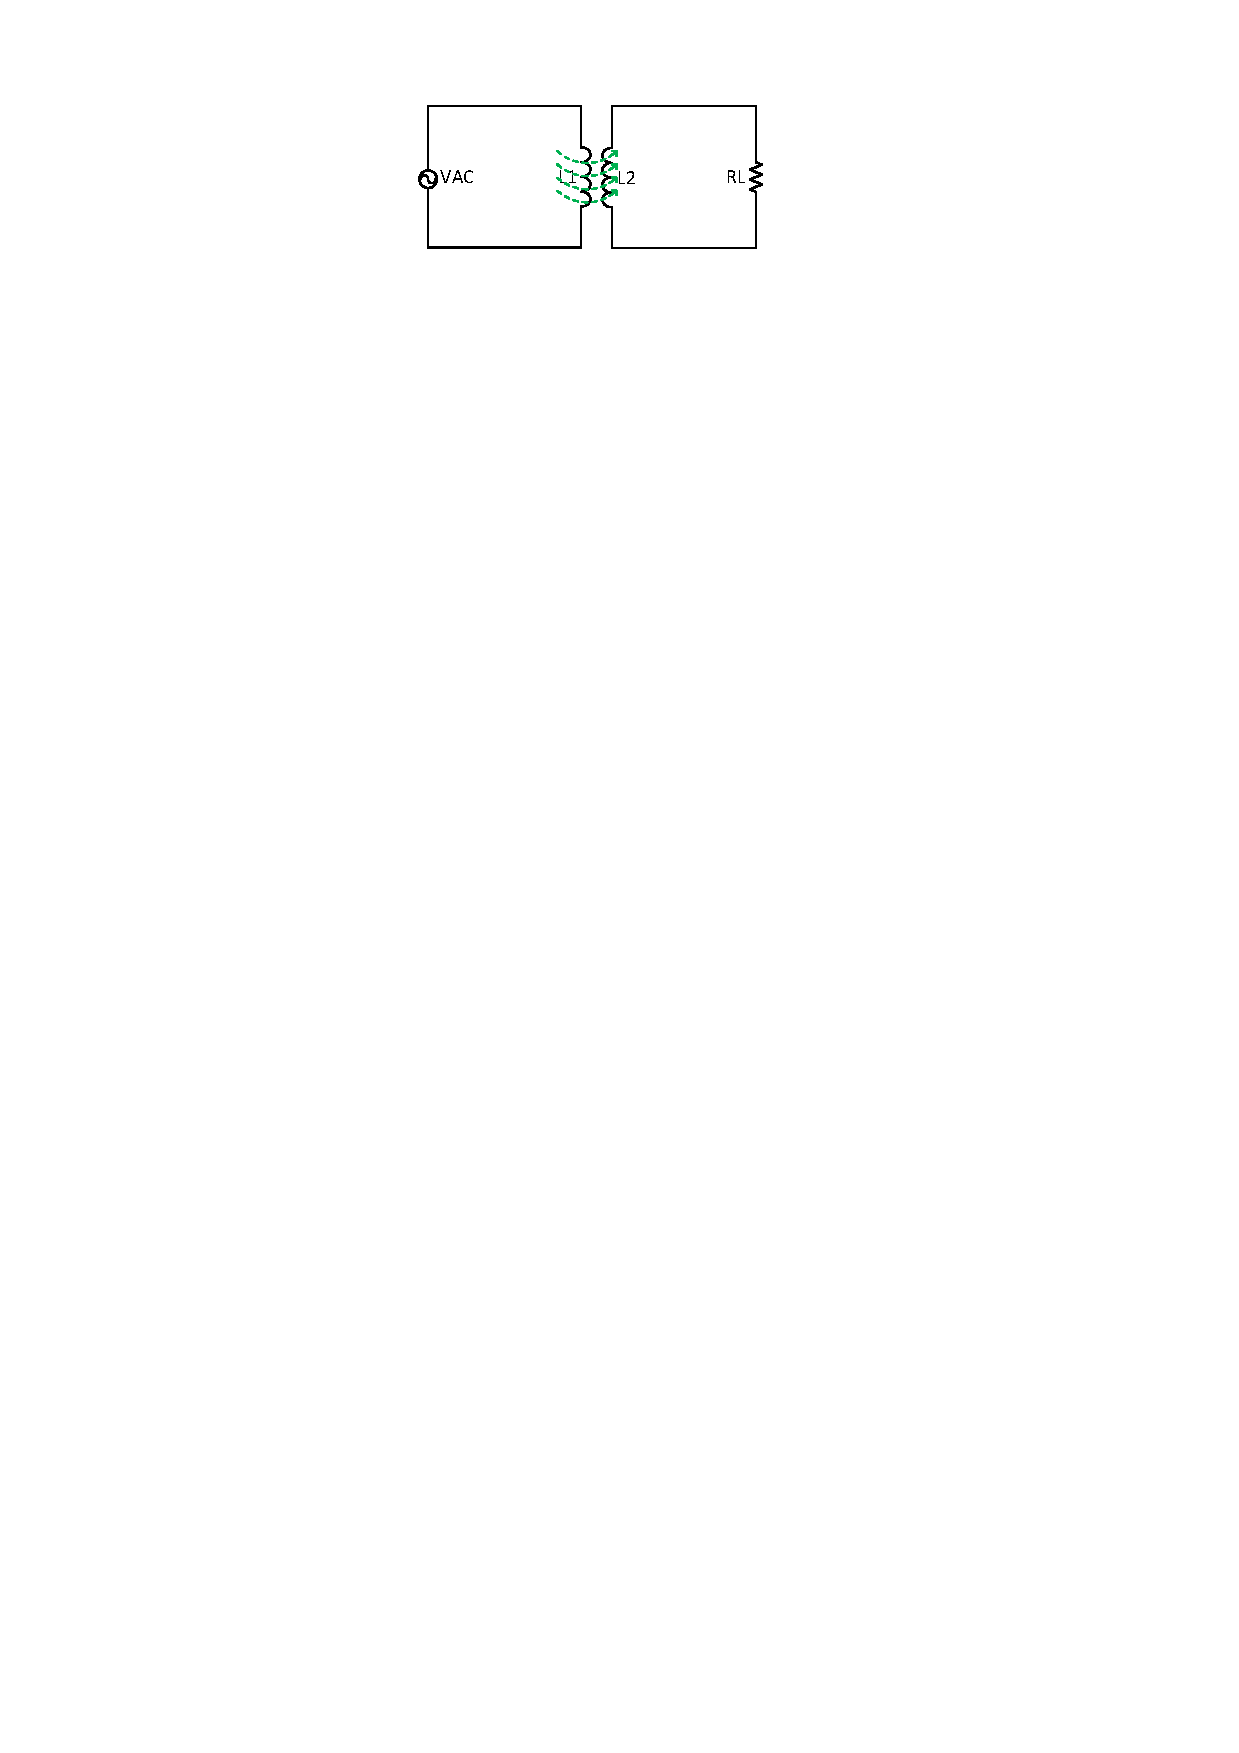
\includegraphics[width=0.48\textwidth]{img/visio_ipt.pdf} \label{visio_ipt_model}}
	 %\end{minipage}%
  	\hfill
	%\begin{minipage}{.5\linewidth}
	%\centering
 	\subfloat[Magnetic resonance inductive coupling]  {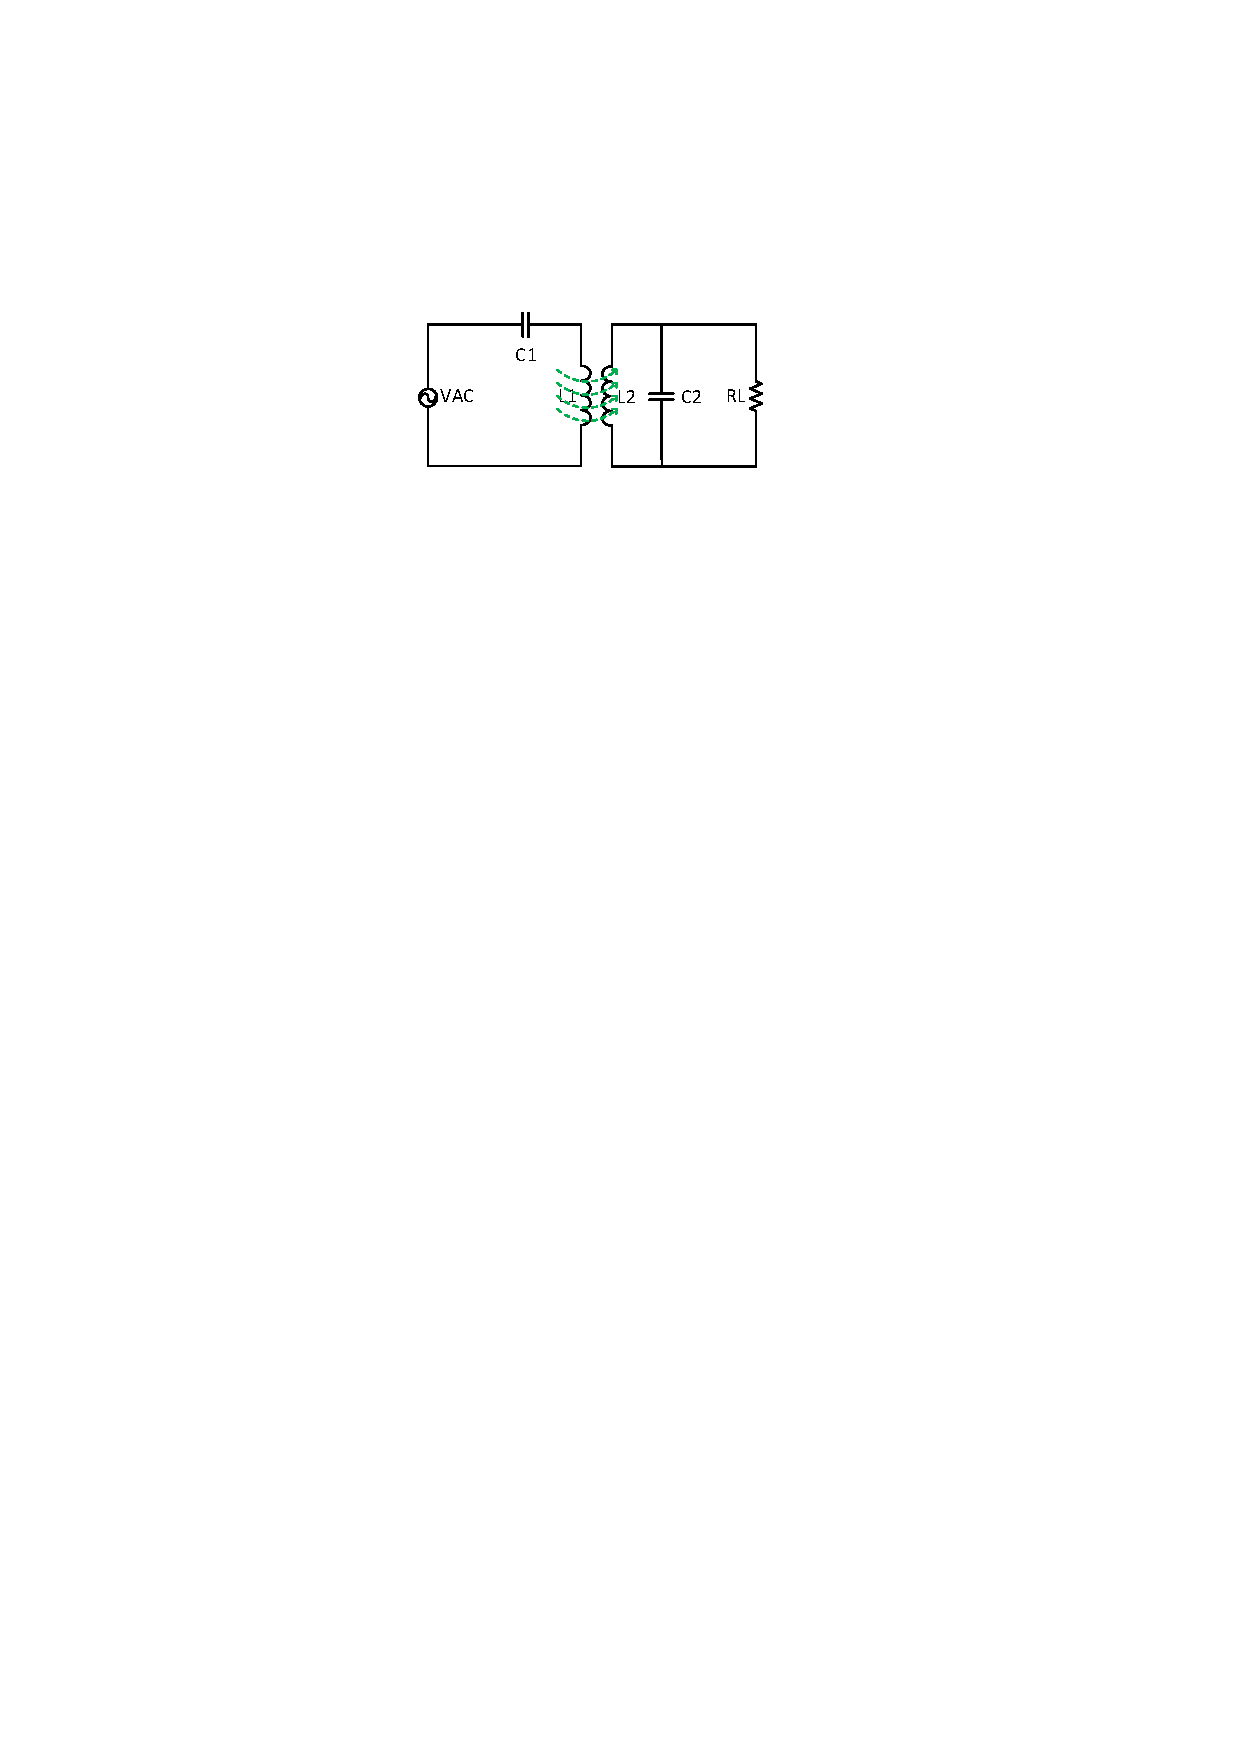
\includegraphics[width=0.48\textwidth]{img/visio_ript.pdf}\label{visio_ript_model}}
	\end{minipage}\par\medskip
 	%\hfill
	\centering
 	\subfloat[Capacitive coupling ]  {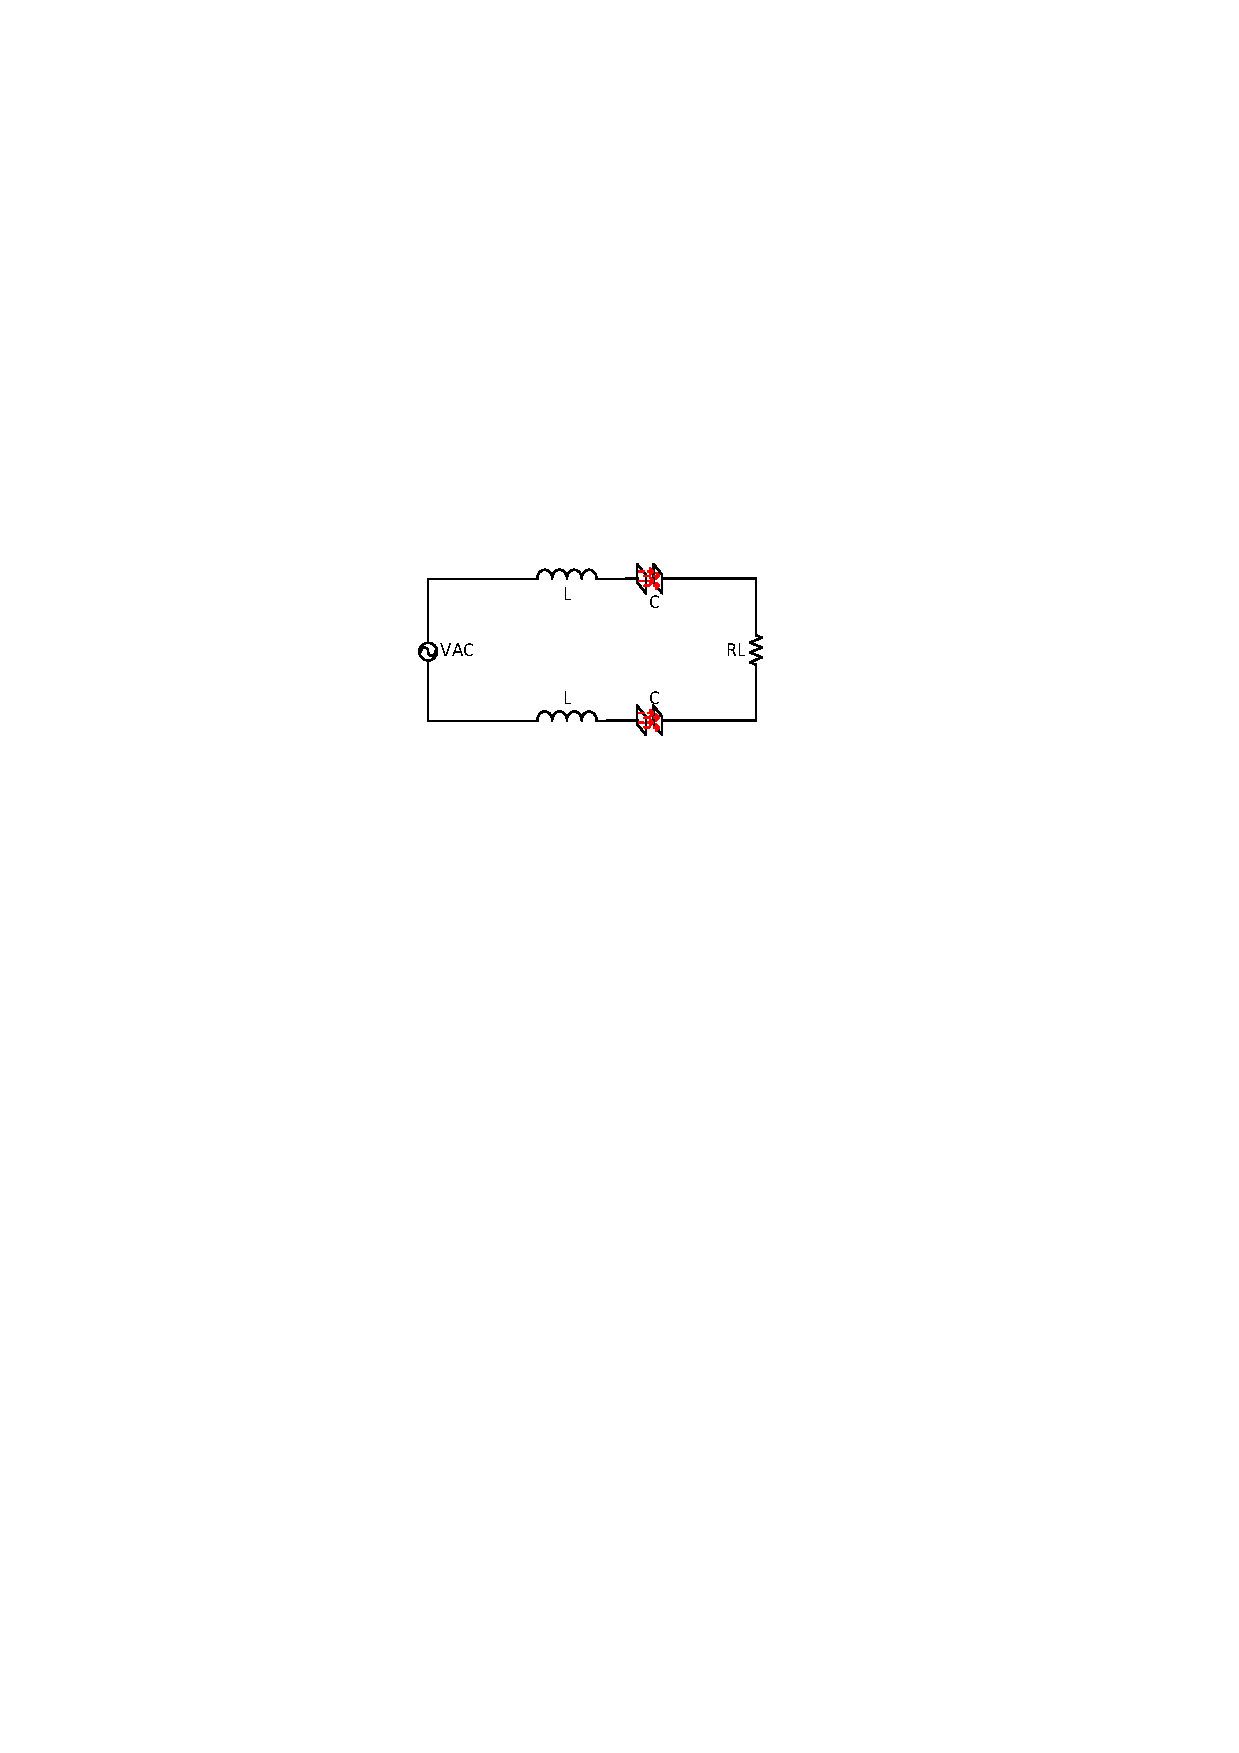
\includegraphics[width=.48\textwidth]{img/visio_cpt.pdf}\label{visio_cpt_model}}
 	\caption{Near-field coupling models} 
	\label{visio_model_near} 
\end{figure}

\subsubsection{Inductive power transfer, IPT}

IPT is based on electromagnetic induction between two coils. Electric energy is transferred by coupling of 
magnetic field from the primary to secondary coil. As stated by Faraday law of induction, alternating current 
flowing in primary coil generates varying magnetic filed which is when coupled with secondary coil includes 
voltage/current across the secondary coil. \\

In such conventional inductive coupling, larger air gap and difficulty in perfect alignment between the coils 
contribute to weak coupling, which directly translates into poor power transfer efficiency. This is why it is 
mostly used in LP devices and for short range in tens of mm transfer like RFIDs. \\

\subsubsection{Magnetic resonance power transfer}

The principle of magnetic resonance power transfer is same as IPT but with strong coupling between the coils. 
Instead of simple coil as in IPT, resonance is created at both primary and secondary coil at the same operating 
frequency. Such resonant IPT is often concisely called as  Witricity, for wireless electricity and is less 
affected by coil misalignment and physical distance compared to conventional IPT  \cite{wpt_witricity}. A very 
key application of resonant IPT is that it can be used to simultaneously transfer/charge multiple power 
receivers from a single large source coil \cite{wpt_mutliple_device_charging}. \\

Because of it strong coupling between the coils, it can effectively transfer power for mid range in tens of cm. 
It is mostly used in  wireless charging of medical implants and consumer electronics. \\

\subsubsection{Capacitive power transfer, CPT}

In capacitive power transfer, power transfer is done through capacitive coupling, use of E-field, between sending 
and receiving plates as transferring interface. For low power transfer, it is seen effective over IPT because of 
lower cost, smaller size and no shielding for EMI. However for higher power transfer is limited due to 
requirement of larger plate area and very close coupling \cite{wpt_cpt}. \\

\subsection{Radiative wireless power transfer}

Radiative power transfer used RF EM wave as a medium to deliver power. In contrary to near field, power is 
transferred through E-field of EM wave. The E-field can only develop after $\lambda /2\pi$ distance, at far 
field region, from the source \cite[pp. 112]{rfid_2010}, and energy can only be harvested in this far field 
region, it is called far field power transfer. However as EM wave is radiative and high power RF exposure has 
safety concerns on human. \\

\begin{figure}[htbp] %figure placement: here, top, bottom, or page
   \centering
   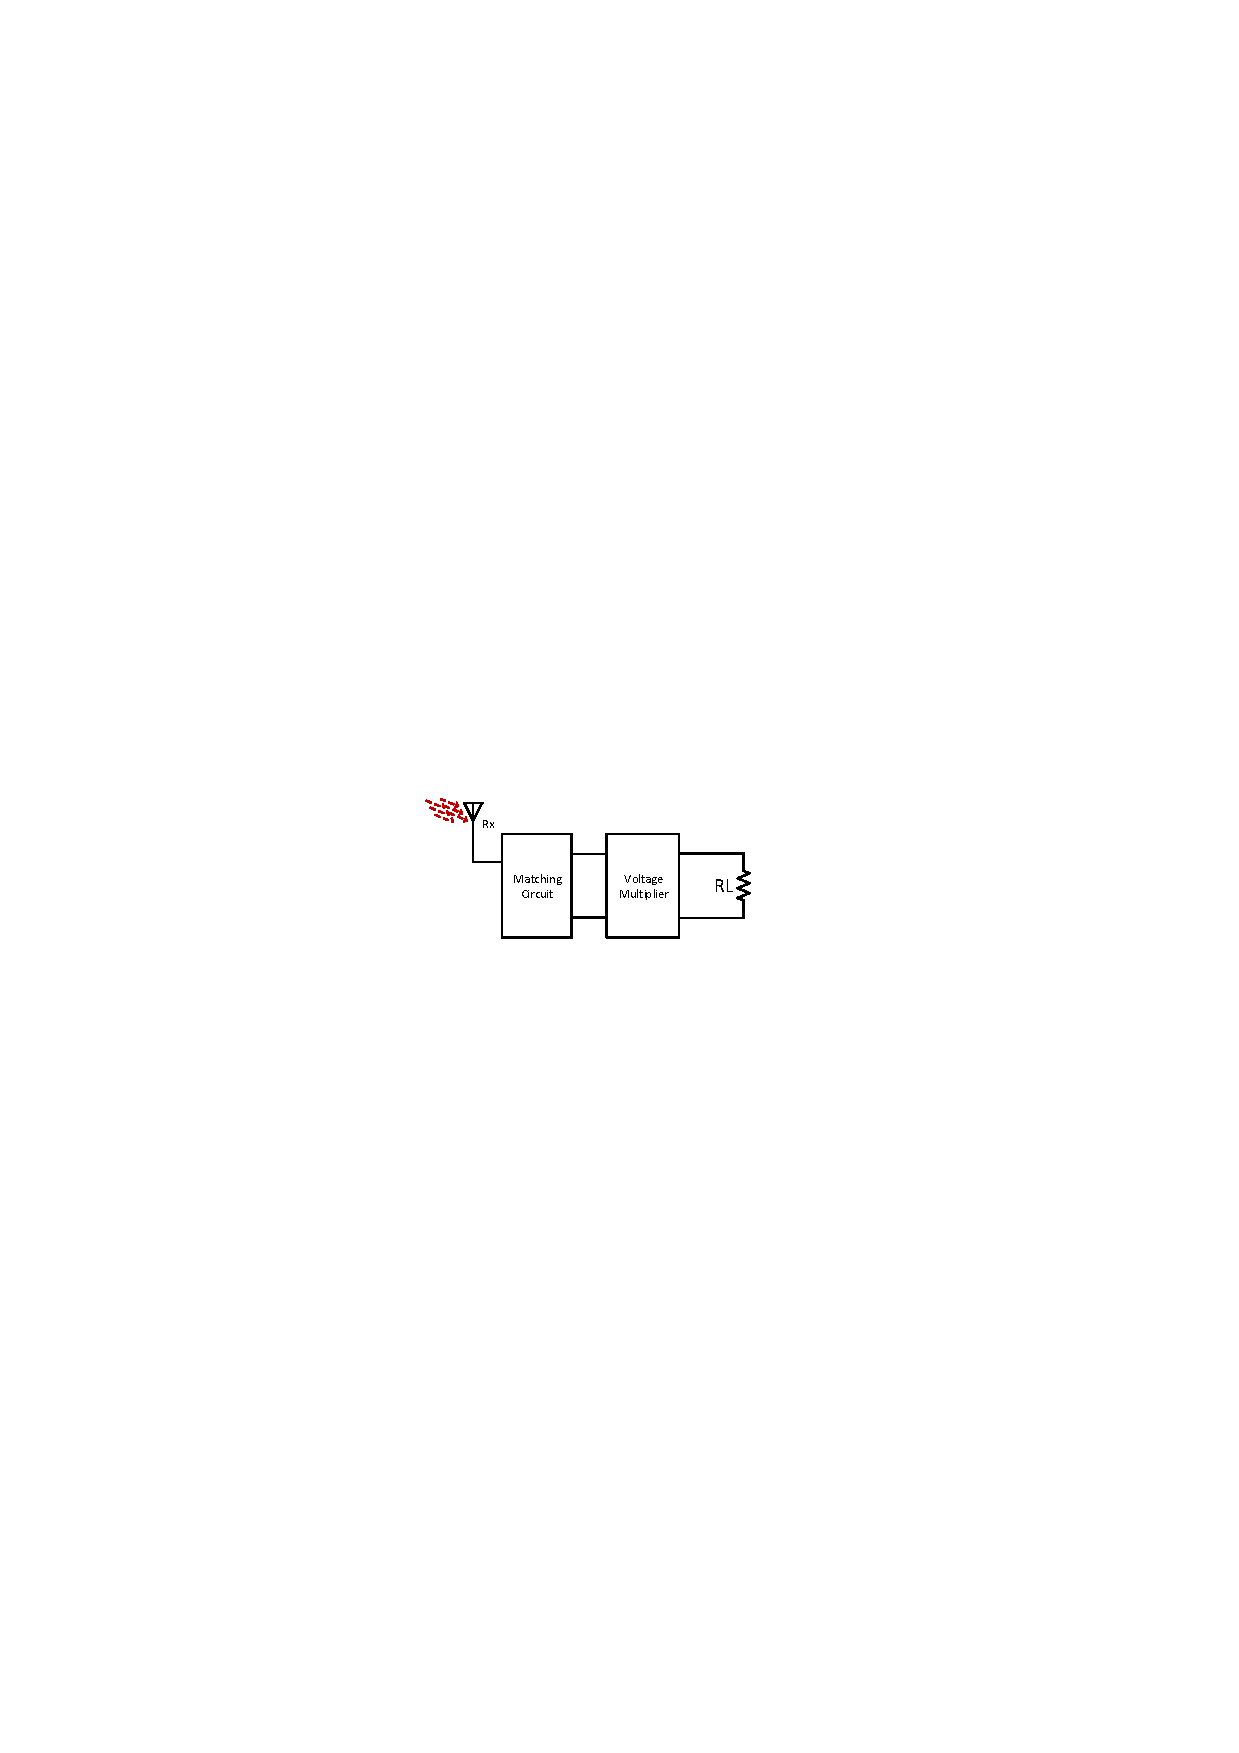
\includegraphics[width=0.65\textwidth]{img/visio_rf.pdf}
   \caption{Far-field harvesting model}
   \label{fig:visio_model_far}
\end{figure}

\subsubsection{Non-directive and directive radiative WPT}

Radiative power transfer can be divided into directive and non-directive radiative power transfer. Non-directive 
power transfer is same as discussed in EM energy harvesting, where energy is harvested from isotropically 
radiated RF wave in the surrounding.   Whereas in directive power transfer, dedicated transmitter antenna/antenna 
array is used to transmit EM wave to a particular direction of receiver antenna location. This is point to point 
far field transfer technique is also called energy beam-forming and has better transfer efficiency than 
non-directive method. \\

Health concerns as governed by \acrshort{fcc} and \acrshort{ieee} safety regulation policy on human exposure has 
limited its used to low power harvesting over longer distance using RF wave. But, as RF wave is also information 
carrier wave in wireless communication, its capacity to transmit both data and power simultaneously is expected 
to introduce new application in wireless communication field  \cite{wpt_fund_std}. \\

\subsection{WPT Applications}

It is seen today that IPT and magnetic resonance IPT are mostly used because of easier implementation, lower 
cost, wide range power transfer capability. For high power transfer in order of kilowatt, IPT is mostly used 
in the field of industrial automation like automated material handling and industrial micro-robots  and 
automotive like electric vehicle charging.  Similarly both IPT and magnetic resonance IPT are used for 
transferring power medium power up-to tens of watt. Their typical uses have been in charging battery in 
medical equipments and consumers electronics. In case of microelectronics devices like medical implants, body 
sensors, pacemaker etc, magnetic resonance IPT is mostly used both to charge a battery or directly drive the 
device. \\

\begin{figure} [htbp]
  \begin{minipage}{\linewidth}
  \centering 
  \subfloat[Qualcomm EV charger]  {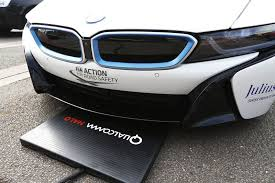
\includegraphics[width=.47\textwidth]{img/wpt_ev_qualcom.jpg} \label{wpt_ev}}
  \hfill
 \subfloat[Qualcomm mobile phone charger with foreign object detection feature]  {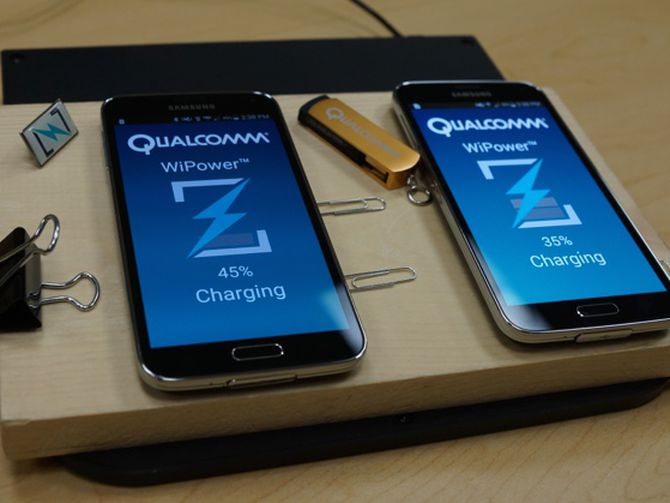
\includegraphics[width=.47\textwidth]{img/wpt_mobile_qualcom.jpg}\label{wpt_mobile}}
 \hfill
 \end{minipage}\par\medskip
 \centering
 \subfloat[IDT concept of wireless charging of bionic devices]  {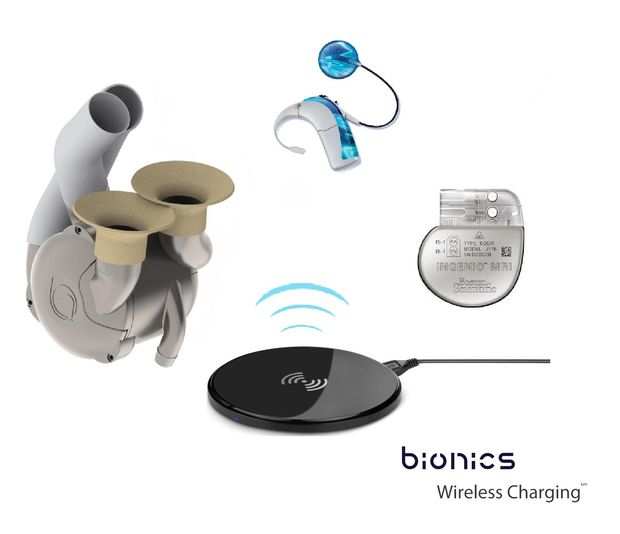
\includegraphics[width=.47\textwidth]{img/wpt_bionics.jpg}\label{wpt_medical}}
 \caption{Commercial application of wireless power transfer} 
\label{wpt_application} 
\end{figure}

In context of radiative power transfer, non-directive technique is mostly used in low power sensors and implants. 
Because of the low power requirement, mostly omnipresent RF signals are used to harvest energy. This technique 
has been used in both perpetually supplying power like in body sensor which continuously monitor some activity 
or sporadically supplying power like in RFID and body implants which work only when required. [CITE] reports 
future application of microwave power transfer can be in SPS (Solar Power Satellite) system and SHARP (Stationary 
High Altitude Relay Platform). SPS uses satellite for harvesting solar energy in space and transfer that power 
to earth. Similarly SHARP is stationary charging station for unmanned aerial vehicles in stratosphere region by 
beaming power from earth.    \\

\subsection{Charger Standards}

%http://www.radio-electronics.com/info/power-management/wireless-inductive-battery-charging/basics-tutorial.php

When wireless charging was introduced into consumer daily appliances, it was quickly realised the need of 
standard design protocols to maintain uniformity and avoid confusion for the manufacturers. Here are some 
mostly used standards in the market. All commercial standards discussed below use both IPT and resonant IPT 
techniques for charging, and have two elements: transmitter for transferring power and receiver device usually 
integrated into mobile, handheld or wearable devices. Both the transmitter and the receiver use the same control 
and management protocol in order to detect compatible electronic devices, exchange charging state information 
and control charging process. \\


\subsubsection{Qi}

\begin{wrapfigure}{R}{0.35\textwidth}
  \vspace{-5pt}
  \centering
    
\includegraphics[width=0.25\textwidth]{img/logo_qi.jpg}
  \vspace{-5pt}
  \caption{Qi}
  \vspace{-5pt}
\end{wrapfigure}

Qi standard was introduced by Wireless Power Consortium in August 2008. It has standardised two categories of 
chargers: low power charger for mobile and music players and medium power charger. The power transfer was based 
on IPT and now is operating with magnetic resonance IPT too. Qi standard allow transmitter/charger to be either 
single fixed coil, single moving coil or array of coils. The transmitter coil type determines determines the 
positioning of the receiver, either guided or free. Qi charger also have foreign object detection feature 
\cite{wpt_qi}. Qi uses the same frequency for communication and power transfer, 80-300 KHz \cite{wpt_qi_ian}. \\

\subsubsection{A4WP}

A4WP is acronym for Alliance for Alliance for Wireless Power which has introduced another independent wireless 
charging protocol. It uses magnetic resonance IPT technique for power transfer. The main differences between 
A4WP from Qi are multiple device charging from a single charger, also called power transmitting unit, PTU and 
longer charging range. Similarly there are different category of PTUs from 1 to 5, most of them still on roadmap 
and supports wireless charging from low power to high power. A4WP used different frequency band for communication 
and power transfer, which are 2.4 GHz and 6.78 MHz respectively  \cite{wpt_a4wp_ian}.\\

\subsubsection{AirFuel Alliance}

\begin{wrapfigure}{R}{0.35\textwidth}
  \vspace{-5pt}
  \centering
    
\includegraphics[width=0.25\textwidth]{img/logo_airfuel.jpg}
  \vspace{-5pt}
  \caption{AirFuel}
  \vspace{-5pt}
\end{wrapfigure}

AirFuel Alliance is newly crated wireless charging standard buy merging Alliance for Alliance for Wireless Power, 
A4WP and Power Matters Alliance, PMA in 2015 with backing of major device manufacturers  \cite{merge_a4wp_pma}. 
Like A4WP, PMA  was IPT based independent wireless charging standard. AirFuel Alliance is believed to fight the 
market dominance of Qi standard. AirFuel is expecting to expand charging standard beyond consumer electronics to 
industrial, medical and military applications \cite{airfuel}.\\

%https://www.chargespot.com/news/airfuel-and-what-it-means-for-the-wireless-charging-industry/
%https://www.airfuel.org/index.php/home/about-us-2

\section{This project}
As mentioned in the last chapter, a typical microelectronics system, BLE, used extensively in all portable and 
wearable is taken as a reference load for this project. It requires 10 mA current from a supply of 1.8 V to drive 
BLE system. The purpose of this work will be to make a wireless power transfer system for cordlessly driving BLE 
or charging BLE battery. The target specification for this work is listed in table \ref{tab:proj_spec_tar}. \\

\begin{table}[!htbp]
\caption{Target specifications}
\begin{center}
\begin{tabular}{c|c}
\hline \hline
Technology 		& TSMC 90nm 9M-1P\\ \hline
Chip area 		& TBA mm\textsuperscript{2} \\ \hline
Input AC voltage	& 2.5 Vp \\ \hline
Operating frequency  	& 13.56 MHz \\ \hline
Maximum load 		& 10 mA \\ \hline
Output DC voltage 	& 1.8 V \\ 
\hline \hline
\end{tabular}
\end{center}
\label{tab:proj_spec_tar}
\end{table}

Figure \ref{fig:funct_block} is the functional block diagram of proposed implementation of wireless power transfer in 
this work. From the discussion in wireless power transfer section, it is seen that IPT is the best option for 
being mature, easy and safe implementation. Since tuning the IPT transfer link at the operating frequency 
increases the transfer effieicency, magnetic resonance link is designed for this work. The antennas are designed 
with the specifications provided by NORDIC. The power management system includes rectifier, LDO and reference and bias circuit. The biasing and reference circuit is designed solely for 
learning the design technique without much effort on the accuracy of the generated biases and references. So 
externally supplied bias and reference will be the secondary option. \\


\begin{figure}[!htbp] %figure placement: here, top, bottom, or page
   \centering
   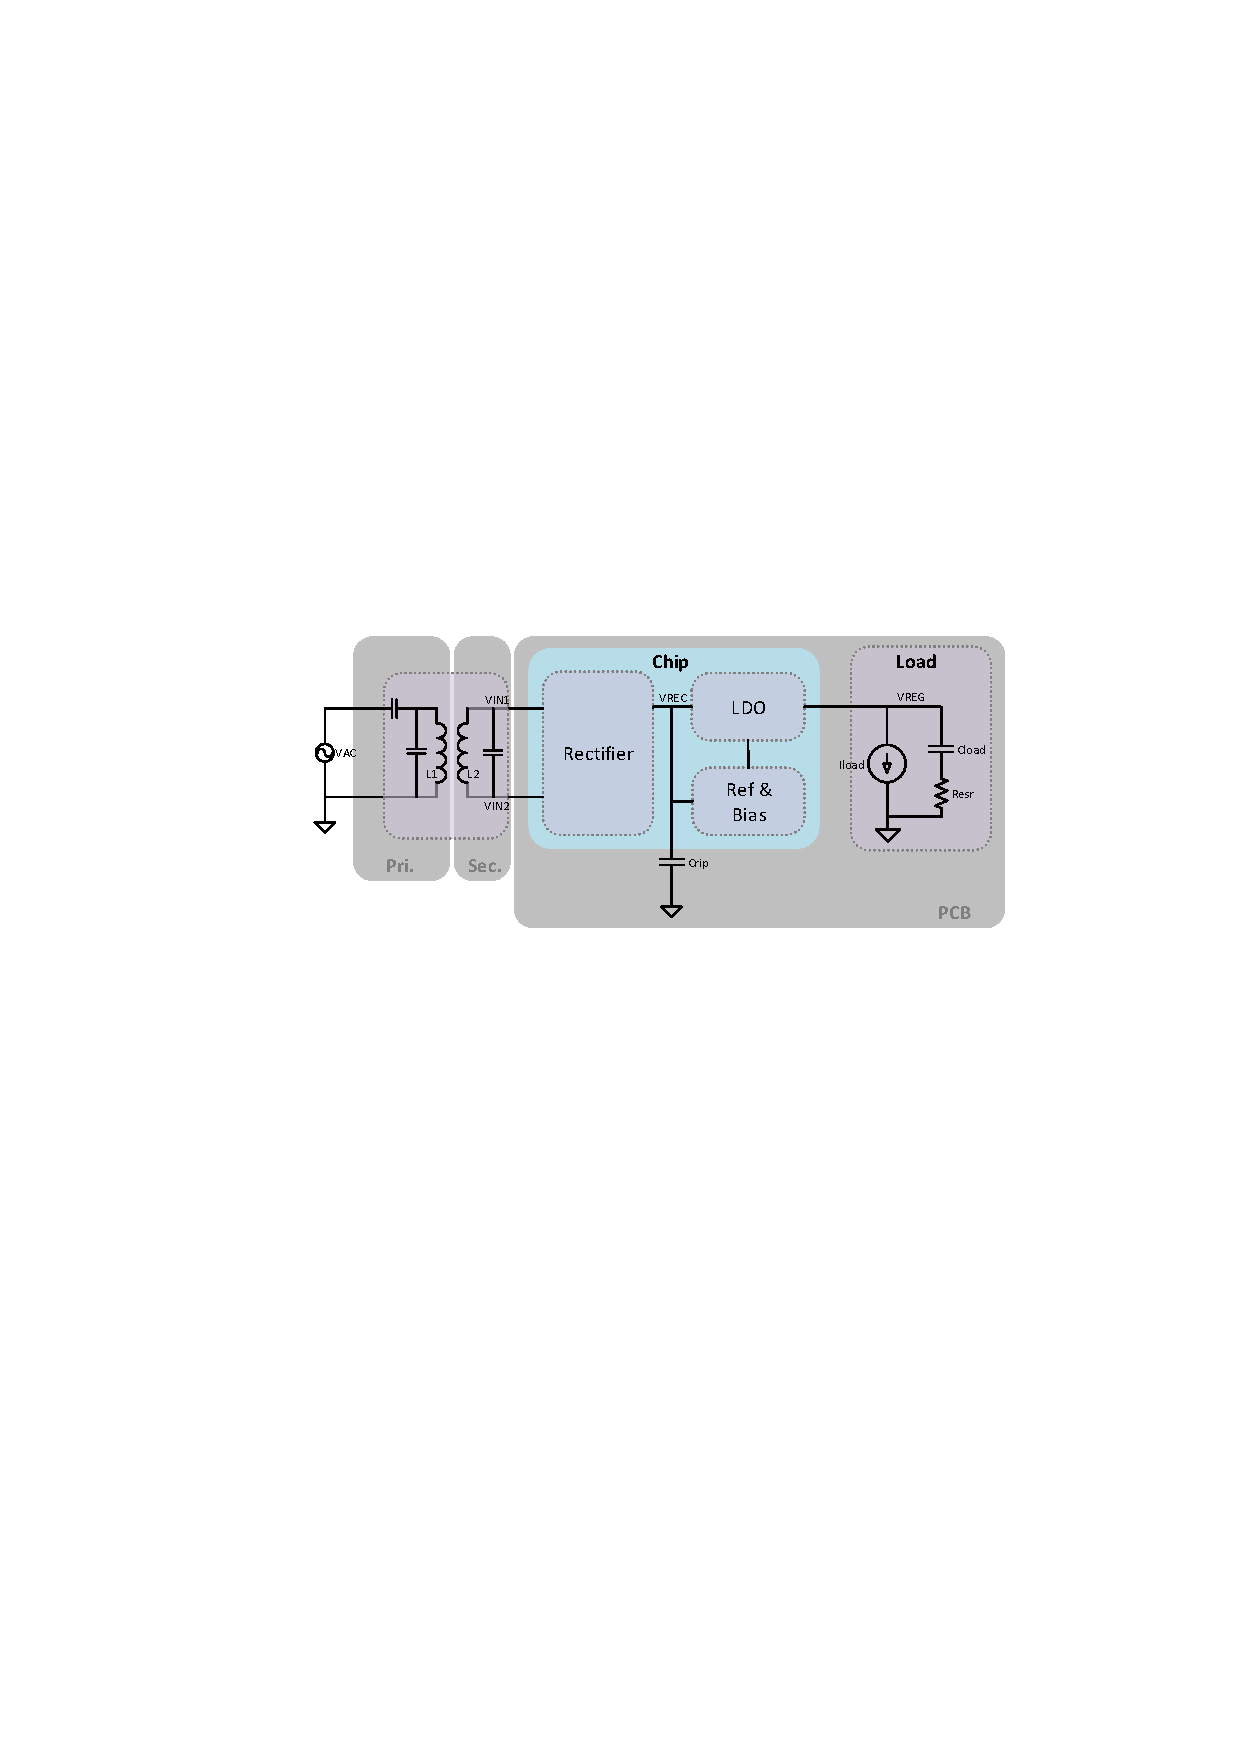
\includegraphics[width=\textwidth]{img/visio_funct_wpt.pdf}
   \caption{Functional block diagram of complete design}
   \label{fig:funct_block}
\end{figure}

The chapter ahead discusses the design, analysis and implementation of the functional blocks in figure 
\ref{fig:funct_block} starting with rectifier. The physics behiend each block is less discussed, however the 
design choices and reasoning of choices will be clearly stated. 


% *********************************************************************** RECTIFIER  ********************************************************************************************

\part{Component Design and Analysis}    

\chapter{Rectifier}  

\section{Introduction}	 	%****************************

The most basic rectifier is conventional full wave bridge structure where the diodes are replaced by the diode connected \acrshort{mos}. devices in \acrshort{cmos}. technology. This topology though being simple to implement, has a major drawback. It requires at least twice the $\acrshort{vtn}$ of a MOS device as there are two diode connected MOSes in the conduction path for each cycle of the input signal.  \\

Gate cross coupled and fully gate cross coupled topologies are improvements over conventional full wave rectifier. In gate cross coupled rectifier, two diodes of conventional rectifier is replaced by two gate cross coupled MOSes working as switches where the voltage drop for every cycle is reduced to one threshold voltage. Similarly, in the fully gate cross coupled rectifier, all diodes are replaced by switches and hence the voltage drop is further reduced to twice the conduction drop only for every cycle. Even though this topology has least voltage drop, it suffers from the problem of reverse charge leakage because when the input ac amplitude is less than the output rectified voltage and the conducting pass devices are on simultaneously, current flows backward from output to input. \\

All the above discussed topology suffer from either large voltage drop or large power loss because of which their use are limited in low power and low voltage devices. The popular techniques for higher efficiency are using gate cross coupled rectifier along with passive or active circuitry  for controlling other two pass devices. In passive rectifier, additional circuitry including bootstrap capacitor are used to reduce or eliminate threshold voltage one of which is discussed in this paper \cite{rectboot}. However, use of on-chip bootstrap capacitors limits it use where chip area and speed is of importance. On the other hand, in active rectifier, active circuitry is used control pass devices. The use of active circuitry increase both  \gls{vce} and  \gls{pce} because the pass devices are made to conduct in linear region and hence less conduction drop, and reverse current flow can be completely eliminated and hence less power loss. However active rectifier is not problem free either. The major issue is starting of the active circuit as there is no regulated supply at the start up. \\

\section{Design}	%****************************

In this project, active rectifier is chosen, primarily for better VCE and PCE and secondarily to avoid the use large on chip capacitors. \cite{rectrcc}  and \cite{rectcomp} have discussed same active rectifier topology with a slight difference in active circuitry. \cite{rectrcc} has implemented comparator with compensating the delay of comparator's output falling whereas \cite{rectcomp} has implemented comparator with compensating both the falling and the rising delay of comparator's output in expense of added circuit complexity and power consumption. \cite{rectrcc} has been used here for its simple design. \\

Figure \ref{rect_conv}, \ref{rect_cc} and \ref{rect_rcc} is the CMOS implementation of conventional full wave bridge rectifier, gate cross coupled rectifier and proposed active rectifier in \cite{rectrcc}. The problem with \ref{rect_conv} and \ref{rect_cc} has already been briefly mentioned above. Though  \ref{rect_cc}  is significantly improvement over  \ref{rect_conv} , it is still not a favourable topology with respect to the design technology chosen. In the gate cross couple rectifier of  \ref{rect_cc}, the cross coupled pMOSes act as switches, so the only voltage drop across them is conduction drop due to channel resistance. However the other two nMOSes are diode connected, so they have at least $Vtn$ drop across them which means $Vac \geq Vdc + Vtn$ for conduction. \\

\begin{figure} [htbp]
  \centering 
  \subfloat[Conventional full wave bridge rectifier]  {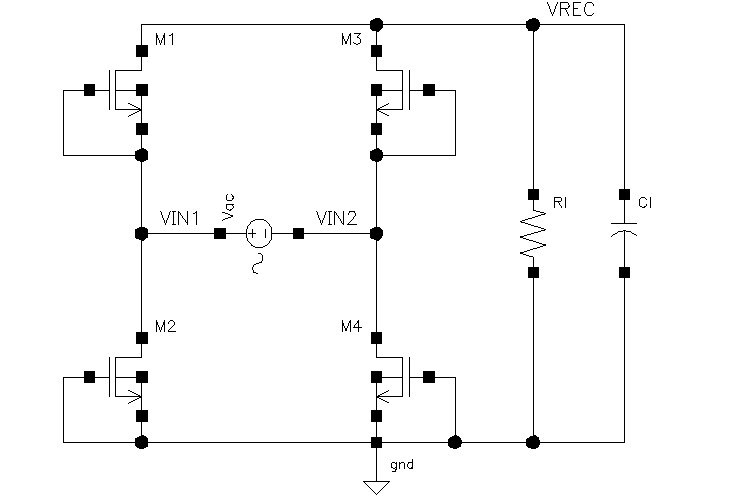
\includegraphics[width=.49\textwidth]{img/rectifier_full_bridge.pdf} \label{rect_conv}}
\hfill
 \subfloat[Gate cross coupled full wave rectifier]  {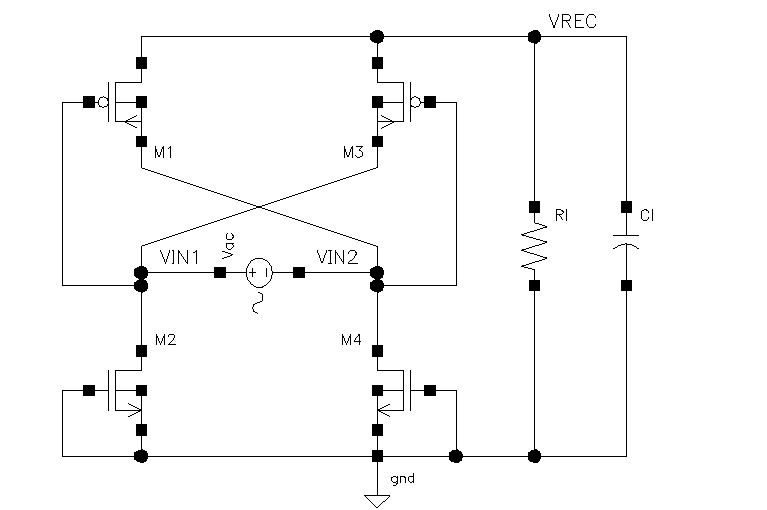
\includegraphics[width=.49\textwidth]{img/rectifier_full_cc.pdf}\label{rect_cc}}
 \caption{Rectifier topologies: conventional and gate cross coupled} 
\label{rect_conv_cc} 
\end{figure}

The proposed active circuit in \ref{rect_rcc} is improvement over \ref{rect_cc} which eliminates $Vtn$ drop required for conduction by replacing diode connected nMOS with devices controlled by active circuit as shown in figure \ref{rcc}. The active circuit is a four input comparator that turns on nMOSes fast when Vac > Vdc and turns off fast to avoid flow of current. \\

For the illustration of operation of comparator, consider the case when $Vin1 > Vin2$ i.e. $Vin1 > 0$ and $Vin2 < 0$. During this half cycle, comparator $D1$ output is low and turns off $Mn2$ and also, $Mp1$ is reversed biased and hence there is no path to flow current along $Mn2$ and $Mp1$. For simplicity, assume $Vac =  Vin1 - Vin2$. When $Vac$ reaches $\acrshort{vtp}$, $Mp3$ turns on which shorts $Vin1$ to $Vrec$. When $Vac > Vrec$, $D2$ output goes high, which turns on $Mn4$ and starts the conduction path for the first half cycle and starts charging $Cl$. When $Vac$ reaches maximum, it starts to decrease and at $Vac < Vrec$, conduction stops as output of $D2$ is low and $Mn4$ is off. As $Vac$ further decreases to below $Vtp$, $Mp3$ if off too. This way rectifier in \ref{rect_rcc}  conducts during positive half cycle eliminating the $Vtn$ drop seen in \ref{rect_cc}. Now the only drop is the conduction drop due to channel resistance of two pass devices along the conduction path. This drop is much less because during conduction both the device are operating in the linear region with small resistance. The operation is similar for $Vin2 > Vin1$ where $Mn4$ and $Mp3$ are off and $Mn2$ and $Mp1$ conduct to charge $Cl$. \\

\begin{figure}[htbp] %figure placement: here, top, bottom, or page
   \centering
   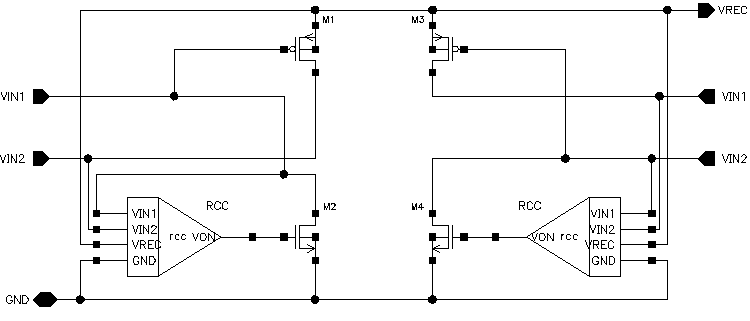
\includegraphics[width=\textwidth]{img/rectifier_schematic.pdf} 
   \caption{Gate cross coupled full wave active rectifer]}
   \label{rect_rcc}
\end{figure}

Figure \ref{rcc}  is the implementation of four input comparator $D2$ used in \ref{rect_rcc} as proposed in \cite{rectrcc}. It is designed to self power and bias because no steady state supply is available at start up. $M1$, $M2$ and $M7$ monitors voltage across $Mn4$ i.e $Vin2 - Vgnd$ and $M3$, $M4$ and $M8$ monitors voltage across $Mp3$ ie $Vin1 - Vrec$ . So when $Vin1 - Vrec > Vin2 - Vgnd$ which means $Vac > Vrec$, output of $D2$ is high and turns on $Mn4$ instantly. But when $Vac < Vrec$, the output of comparator is delayed to fall which causes $Mn4$ to conduct in reverse direction leading to significant reduction in power delivered to load. $M9$ is introduced in order to overcome this problem which adds offset currents to increase $Van$ and $Vpn$ faster, causing the output to decrease faster and turns off $Mn4$ before $Vac < Vrec$. This reverse current control technique compensates the comparator delay and increases the power efficiency of the rectifier. \\

\begin{figure}[htbp] %figure placement: here, top, bottom, or page
   \centering
   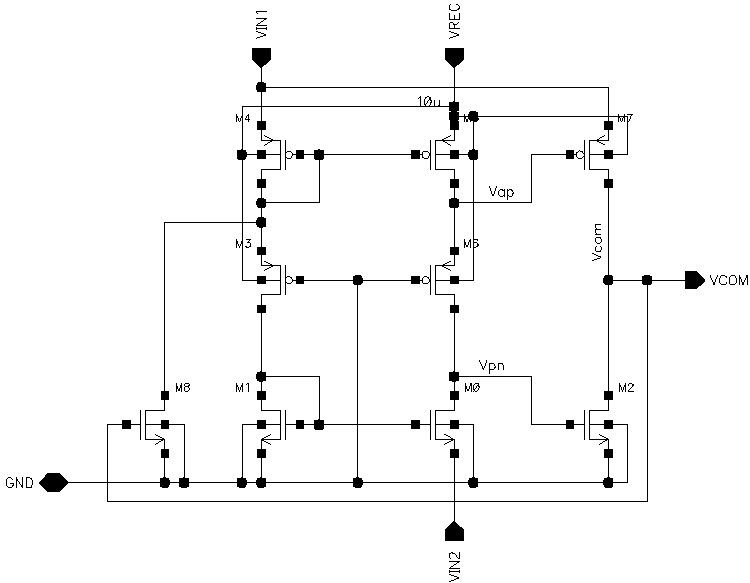
\includegraphics[width=\textwidth]{img/rectifier_rcc5.pdf} 
   \caption{Comparator circuit, RCC }
   \label{rcc}
\end{figure}

The design parameters for the rectifier is listed in table  \ref{tab:rect_parameter}. The dimensions of the pass devices are first hand calculated by using square law current equation and devices parameters values given in the technology documents, and later optimised with simulation tool in order to make the rectifier to deliver the required current. Since \acrshort{nmos} does not have to have same device size as \acrshort{pmos} to deliver same current, optimal size ratio equation from \cite{rectsize} is used to find nMOS pass devices sizes. Thought maximum load for this work is 10 mA, It is always simulated with 1 mA extra load. This extra current is to account for the fact that RCC is self powered and LDO which will follow this rectifier will be powered by $Vrec$. Similarly, the value of ripple rejection capacitor is chosen 100nF. This size of 
filter capacitor is calculated from capacitor current-voltage relationship with the assumption of keeping peak to peak ripple voltage below 5 mV to deliver 11 mA current.  \\

\begin{table}[H]
\caption{Rectifier design parameters}
\begin{center}
\begin{tabular}{c|c}
\hline \hline
Wn/Ln, Wp/Lp 		& 720um/280nm, 1.2mm/280nm \\ \hline
Rectifier area 		& TBA mm\textsuperscript{2} \\ \hline
Operating frequency 	& 13.56 MHz \\ \hline
Input ac magnitude	& 2.5  \acrshort{vp}\\ \hline
Load current 		& 11 mA \\ \hline
Ripple rejection capacitor	& 100 nF \\ 
\hline \hline
\end{tabular}
\end{center}
\label{tab:rect_parameter}
\end{table}

\section{Simulation result}		%****************************

\subsection{Transient performance}	%****************************

Figure \ref{rect_tb} is the test bench setup for simulation of the rectifier. Figure \ref{rect_plot} show the simulation results showing voltages at the input ac and output rectified DC 
voltages and current through rectifying MOSes. These  
waveforms clearly follows the working principle discussed above. Two important observations can be made from 
plots. First, the rectified output $Vrec$ is 2.2 V for $Vpp$ ac input of 2.5 V for driving which means the 
voltage loss has been significantly reduced and the loss of around 300 mV yields to the conduction loss due 
the channel resistance. Secondly, the reverse current from output to input has been effectively eliminated as 
there is only positive current flowing to the load when all conducting devices 
are on.  \\

\begin{figure}[htbp] %figure placement: here, top, bottom, or page
   \centering
   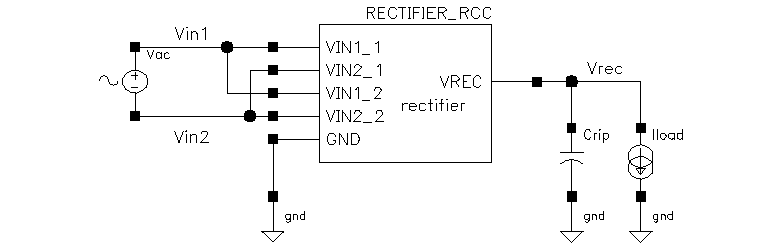
\includegraphics[width=\textwidth]{img/rectifier_testbench.pdf} 
   \caption{Testbench for rectifier}
   \label{rect_tb}
\end{figure}

\begin{figure}[H] %figure placement: here, top, bottom, or page
   \centering
   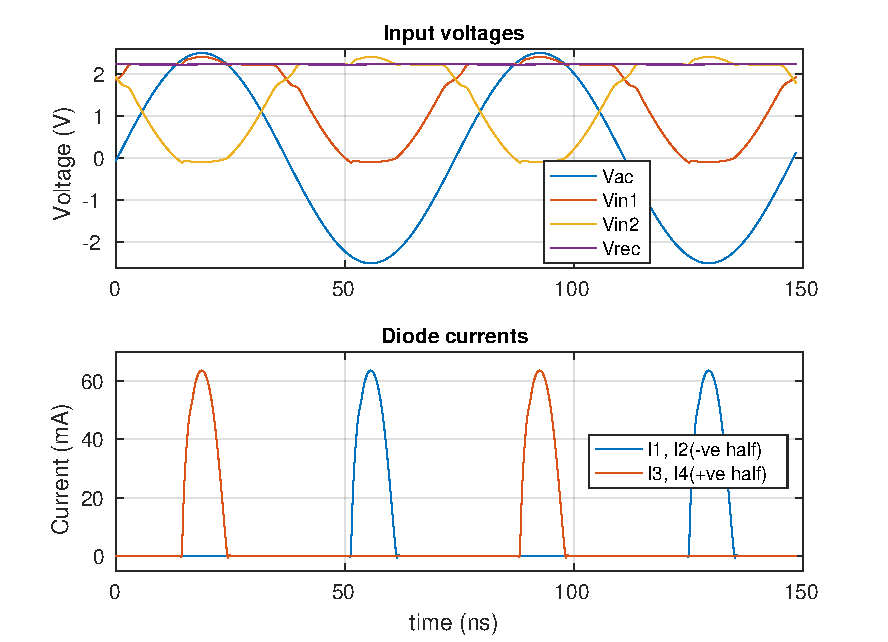
\includegraphics[width=\textwidth]{img/rectifier_VI.pdf} 
   \caption{Voltage and current waveforms of the rectifier}
   \label{rect_plot}
\end{figure}

Figure  \ref{fig:rect_v_post}  presents both pre and post layout results of input voltages, $Vin1$ and $Vin2$  and output voltage, $Vrec$, for one cycle of ac input. The closer view of rectified output is shown in figure \ref{fig:rect_ripple}. The voltage drop of about 60 mV in layout result is accounted for the voltage drop due to 
the resistance of high current conduction path. \\

\begin{figure}[H] %figure placement: here, top, bottom, or page
   \centering
   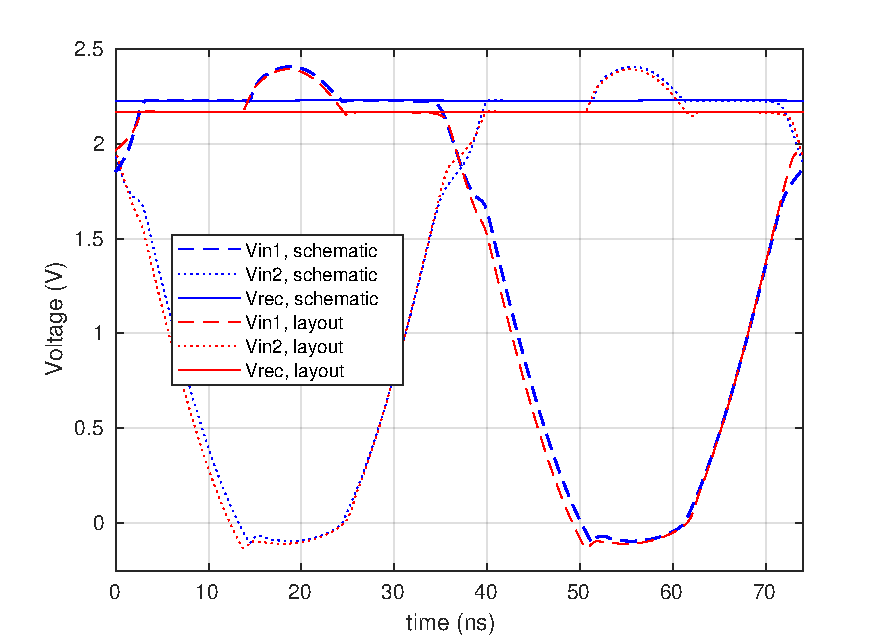
\includegraphics[width=\textwidth]{img/rectifier_V_post.pdf} 
   \caption{Voltages waveform for pre and post layout}
   \label{fig:rect_v_post}
\end{figure}

\begin{figure}[H] %figure placement: here, top, bottom, or page
   \centering
   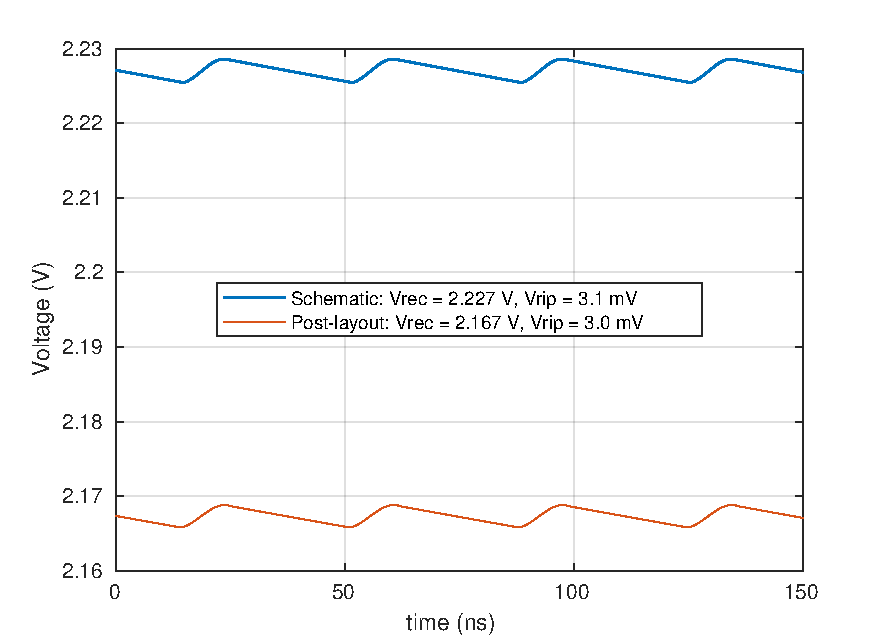
\includegraphics[width=\textwidth]{img/rectifier_ripple.pdf} 
   \caption{Rectified DC output for pre and post layout}
   \label{fig:rect_ripple}
\end{figure}

\subsection{DC performance}		%****************************

Similarly, figure  \ref{rect_ce} shows PCE, ratio of powered delivered to load to average power from the source and 
VCE, ratio of rectified DC, $Vrec$ to peak ac input, |$Vac$| with respect to magnitude peak ac input signal. |$Vac$| is gradually increased in 
peak magnitude in step of 50 mV and VCE and PCE is calculated for every step. The plot shows both 
PCE and VCE are very less for input ac amplitude less then 1.8 V. It can be explained by the fact that required 
bias current and gate drive voltage for RCC circuit are not achieved for smaller input. [INCLUDE POST LAYOUT RESULT TOO] \\

\begin{figure}[htbp] %figure placement: here, top, bottom, or page
   \centering
   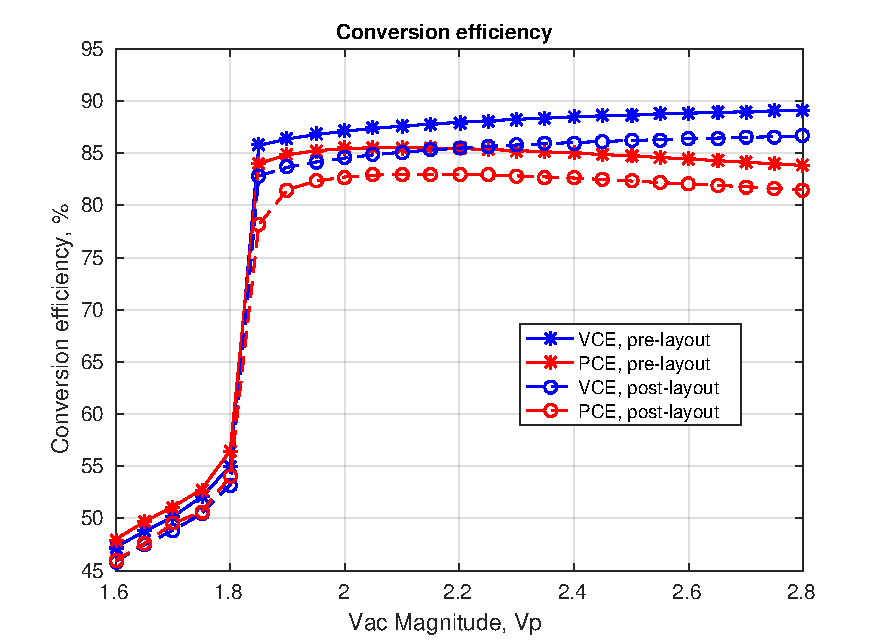
\includegraphics[width=\textwidth]{img/rectifier_ce.pdf} 
   \caption{Voltage and power conversion efficiency}
   \label{rect_ce}
\end{figure}

Table \ref{tab:rect_spec} comparatively summarises performance for pre and post layout result of the design. The layout design is attached in appendix. The layout 
is made symmetrical with four inputs, as seen in test bench figure \ref{rect_tb}, instead of two. This is done to make the current conducting path equal which result in 
equal drop in voltage when it reaches the rectifying MOSes. Simialarly the paths from the pad to the recitifier inputs are mask blocked for random metal fill to avoid 
inter layer coupling [WHY???]. The high current conduction routes are designed with wide parallel path of many higher level metal layers for reducing resistance in conduction path.

\begin{table}[H]
\caption{Rectifier performance summary}
\begin{center}
\begin{tabular}{c|c|c}
\hline \hline
				 & \textbf{Schematic}		& \textbf{Post-layout} \\
\hline \hline
Rectified DC	 	& 2.23 V 				& 2.17 V	\\ \hline
Ripple \acrshort{vpp} & 3.1 mV 				& 3 mV	\\ \hline
Peak diode current 	& 63.7 mA 			&	-	\\ \hline
PCE 				& 84.5 \% 				&	-	\\ \hline
VCE 				& 88.6 \% 				&	86.2 \%	\\
\hline \hline
\end{tabular}
\end{center}
\label{tab:rect_spec}
\end{table}

%\clearpage
%\newpage
% *********************************************************************** LDO  ********************************************************************************************

\chapter{Low Dropout Regulator}

\section{Introduction}		%****************************

Voltage regulator follows the rectifier designed above in order to regulated the rectified voltage to 1.8 V and 
deliver maximum load current of 10 mA. Since the output from the active rectifier is 2.2 V and the required 
regulated voltage is 1.8 V, charge pump or  \acrshort{smps} of boost type is irrelevant here. Buck SMPS could be 
an option for voltage regulation but LDO is preferred for it better performance in terms of noise and faster 
settling of regulated voltage.  \cite{ldo_psu}.\\ 

Figure \ref{ldo_gen} shows a circuit of typical LDO with pMOS as pass element. As shown in the figure, the 
components includes an error amplifier (EA), a pass device (Mpass), a feedback circuit (R1 and R2) and load 
(C\textsubscript{out} and I\textsubscript{load}). A more general and complete LDO circuit also includes 
circuitry for generation of reference voltage and bias current/voltage. In this project it will be discussed 
separately later. The working principle of LDO is that the error amplifier compares the scaled down regulated 
voltage, Vdiv with Vref and regulates the internal resistance of the pass transistor such that  the error, 
V\textsubscript{ref} - V\textsubscript{div} is least or zero ideally. \\

\begin{figure}[htbp] %figure placement: here, top, bottom, or page
   \centering
   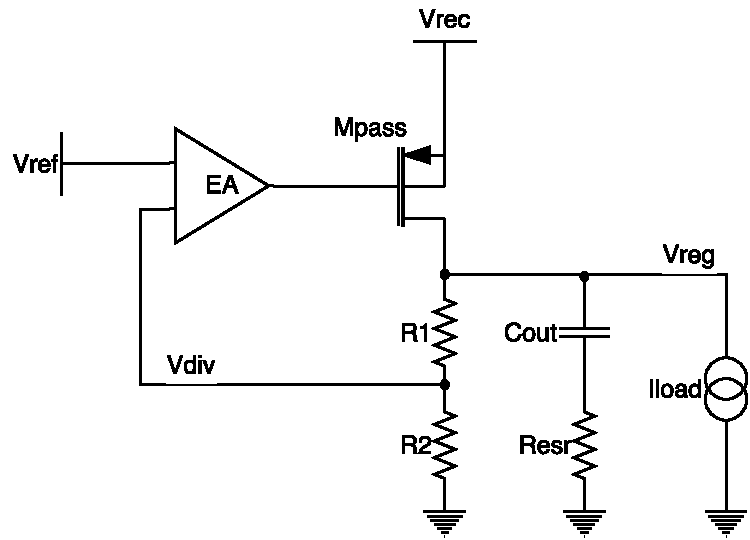
\includegraphics[width=\textwidth]{img/ldo.pdf} 
   \caption{Generic LDO with pMOS pass device}
   \label{ldo_gen}
\end{figure}

\cite{ldo_bulkmod} and \cite{ldo_quiescent} are two examples of CMOS implementation of LDO. \cite{ldo_bulkmod} 
has proposed bulk modulation technique for improving load regulation and stability of capacitor-less LDO. 
Similarly \cite{ldo_quiescent} has  proposed techniques for increasing current efficiency of LDO especially at 
no or low load condition. Though the techniques discussed in these designs have not been used, they have given 
good insight into different design parameters of LDO.  \\

\section{Design}		%****************************

Figure \ref{ldo_cmos} shows the CMOS implementation of LDO in this project. The components in this design 
include a folded cascode differential amplifier as error amplifier, pMOS buffer, pMOS pass device and feedback 
network of resistors. \\

\begin{figure}[htbp] %figure placement: here, top, bottom, or page
   \centering
   %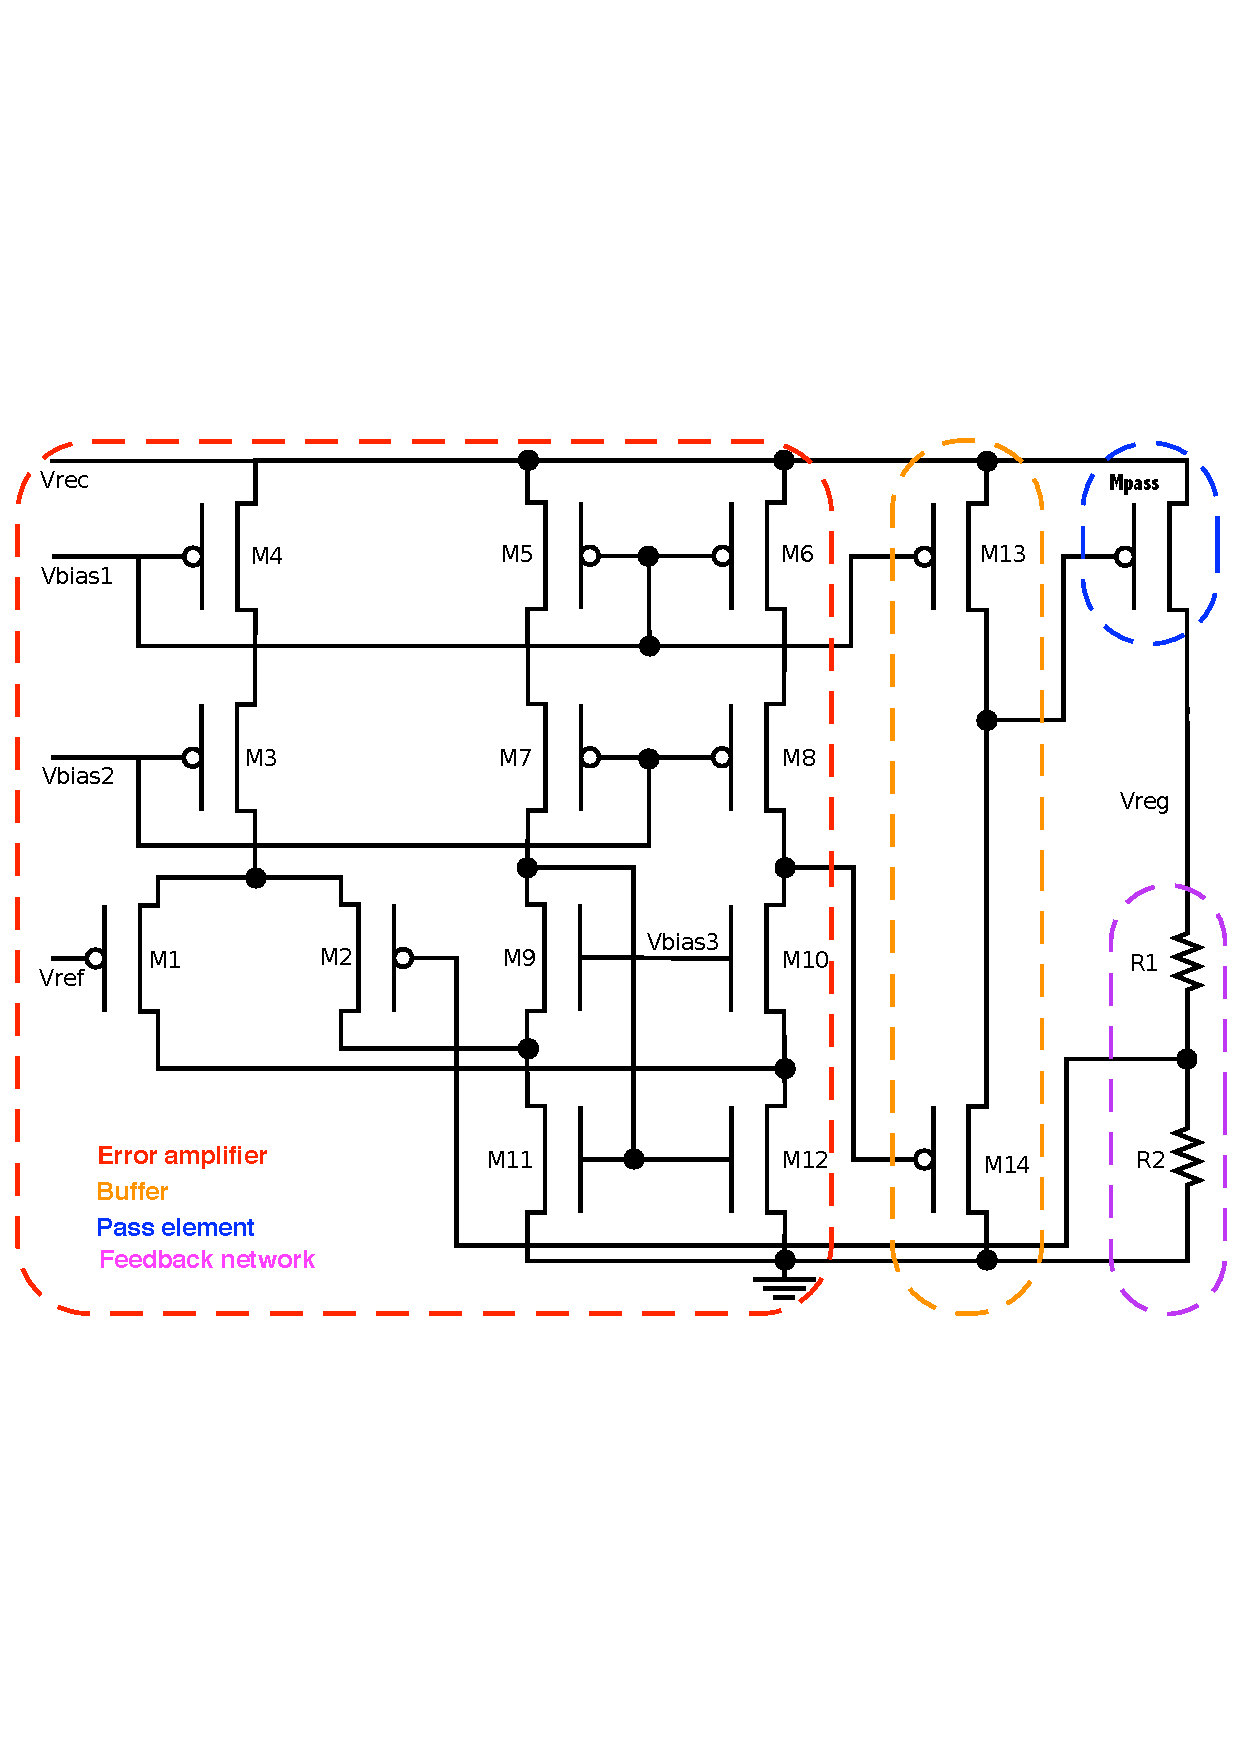
\includegraphics[width=0.9\textwidth]{img/sch_ldo_label.pdf} 
  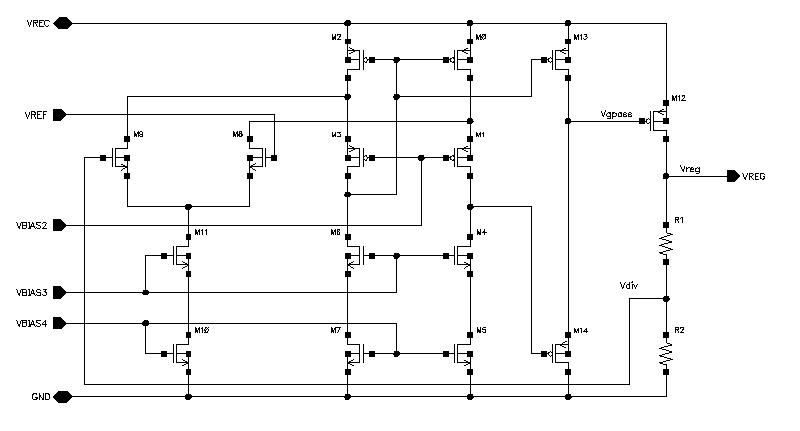
\includegraphics[width=\textwidth]{img/ldo_schematic.pdf} 
   \caption{CMOS implemenation of LDO}
   \label{ldo_cmos}
\end{figure}

As briefly mentioned above, the error amplifier amplifies the error i.e. difference in scaled regulated voltage, 
V\textsubscript{div} and reference voltage, V\textsubscript{ref}. It is known that an amplifier with higher 
open loop \acrshort{dc} gain reduces the closed loop gain error and hence amplifier with higher gain is desired 
here which is turn increase the accuracy of regulated voltage, Vreg \cite{ldo_bulkmod}. Typically error amplifier 
has gain $> 40 dB$ which is not achieved with a single stage amplifier with this technology. Higher gain can be 
achieved by cascading multiple single stage but with increased difficulty in making the multistage
amplifier stable. So for achieving higher DC gain and at the same time for stability convenience, folded cascode 
amplifier \cite[pp. xx]{razavi_2001} is chosen. \\

\begin{table}[H]
\caption{LDO design parameters}
\begin{center}
\begin{tabular}{c|c}
\hline \hline
Pass device				& pMOS \\ \hline
(Wp/Lp)\textsubscript{pass} 	& 540um/280nm \\ \hline
Input supply 				& >2.2 V \\ \hline
Error amplifier				& folded cascode \\ \hline
Vbias2 					& 1.1 V \\ \hline
Vbias3					& 0.88 V \\ \hline
Vbias4					& 0.68 V \\ \hline
Vref						& 1.17 V \\ \hline
C\textsubscript{load} 		& > 5 \si{\micro\farad}  \\ \hline
R\textsubscript{esr} 	 		& > 0.5 $\Omega$ \\ \hline
Regulated output voltage 		& 1.8 V \\ \hline
I\textsubscript{load} max. 		& 10 mA \\
\hline \hline
\end{tabular}
\end{center}
\label{tab:ldo_parameter}
\end{table}

The amplifier has a nMOS differential input stage, perferably for its higher mobility for achieving more gain.
Reference voltage, V\textsubscript{ref} will be bandgap voltage, 1.17 V, of silicon and  thus \acrshort{icmr} 
for EA lies almost at half the supply voltage. This amplifier drives a pMOS buffer which is used to supply 
sufficient current to drive the large pass transistor. Moreover, pMOS as a buffer passes 1 better which means 
it can turn off the pass device completely and hence LDO regulates better at low load or no load condition. 
However for heavier load/larger load current, this pMOS buffer is not able to pull down the gate of pass device 
suffuiciently lower. This is overcome by making the pass device large enough to feed the required  maximum 
load current.\\

The pass device is a pMOS transistor in this design. It is chosen because it has several advantages over it's 
counterparts like nMOS and BJT devices in terms of dropout voltage, quiescent current, input voltage, thermal 
response and noise\cite{ldo_ti_pmos}. Prominently, there are two factors that give pMOS edge over other devices; 
dropout voltage and quiescent current, when it comes to application in low power and low voltage devices. nMOS as 
a pass device requires a positive drive voltage with respect to output to operate. On the other hand, pMOS is 
driven by a negative signal with respect to input which means pMOS is preferable for a low input LDO. Similarly 
compared to BJTs, pMOS requires less headroom and less quiescent current to be driven\cite{ldo_ti_pmos}, 
\cite{ldo_ti_stability}, which means low dropout and low power operation, typical requirement of today's micro 
devices' power supply. \\

\begin{figure}[htbp] %figure placement: here, top, bottom, or page
   \centering
   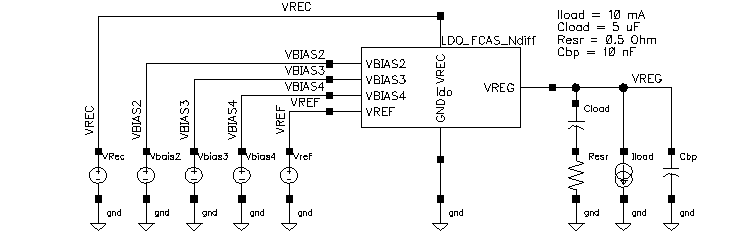
\includegraphics[width=\textwidth]{img/ldo_testbench.pdf} 
   \caption{LDO testbench setup}
   \label{fig:ldo_testbench}
\end{figure}

However, pMOS as a pass device in LDO causes challenges in stability. As mentioned above, LDO utilises a high 
gain feedback loop in order to provide a regulated output voltages independent of load current and in any system 
with feedback loop, the locations of poles and zeros determine stability of the system.  In case of the pMOS LDO, 
the pass device is configured in a common source configuration. LDO with big output cap has a dominant pole pole 
at the output, which is a low frequency pole. The second pole is located at the gate of pass device because as 
mentioned earlier pMOS pass device is large and has a big parasitic capacitance. This second pole may be located 
closer to the dominant pole, resulting in significant  reduction in phase margin (\acrshort{pm}). Consequently, 
this may lead to instability of the LDO with pMOS pass device.  Various methods have been implemented for 
ensuring the stability of the pMOS LDO. In this project, a large external capacitor, $C\textsubscript{load}$ in 
figure \ref{ldo_gen}, is used for stabilising the system at the cost of additional settling time. When an 
external capacitor is used for designing a stable LDO, the minimum value of capacitance, $C\textsubscript{load}$ 
and minumum value of its equivalent series resistance (\acrshort{esr}), $R\textsubscript{esr}$ should be 
specified\cite{ldo_ti_stability}. $C\textsubscript{load}$ determines the dominant pole of the LDO and 
$R\textsubscript{esr}$ in series with $C\textsubscript{load}$ introduces a left half plane zero below unity 
gain frequency, \acrshort{ugf} of LDO in order to cancel out the non-dominant pole below UGF, producing a 
stable LDO system. \\

\section{Simulation result}

\subsection{Transient response}	%****************************

Figure \ref{fig:ldo_tran} is the transient simulations of the LDO which illustrates generation of  regulated output voltage, $Vreg$ for 
both maximun load, 10 mA. For maximum load, it takes minimum 107 us to produce stable voltage. Since a large capacitor is used for stabilising 
LDO, it take longer time. Compared to schematic result, it takes 9 us extra time which can be accounted additional parasitic capacitance of interconnects 
at the output of LDO.\\

\begin{figure}[H] %figure placement: here, top, bottom, or page
   \centering
   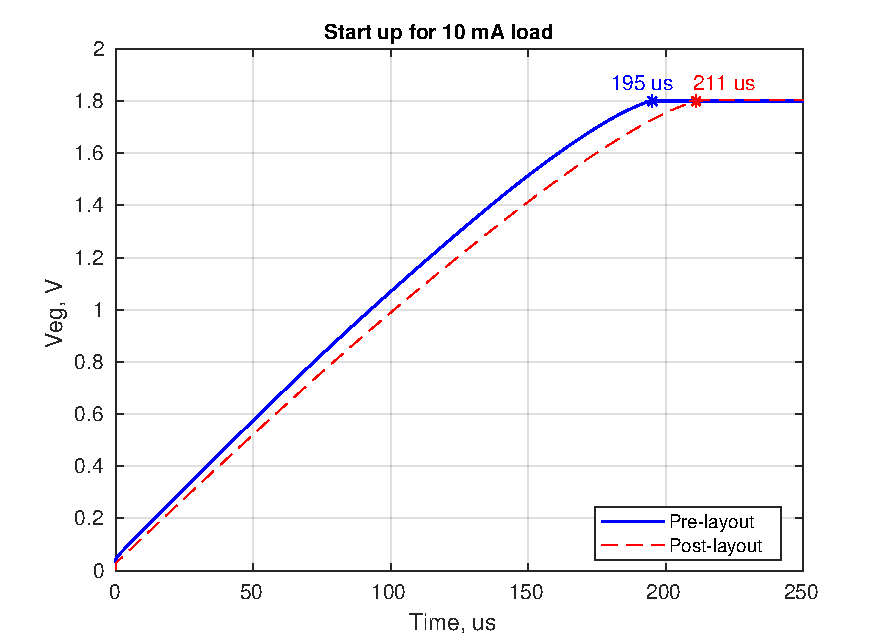
\includegraphics[width=\textwidth]{img/ldo_transient_both.pdf} 
   \caption{LDO transient simulation}
   \label{fig:ldo_tran}
\end{figure}

Figure \ref{fig:ldo_loadr} and \ref{fig:ldo_liner} show the transient response of LDO for line, $Vrec$ and load, $Iload$ variation. 
It gives information about how well and how fast regulated output settles for line and load variations. In  figure \ref{fig:ldo_loadr} load is given as pulse
 varying from 10 uA to 10 mA with both falling and rising time of 1 ns keeping input supply constant to 2.2 V. Sudden increase in load causes the output voltage to drop. The error amplifier then takes some time adjusts the gate voltage of pass device to low to fully turn on the device. Likewise when the load suddenly drops to minimum, it causes the output voltage to increase. Again error amplifier adjust it back by increasing the gate voltage of pass device to turn it off. Similarly for line variation 
 observation, input, $Vrec$ is pulsed from 2 V to 2.5 V with 1 ns rising and falling time keeping load current constant to 10 mA. Sudden increase in input voltage causes output to increase and vice-versa. As in load variation case, similar recovery pattern is seen. In both case of load and line regulation, the out put voltage is maintained 
 quickly, less than 0.15 us. Both results from schematic and post layout have same transition behaviour except post layout result offset by 3.7 mV as explained in DC response section below. \\
 
 Line regulation, change in regulated output voltage due to maximum change in input voltage and load regulation, change in output voltage due to maximum change in load current are calculated from values shown in respective plots and are listed in table \ref{ldo_spec}.

\begin{figure}[H] %figure placement: here, top, bottom, or page
   \centering
   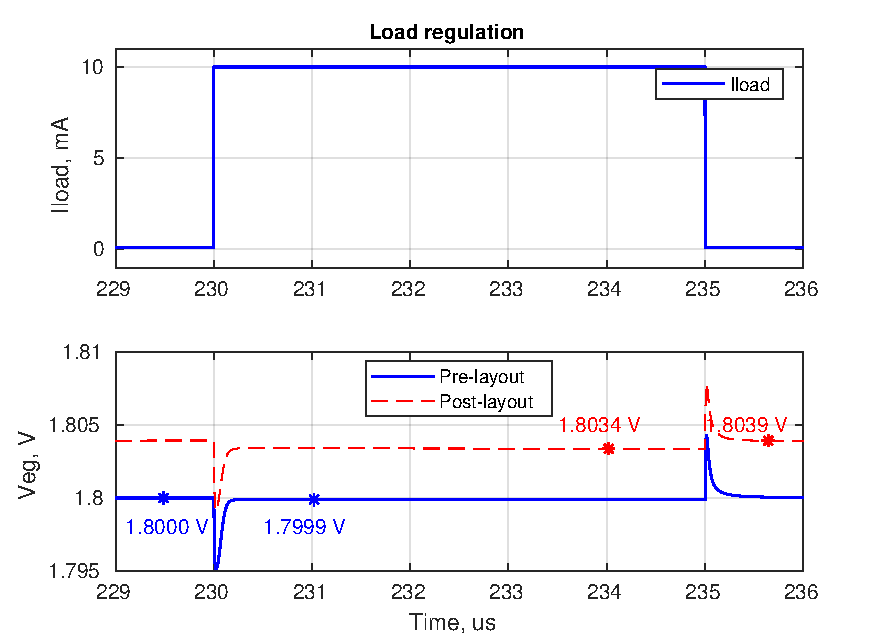
\includegraphics[width=\textwidth]{img/ldo_loadr_both.pdf} 
   \caption{LDO step load regulation}
   \label{fig:ldo_loadr}
\end{figure}

\begin{figure}[H] %figure placement: here, top, bottom, or page
   \centering
   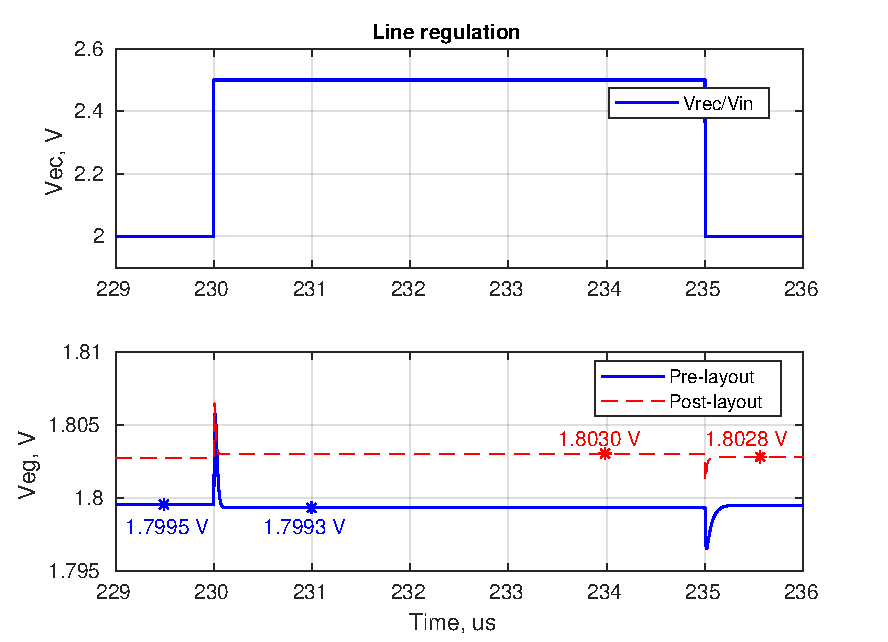
\includegraphics[width=\textwidth]{img/ldo_liner_both.pdf} 
   \caption{LDO step line regulation}
   \label{fig:ldo_liner}
\end{figure}

\subsection{DC response}		%****************************

Figure \ref{fig:ldo_dc} and \ref{fig:ldo_Iload} show LDO response to input voltage, $Vrec$ sweep and output load, $Iload$ sweep. As seen in \ref{fig:ldo_dc}, the
regulator is turned off for input below 1.85 V. Since the input is also the supply for the entire design, higher voltage is required for creating proper biasing 
of internal folded cascode error amplifier. However after turning on, it requires only 100 mV drop for proper regulation for maximum load and is even lesser for lighter 
load. This shows that minimum value of supply required for LDO to function properly is 1.95 V. In \ref{fig:ldo_Iload}, it is seen that regulated output voltage for post 
layout simulation is 3.7 mV higher than for schematic. Since $Vreg = (1 + R1/R2)*Vref$, the mismatch in the resistors has resulted in slightly higher ratio, consequently 
increasing the close loop gain.\\



\begin{figure}[H] %figure placement: here, top, bottom, or page
   \centering
   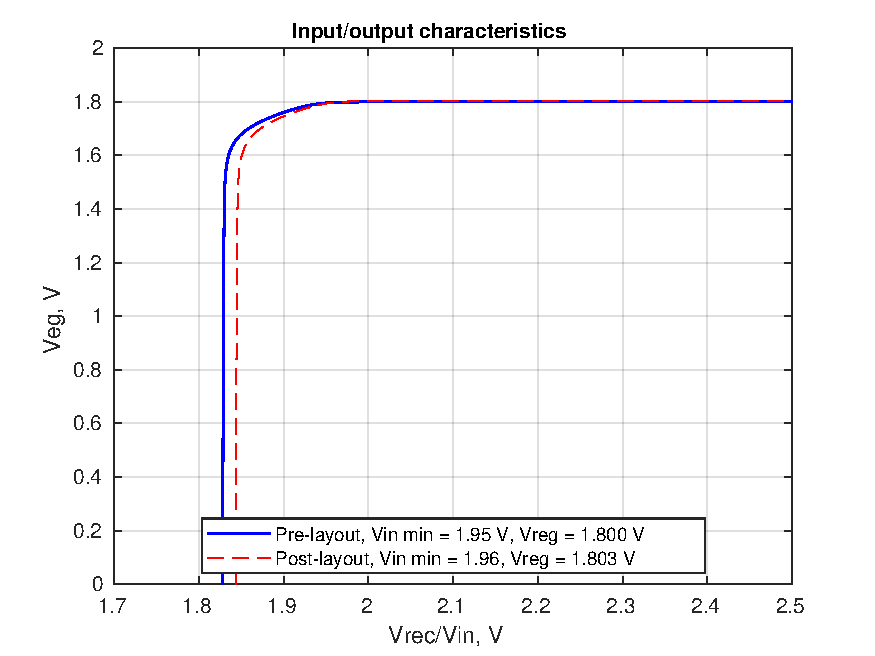
\includegraphics[width=\textwidth]{img/ldo_dc_both.pdf} 
   \caption{Regulated voltage with supply variation}
   \label{fig:ldo_dc}
\end{figure}

\begin{figure}[H] %figure placement: here, top, bottom, or page
   \centering
   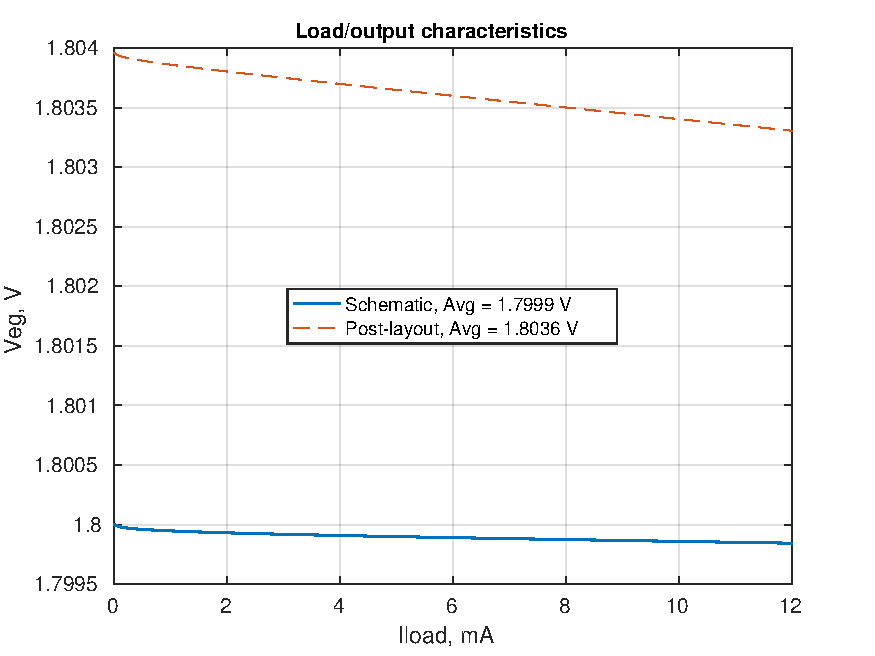
\includegraphics[width=\textwidth]{img/ldo_Iload_both.pdf} 
   \caption{Regulated voltage with load variation}
   \label{fig:ldo_Iload}
\end{figure}

\subsection{AC response}		%****************************

Figure  \ref{fig:ldo_sta} is open loop gain and phase margin of LDO without and with compensation. In the upper  uncompensated bode plot, two poles below UGF are seen: 
the first one at 300 KHz due to output resistance of pass device and its parasitic capacitance, and the second one at  60 MHz due to buffer output resistance and gate 
capacitance of pass device. UGF is at 100 MHz. Due to these two poles both occurring below UGF, the PM fallen to -45\textdegree. For making the LDO stable, as discussed  in the beginning, a capacitor, $C\textsubscript{load}$, 2.5 uF with specific series equivalent resistance, $R\textsubscript{esr}$, 0.8  $\Omega$ is used at the output.  $C\textsubscript{load}$ and pass device output resistance creates the dominant pole at 1 KHz and $R\textsubscript{esr}$ and $C\textsubscript{load}$ creates a left half plane zero below UGF which cancels the non dominant pole.  This eventually gives 75\textdegree PM and 30 dB \acrshort{gm}. \\ 

Likewise figure \ref{fig:ldo_pssr} is the plot showing \acrshort{pssr}  of this LDO. It can be seen that it has poor PSSR performance for frequency higher than 200 KHz. Low frequency noise like 50Hz supply ripple is effectively rejected. In this design 13.56 MHz ripple and its first harmonics is expected in the input of LDO because rectified 
output from rectifier operating at 13.56 MHz as input signal is used as supply and/or input for this LDO. Unfortunately, PSSR performance is worst around this 
frequencies. However the ripple rejection is still -36 dB at 13.56 MHz which is decent. As seen in figure \ref{fig:ldo_sta}, the open loop gain of LDO feedback circuit is 
90 dB, which has contributed in achieving decent PSSR even at higher frequency\cite{ldo_ti_pssr}. This paper also discusses that UGF frequency corresponds to the roll 
off frequency of PSSR, which can also been seen by comparing plots  \ref{fig:ldo_sta} and \ref{fig:ldo_pssr}. The stability technique in this design also gives adverse effect on PSSR performance as UGF is significantly lowered by large output capacitor. 
\\ 
 
\begin{figure}[H] %figure placement: here, top, bottom, or page
   \centering
   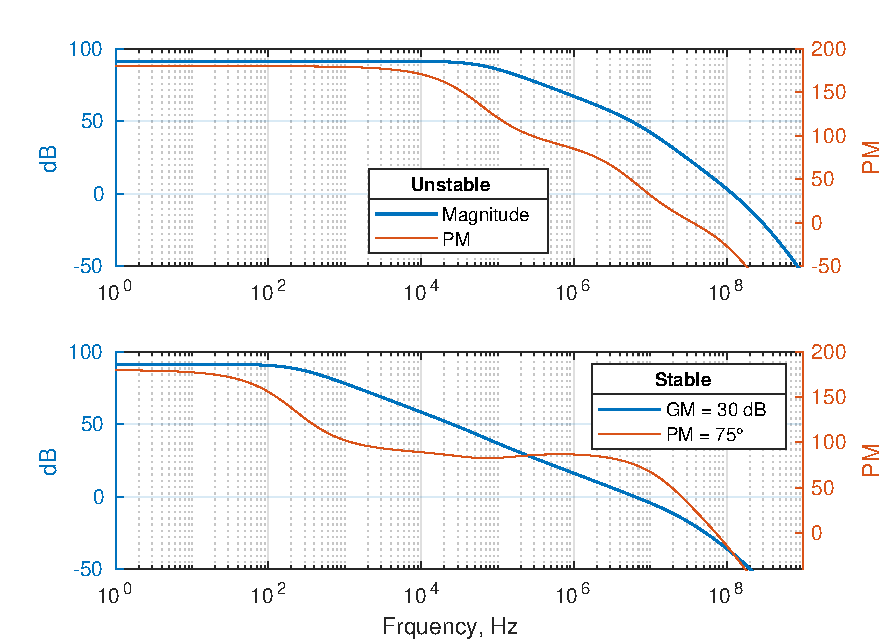
\includegraphics[width=\textwidth]{img/ldo_ac.pdf} 
   \caption{LDO stability before and after compensation}
   \label{fig:ldo_sta}
\end{figure}

\begin{figure}[H] %figure placement: here, top, bottom, or page
   \centering
   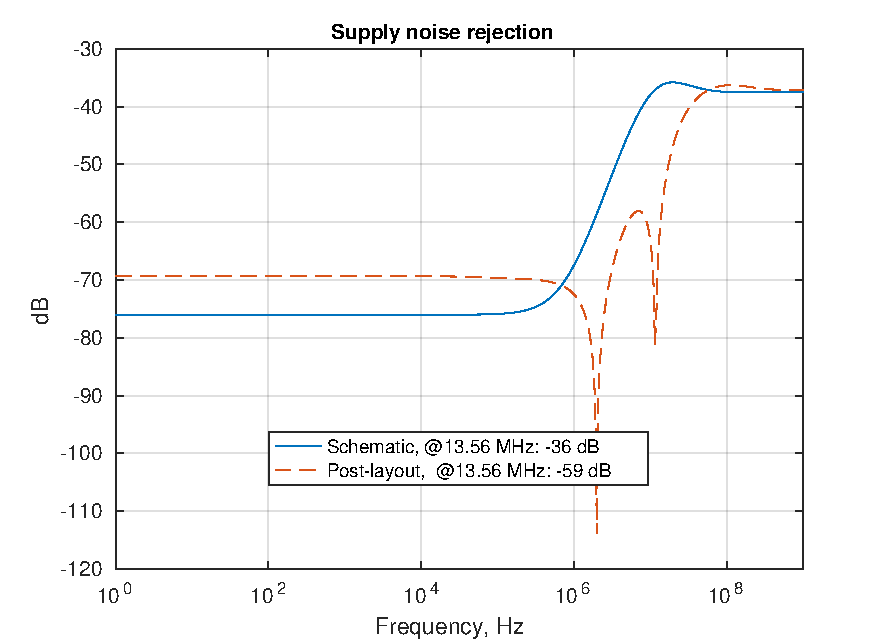
\includegraphics[width=\textwidth]{img/ldo_pssr_both.pdf} 
   \caption{PSSR performance}
   \label{fig:ldo_pssr}
\end{figure}

Table \ref{ldo_spec} summaries the performance of LDO regulator discussed above. Power efficiency is calculated as power delivered to load to power consumed 
from the source. Quiescent current includes biasing currents for error amplifier, feedback resistors and buffer which is obtained by taking the difference of current 
drawn from the source and current delivered to the load. Both power efficiency and quiescent current is calculated for maximum load operation. 

\begin{table}[H]
\caption{LDO performance summary} 
\begin{center}
\begin{tabular}{c|c|c}
\hline \hline
				 & \textbf{Schematic}		& \textbf{Post-layout} \\
\hline \hline
PSSR 			 & -36 dB	@ 13.56 MHz	&-59 dB	@ 13.56 MH\\ \hline
Phase margin		 & 75\textdegree 		&	 \\ \hline
Gain margin		 & 30 dB				&	 \\ \hline
Power efficiency		& 80.9 \%			& 81 \%	\\ \hline
Quiescent current	& 105 uA			& 114 uA	\\ \hline
Load regulation 	& 17 uV/mA			& 53 uV/mA	\\ \hline
Line regulation 		&  435 uV/V 		& -1.162 mV/V	\\ 
\hline \hline
\end{tabular}
\end{center}
\label{ldo_spec}
\end{table}%

%Reference and biasing circuit design follows next. \\


\clearpage
\newpage
% *********************************************************************** REFERENCE AND BIASING  *******************************************************************************



% *********************************************************************** ANTENNA DESIGN  *****************************************************************************************

\chapter{Antenna Design}  

\section{Introduction}		%****************************

All the components discussed above are part of any power management system which takes DC input from power line 
and creates regulated output as required. However, the objective here is to replace direct power line connection with 
wireless link. Since the intention is to just create a wireless power transfer link, the option which is easier to implement, 
convenient to operate and gives higher transfer efficiency is the primary choice here. And the literatures in wireless power 
transfer studies show inductive coupling meets all these requirement. \\

\begin{figure} [!htbp]
  \centering 
  \subfloat[Inductive coupling between two coils]  {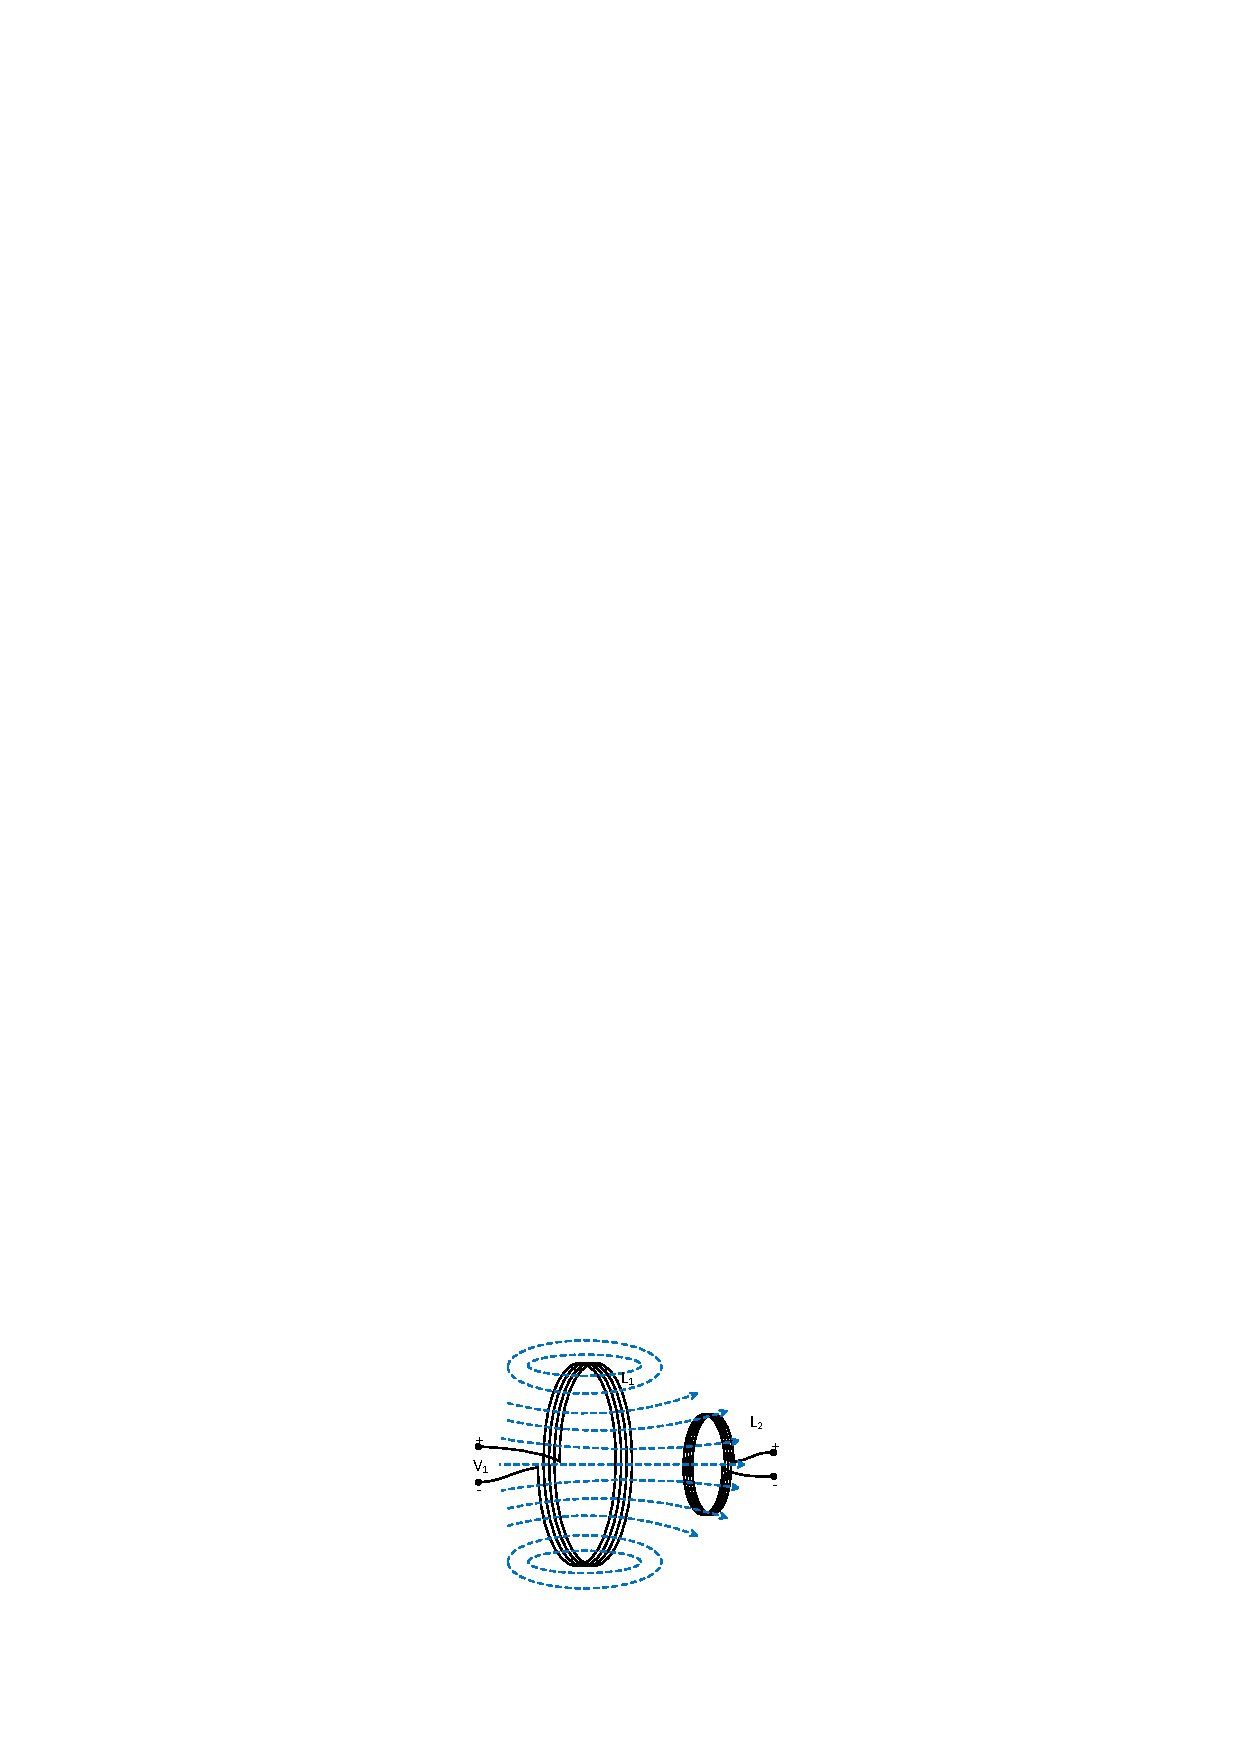
\includegraphics[width=.49\textwidth]{img/ant_induction.pdf} \label{fig:ant_induction1}}
\hfill
 \subfloat[Model of inductive coupling]  {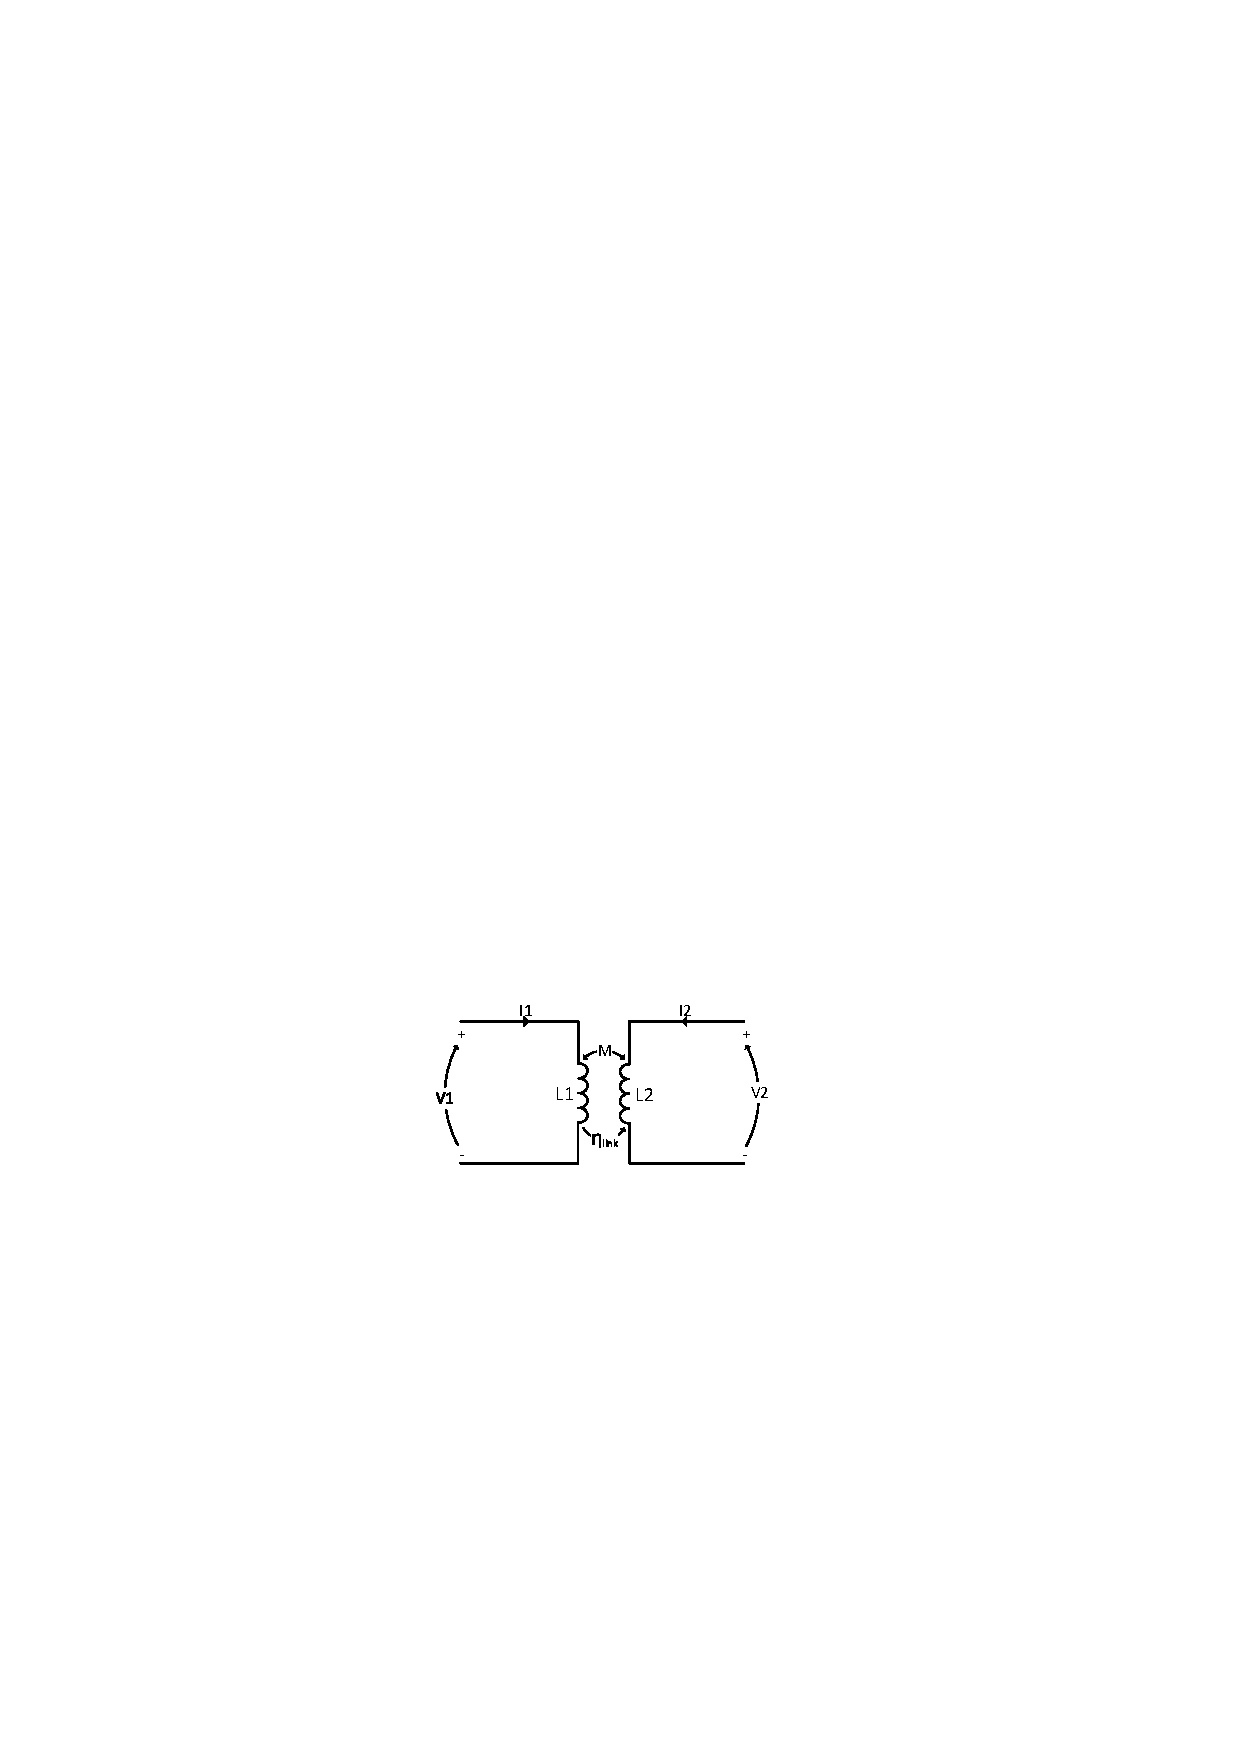
\includegraphics[width=.49\textwidth]{img/ant_induction_model.pdf}\label{fig:ant_induction2}}
 \caption{Inductive coupling } 
\label{fig:ant_induction} 
\end{figure}

Inductive coupling boils down to principle of electromagnetic induction as first discovered by Faraday, shown in figure \ref{fig:ant_induction} . When alternating electric current, $I_{1}$ is passed through 
a coil, say primary, $L_{1}$, it generates changing magnetic flux, $\Phi$. If another coil, say secondary, $L_{2}$ is placed in this changing 
magnetic flux region, alternating voltage, $V_{2}$ is induced across $L_{2}$ as given by equation  \ref{eq:induced_v}. $M$ is mutual inductance between the coils and $k$ is coupling coefficient which is the ratio of magnetic flux crossing $L_{2}$ to total magnetic flux generated by $L_{1}$, which depends in shape, size, separation and orientation of the two coils.

\begin{equation} \label{eq:induced_v} % induced voltage
V_{2} = M\frac{dI_{2}}{dt}
\end{equation}

\begin{equation} \label{eq:mutual_ind} % mutual inductance
 M =k{\sqrt{L_{1}L_{2}}}
\end{equation}\\

In other word, power from primary coil is transferred wirelessly to secondary coil through magnetic field and this is popularly known as inductive power transfer. And this 
induced ac voltage is rectified and then used to power up the load.
The maximum power transfer efficiency across the inductive link for optimal load, $\eta_{link}$ is given as  \cite{ant_PSC_geometry}

\begin{equation}	% link efficiency
%\eta_{link} = \frac{k^2Q_{L_{1}} Q_{L_{2}}} {  2 + k^2Q_{L_{1}} Q_{L_{2}} + 2\sqrt{ 1 + Q_{L_{2}} + k^2Q_{L_{1}} Q_{L_{2}} }  } 
\eta_{link} = \frac{k^2Q_{L_{1}} Q_{L}} {  1 + k^2Q_{L_{1}} Q_{L} } . \frac{Q_{L}}{Q_{L_{2}}Q_{L}} %+ 2\sqrt{ 1 + Q_{L_{2}} + k^2Q_{L_{1}} Q_{L_{2}} }  }
\end{equation} 

Here $k$ is coupling coefficient, $Q_{L_{1}}$ and $Q_{L_{2}}$ are quality factor for respective coils  and $Q_{L}$ is quality factor of loaded secondary coil. This shows that transfer 
efficiency increases with increase in coupling and quality factor. However for any practical design, it is impossible to get higher efficiency because of poor coupling between the coils. For such poorly coupled linked, leakage inductance given as $L_{2}(1-k^2)$, is much greater than mutual inductance\cite{koen_robert_2009} which causes more wastage of magnetic flux. This leakage 
inductance can be cancelled by adding capacitor and creating resonance at the operating frequency.  This method of creating better wireless 
energy transfer link is popularly known as magnetic resonance coupling. \\ 

%by the secondary coil. And the capture of magnetic field by the secondary coil in turn depends on shape and size of two coils, 
%their separation and alignment. All these factors influencing the transfer efficiency collectively gives a quantity called 
%coupling factor, $k$. A perfect inductive link has a coupling factor 1, which means all the magnetic flux generated by primary 
%is captured by secondary. However normally achieved coupling factor in practical inductive link is 0.3 and at best 0.5. So 
%for better transfer of efficiency, some improvisation is done to the inductive link, so that efficiency is less affected by 
%coil separation and alignment. This is done by tuning both the primary and secondary coil to same frequency i.e. creating 
%resonance at some frequency so that coil coulpling is the strongest at that frequency. This method of creating better wireless 
%energay transfer link is popuolarly known as magnetic resonance coupling.\\ 

In this project, first an antenna coil is designed and characterised. Then inductive link created using the antenna
and finally magnetic resonance technique is implemented to increase transfer efficiency at the operating frequency. The antenna 
dimensions are provided by Nordic Semiconductor. Since having 
similar shape and size of antennas is important in gaining more transfer efficiency, the same antenna type is used as both 
primary and secondary coils. \\

\section{Inductor model}		%****************************

Figure \ref{fig:ant_non_ideal} is a lumped model of a planar antenna/coil/inductor made on a PCB. $Rp$, series DC resistance of wire and $Cp$, 
inter-winding self capacitance. These parasitics determine quality factor, $Q$ and self resonance frequency, $\acrshort{srf}$ of 
the antenna as given in equations  \ref{eq:quality_f} and  \ref{eq:srf}.  \\

\begin{figure}[!htbp] %figure placement: here, top, bottom, or page
   \centering
   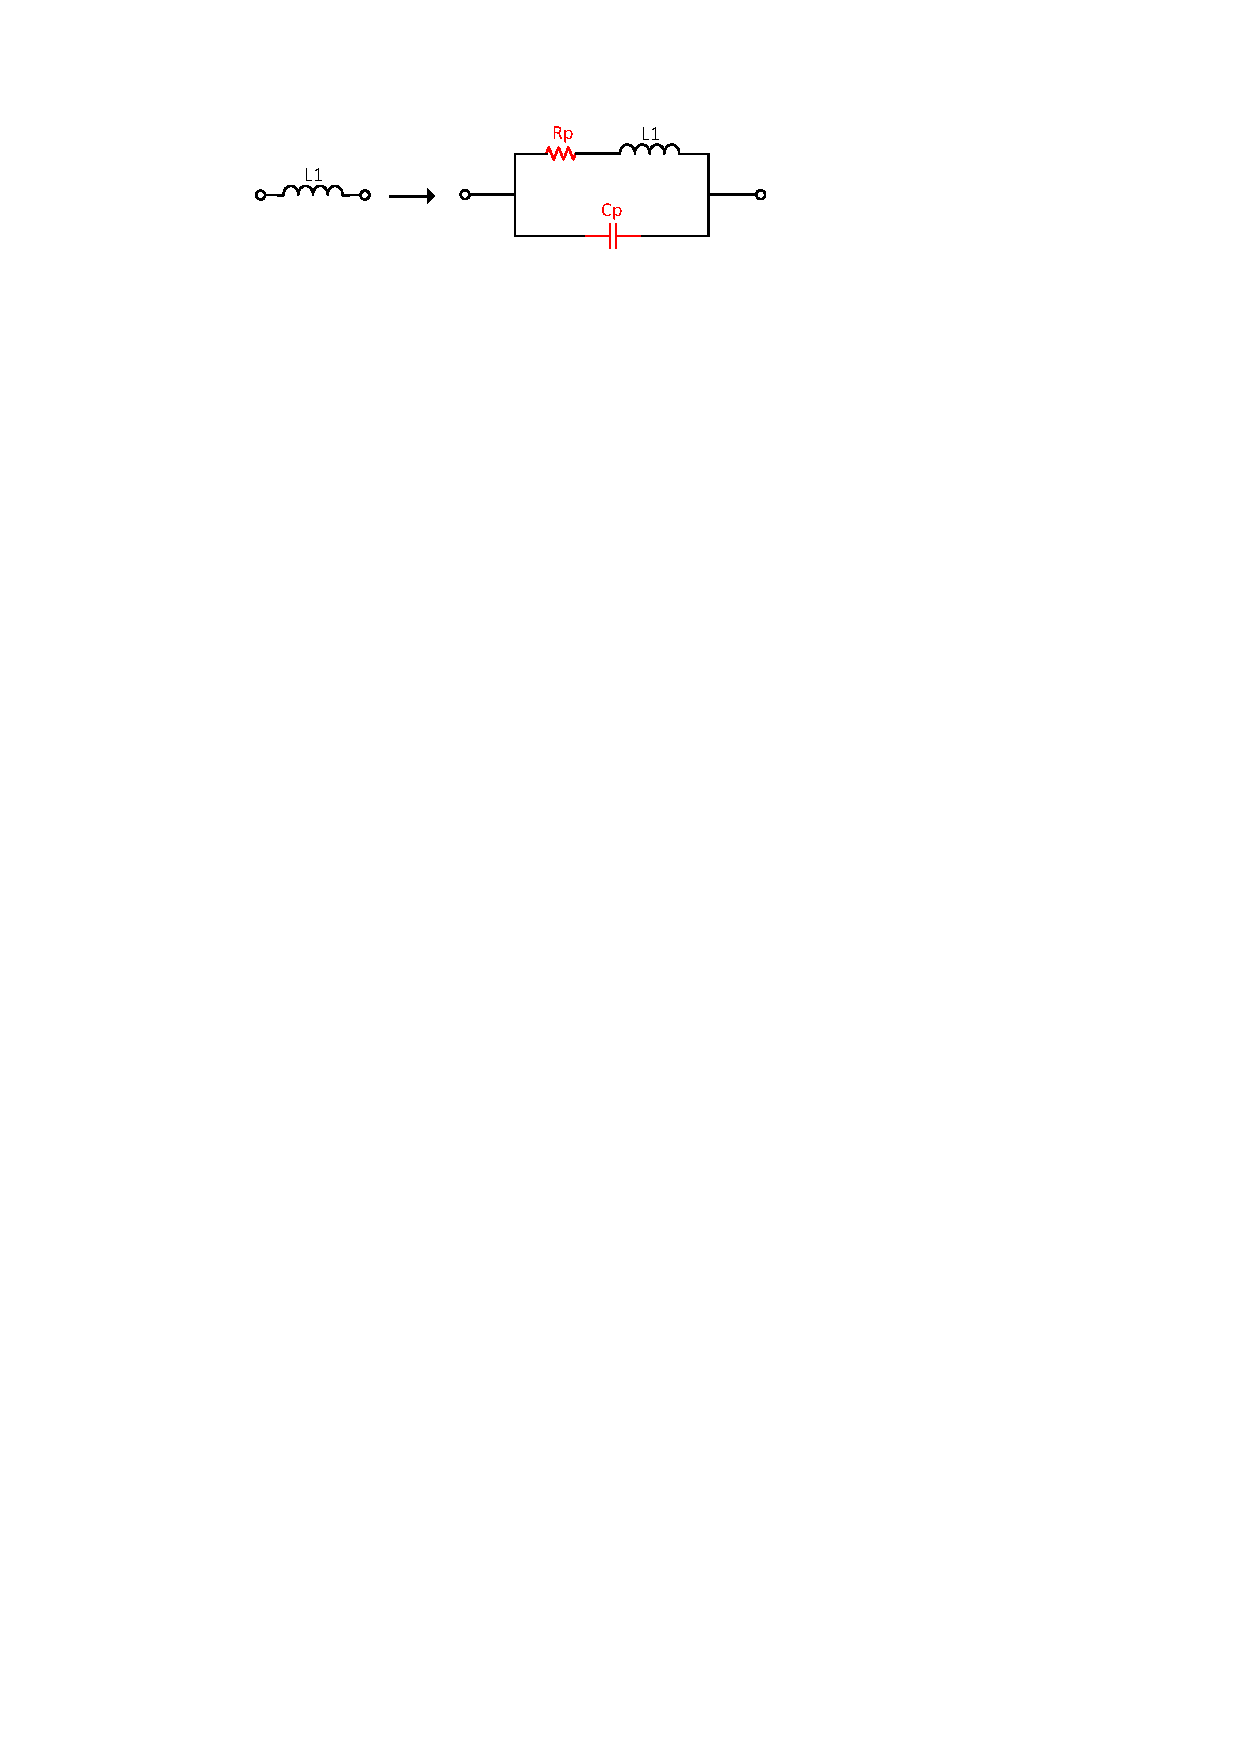
\includegraphics[width=0.9\textwidth]{img/ant_non_ideal.pdf} 
   \caption{Real antenna model}
   \label{fig:ant_non_ideal}
\end{figure}

\begin{equation} \label{eq:quality_f} % quality factor
Q = \frac {\omega L}{R_{p}}
\end{equation}

\begin{equation} \label{eq:srf}	%SRF
SRF = \frac{1} {2\pi\sqrt{LC_{p}}}
\end{equation}\\

For purpose of this work, with provided dimensions of the antenna, it is first modelled in HFSS as shown in 
figure \ref{fig:ant_single_model} and its equivalent lumped circuit in figure \ref{fig:ant_single_schematic}. It is important to 
note here that L1 in \ref{fig:ant_single_schematic} is in fact \ref{fig:ant_non_ideal}. However, in the discussion ahead, these 
parasitics are not explicitly mentioned for the sake of simplicity because the parameter extraction will include these factors too and on the other hand the operating frequency here is much less than coil SRF. To realise a real antenna, physical parameters of materials used for making 
printed antenna on a PCB are also given for the model.  After completing model, frequency sweep is done for extracting S parameter of the 
antenna which was eventually used to estimate  self inductance of the modelled coil. The performance estimation of 
single antenna here and couple system later is based on formulas in \cite{ant_SZ_formula}. In order to check and compare the estimated inductance value from 
the model, Modified Wheeler Formula, a mathematical approximation model described in \cite{ant_inductance_calculation} is used. The 
qualities of antenna obtained from extracted S-parameter are listed in table \ref{tab:ant_inductance_compare}. The table shows that 
modelled inductance value is less than mathematically approximated value. This difference can be explained with two things. 
Firstly, mathematical calculation assumed that the antenna is spiral and rectangular with sharp edge but the model has 
rounded edge. Secondly, during modelling besides dimensions of the coils, physical parameters of coil materials are also used 
but these are not considered for mathematical calculation.\\

\begin{figure} [!htbp]
  \centering 
  \subfloat[HFSS antenna model]  {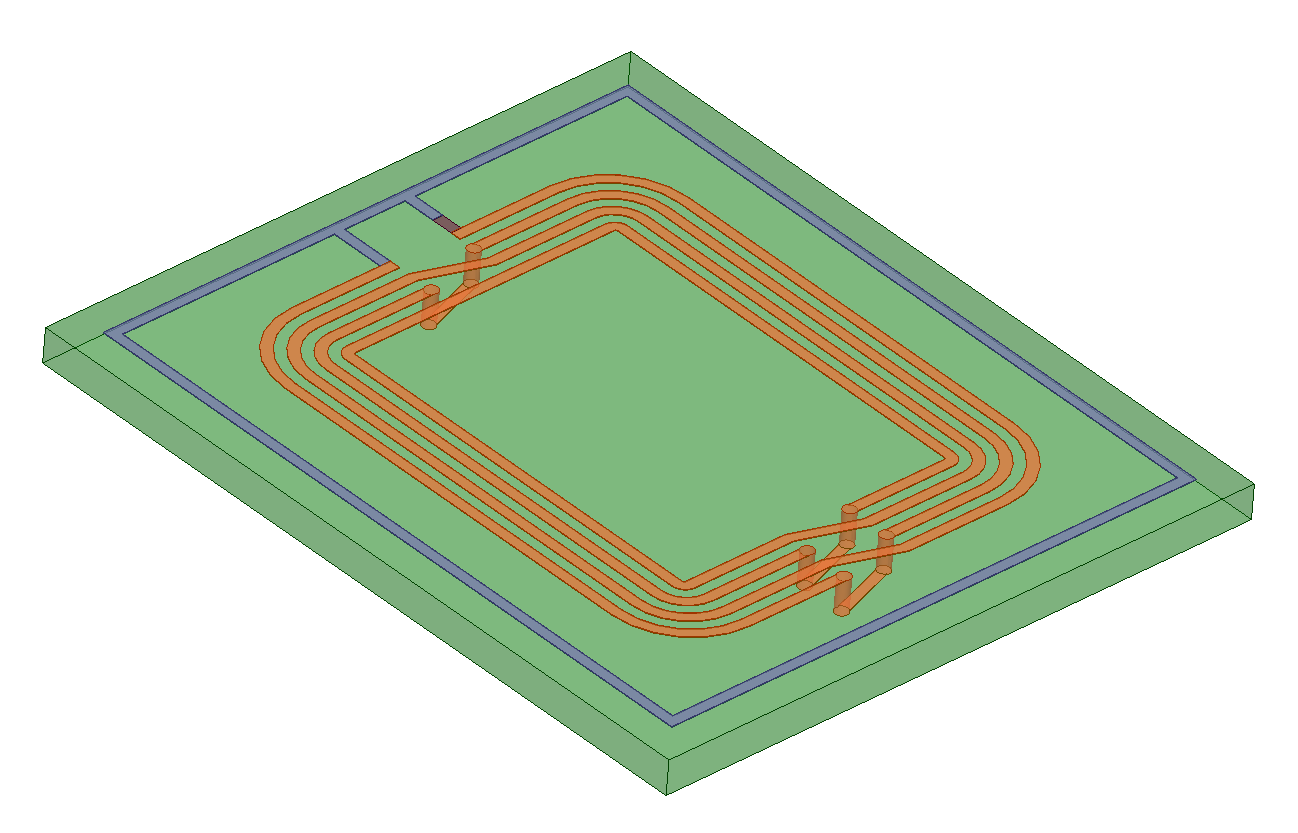
\includegraphics[width=.49\textwidth]{img/ant_single.png} \label{fig:ant_single_model}}
\hfill
 \subfloat[Equivalent schematic]  {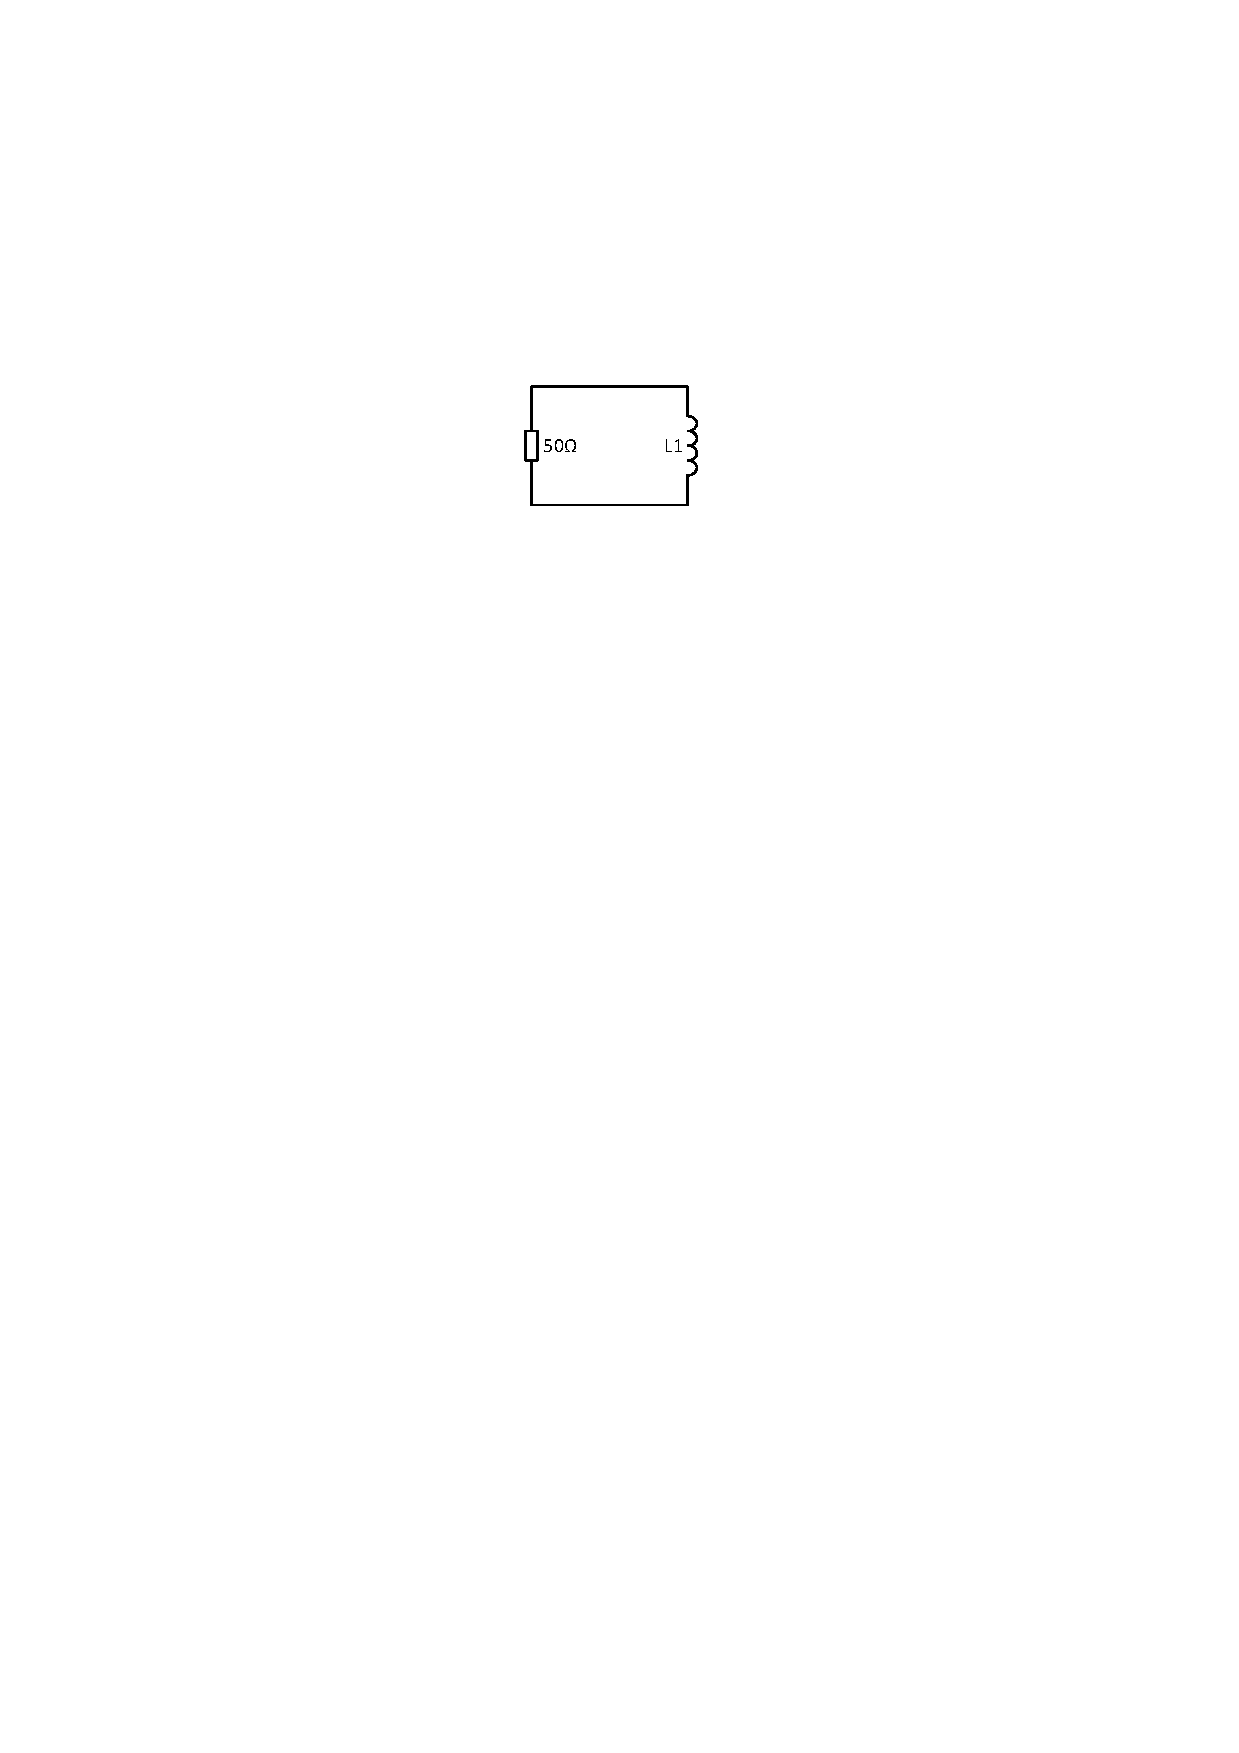
\includegraphics[width=.49\textwidth]{img/ant_single.pdf}\label{fig:ant_single_schematic}}
 \caption{Antenna model} 
\label{fig:ant_single} 
\end{figure}

\begin{table}[!htbp]
\caption{Characterisation of antenna} 
\begin{center}
\begin{tabular}{c|c|c}
\hline \hline
			& HFSS model 			& Modified Wheeler \cite{ant_inductance_calculation}  \\ \hline \hline
Self Inductance	  	& 448 \si{\nano\henry} 		& 644 \si{\nano\henry} \\ \hline
SRF		  	& 125 MHz			& 			\\ \hline
Quality factor		& 				&			\\ \hline
Parasitic Resistance	&				&			\\ \hline
Parasitic Capacitancce  &				&			\\	  
\hline \hline
\end{tabular}
\end{center}
\label{tab:ant_inductance_compare}
\end{table}%

\section{Inductive transfer link}		%****************************

In the next step, an inductive link is realised by using two antennas: one as primary and other as secondary, aligned one over 
other and separated by air gap as shown in figure  \ref{fig:ant_couple_model}, equivalently shown as lumped schematic in 
figure  \ref{fig:ant_couple_schematic}. Coupling system of these antennas is simulated for 
varying distance of magnetic field interaction to observe the difference in performance. The same procedure as 
used for single coil above, is used to extract self inductance of each coil, $L1$ and $L2$, mutual inductance 
of two coils, $L12$, coupling coefficient between the coils, $k$ and quality factor, $Q$. The extracted values for coil separation of 
1mm, 5mm and 10mm are listed in table \ref{tab:ant_couple_parameter} calculated at operating frequency of 13.56 MHz. \\

\begin{figure} [htbp]
  \centering 
  \subfloat[HFSS coupling model]  {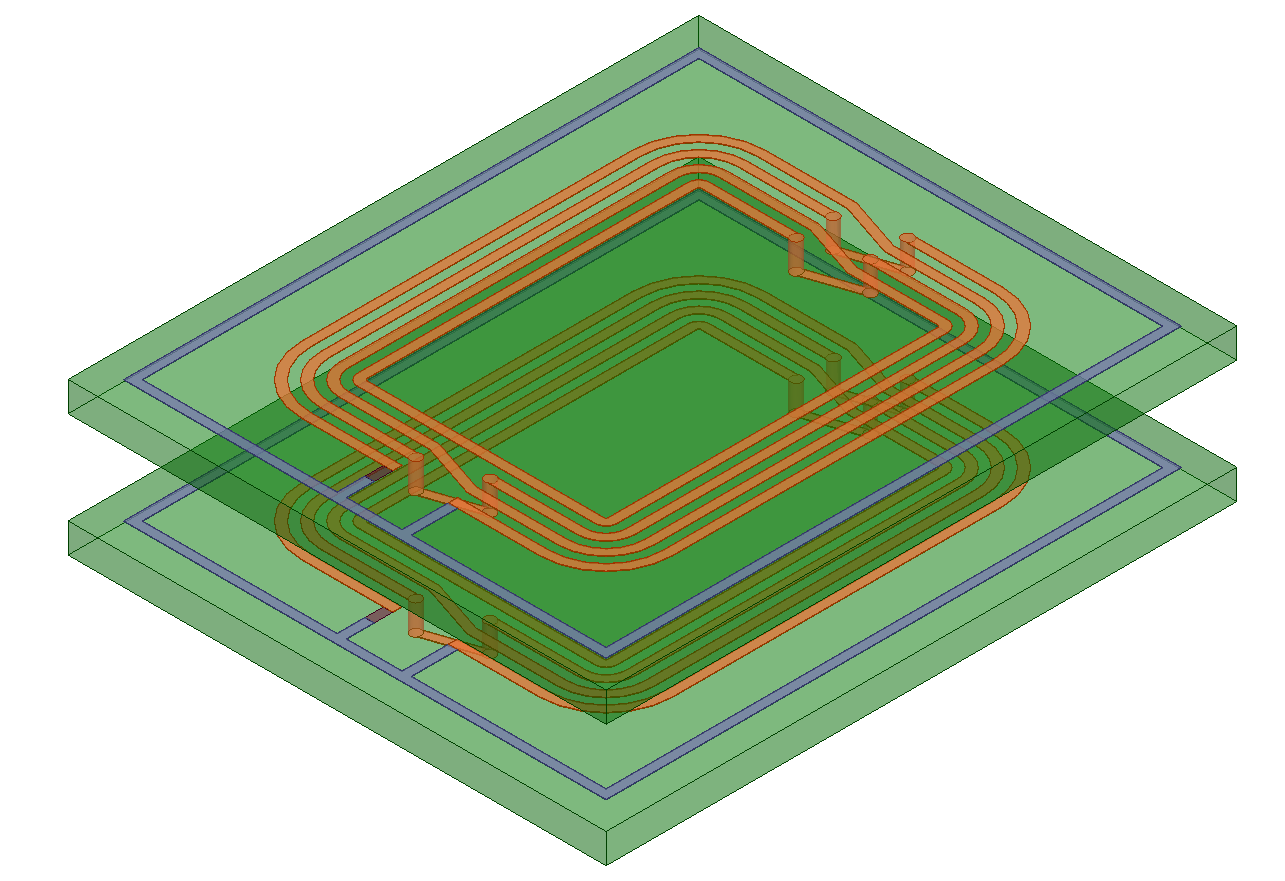
\includegraphics[width=.49\textwidth]{img/ant_couple.png} \label{fig:ant_couple_model}}
\hfill
 \subfloat[Equivalent schematic]  {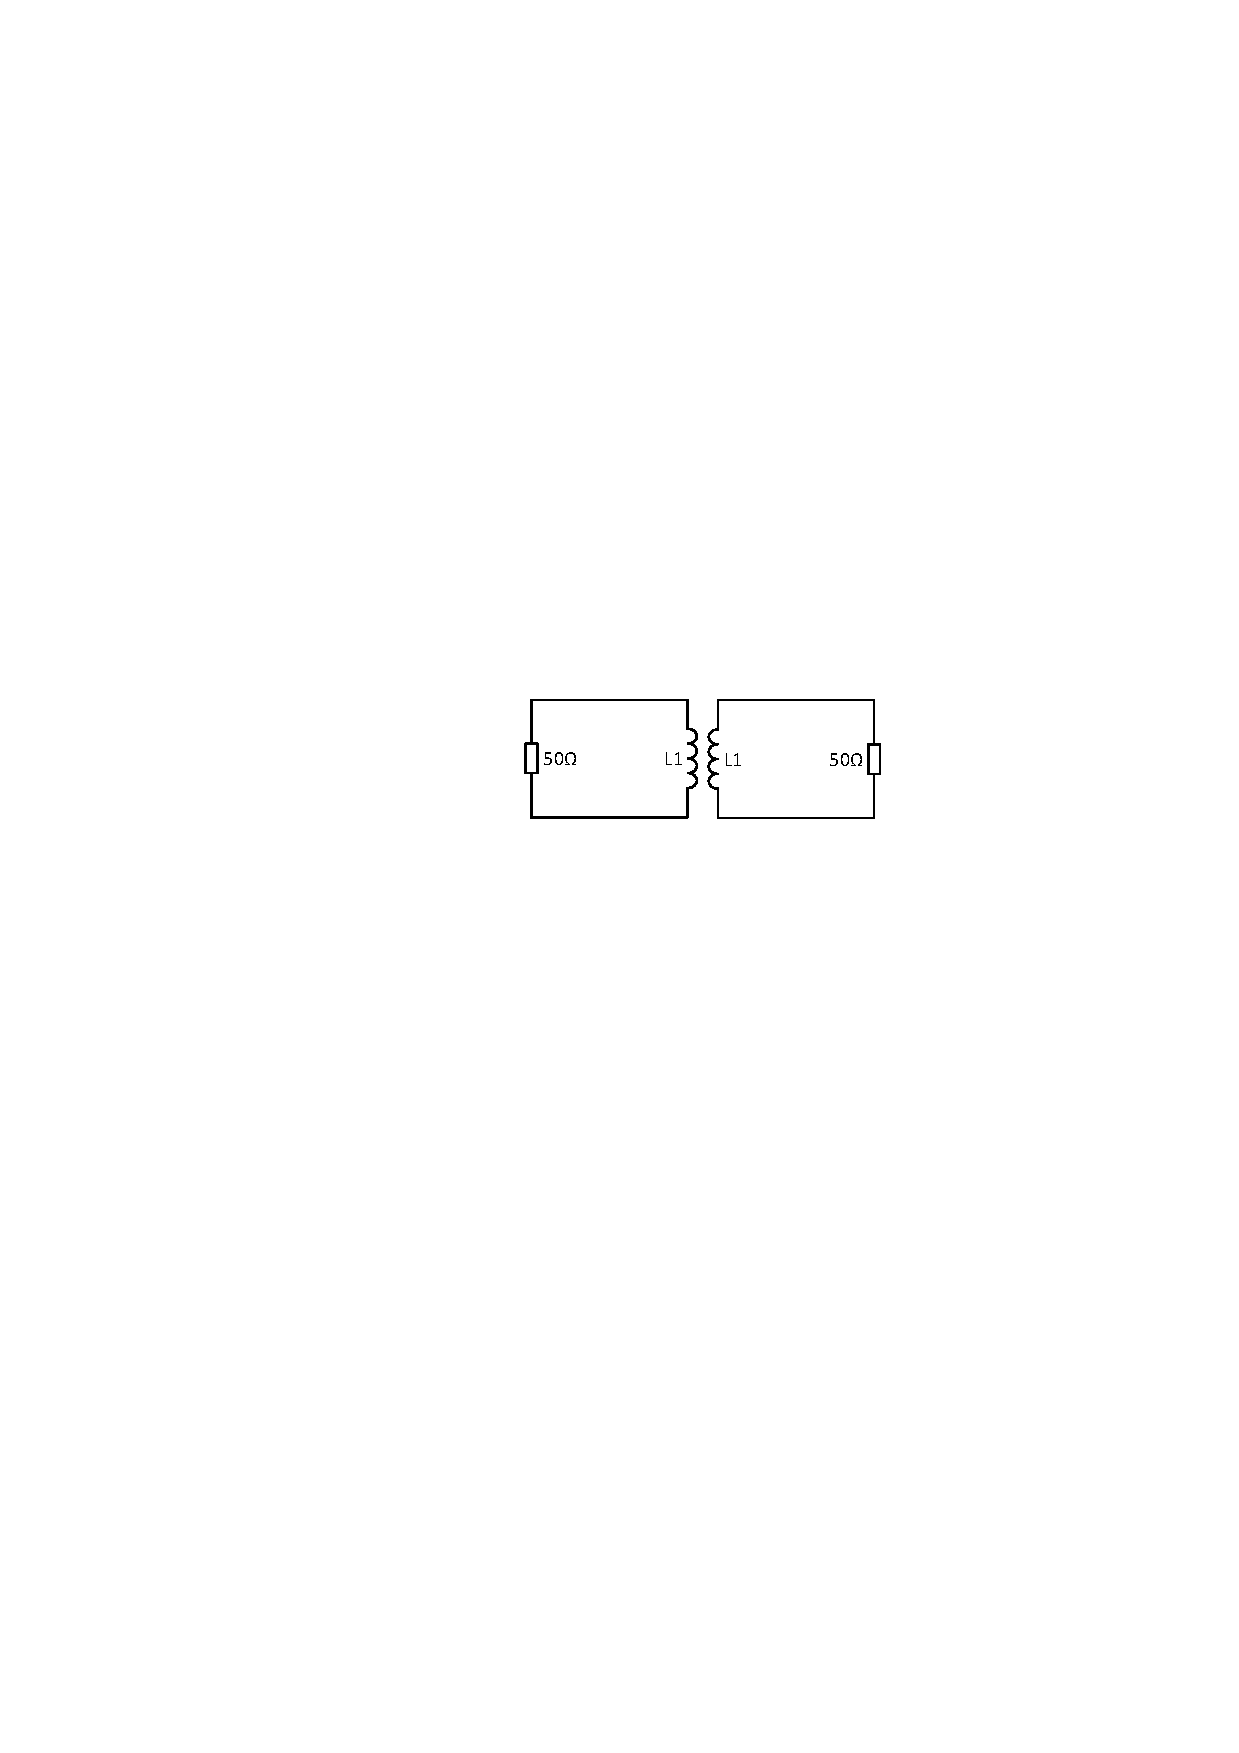
\includegraphics[width=.49\textwidth]{img/ant_couple.pdf}\label{fig:ant_couple_schematic}}
 \caption{Antenna coupling model} 
\label{fig:ant_couple} 
\end{figure}

\begin{table}[H]
\caption{Coupling parameters for varying coils distance} 
\begin{center}
\begin{tabular}{c|c|c|c|c}
\hline \hline
Parameter 	& 1 mm	& 5 mm 	& 10 mm	 & \si{\milli\meter}\\ \hline
L1		& -	& -	& -	 & \si{\nano\henry} \\ \hline
L2		& -	& -	& -	 & \si{\nano\henry} \\ \hline
L12		& -	& -	& -	 & \si{\nano\henry} \\ \hline
k		& -	& -	& -	 & -		    \\ \hline
Q		& -	& -	& -	 & -		    \\	\hline
SRF		&	&	&	 &		\\
\hline \hline
\end{tabular}
\end{center}
\label{tab:ant_couple_parameter}
\end{table}%

It is observed that $L1$ and $L2$ are same as in table \ref{tab:ant_inductance_compare} as it is the same coil used as primary 
and secondary. Similarly $L12$ and $k$, related as $L12 = k\sqrt(L1L2)$, are both decreasing with distance as expected. With 
increase in separation, less and less magnetic flux generated by primary coil is linked with the secondary, creating a loosley
coupled inductive link. \\

As already stated, power transfer efficiency depends on k of coupling system and Q of coils and hence high k and high Q is always desirable and obviously 
coil optimisation is the most important part of coupling system design. \cite{ant_optimal_resonance} and \cite{ant_PSC_geometry} 
discusses some techniques to optimise transfer efficiency of inductive link: \cite{ant_optimal_resonance} about matching the 
load for better resonance whereas \cite{ant_PSC_geometry} about designing optimal coil geometry for higher Q. The former one 
compares the efficiency of general inductive coupling and conventional resonant coupling and their limitation in achieving 
higher efficiency. This eventually proposes optimal resonant load transformation which has better immunity to poor coupling 
and load variation. Likewise, the later one describes step by step iterative process of designing an antenna with optimal geometry for the given 
design constraints. \\

\section{Magnetic resonance coupling}  	%****************************

In this project, conventional magnetic resonance coupling as in is implemented to tune both primary and secondary 
at same frequency. The purpose here is to tune the secondary antenna of 
coupling system to the operating frequency to cancel the leakage inductance and increase quality factor, and tune the primary antenna to the same frequency to increase the 
driving current. Thus creating resonance in an inductive link maximise the power transmission from the source to  the load.  \\


For the purpose of making a resonant inductive link, the S parameter of coupled antenna system in HFSS 
is exported to ADS in order to design matching networks using capacitors only. Impedance of  primary antenna is 
matched to 50 \si{\ohm} source resistance and impedance of secondary is matched to load impedance (50 \si{\ohm} load or input 
impedance chip(?)) as shown in \ref{fig:ant_couple_resonant}. $Cp1$, series capacitor and $Cp2$, shunt capacitor together 
with $L1$ created parallel resonant circuit at 13.56 MHz on the primary side and $Cs1$, shunt capacitor together with $L2$ 
creates the secondary resonant circuit at same operating frequency. Thus a pair of LC tank circuit is made tuned at same 
frequency. Such matching network is designed for all three coil separation distances as above, but resonant coupling system 
with 5 mm separation is taken as a typical example and presented here. \\

The reflection power loss, S11 and S22, at both primary and secondary terminal, power transfer gain, S21, from primary 
to secondary and Q-factors for both antennas before and after creating resonance are shown in figure \ref{fig:ant_S_loss}, 
this and this. \\

\begin{figure}[!htbp] %figure placement: here, top, bottom, or page
   \centering
   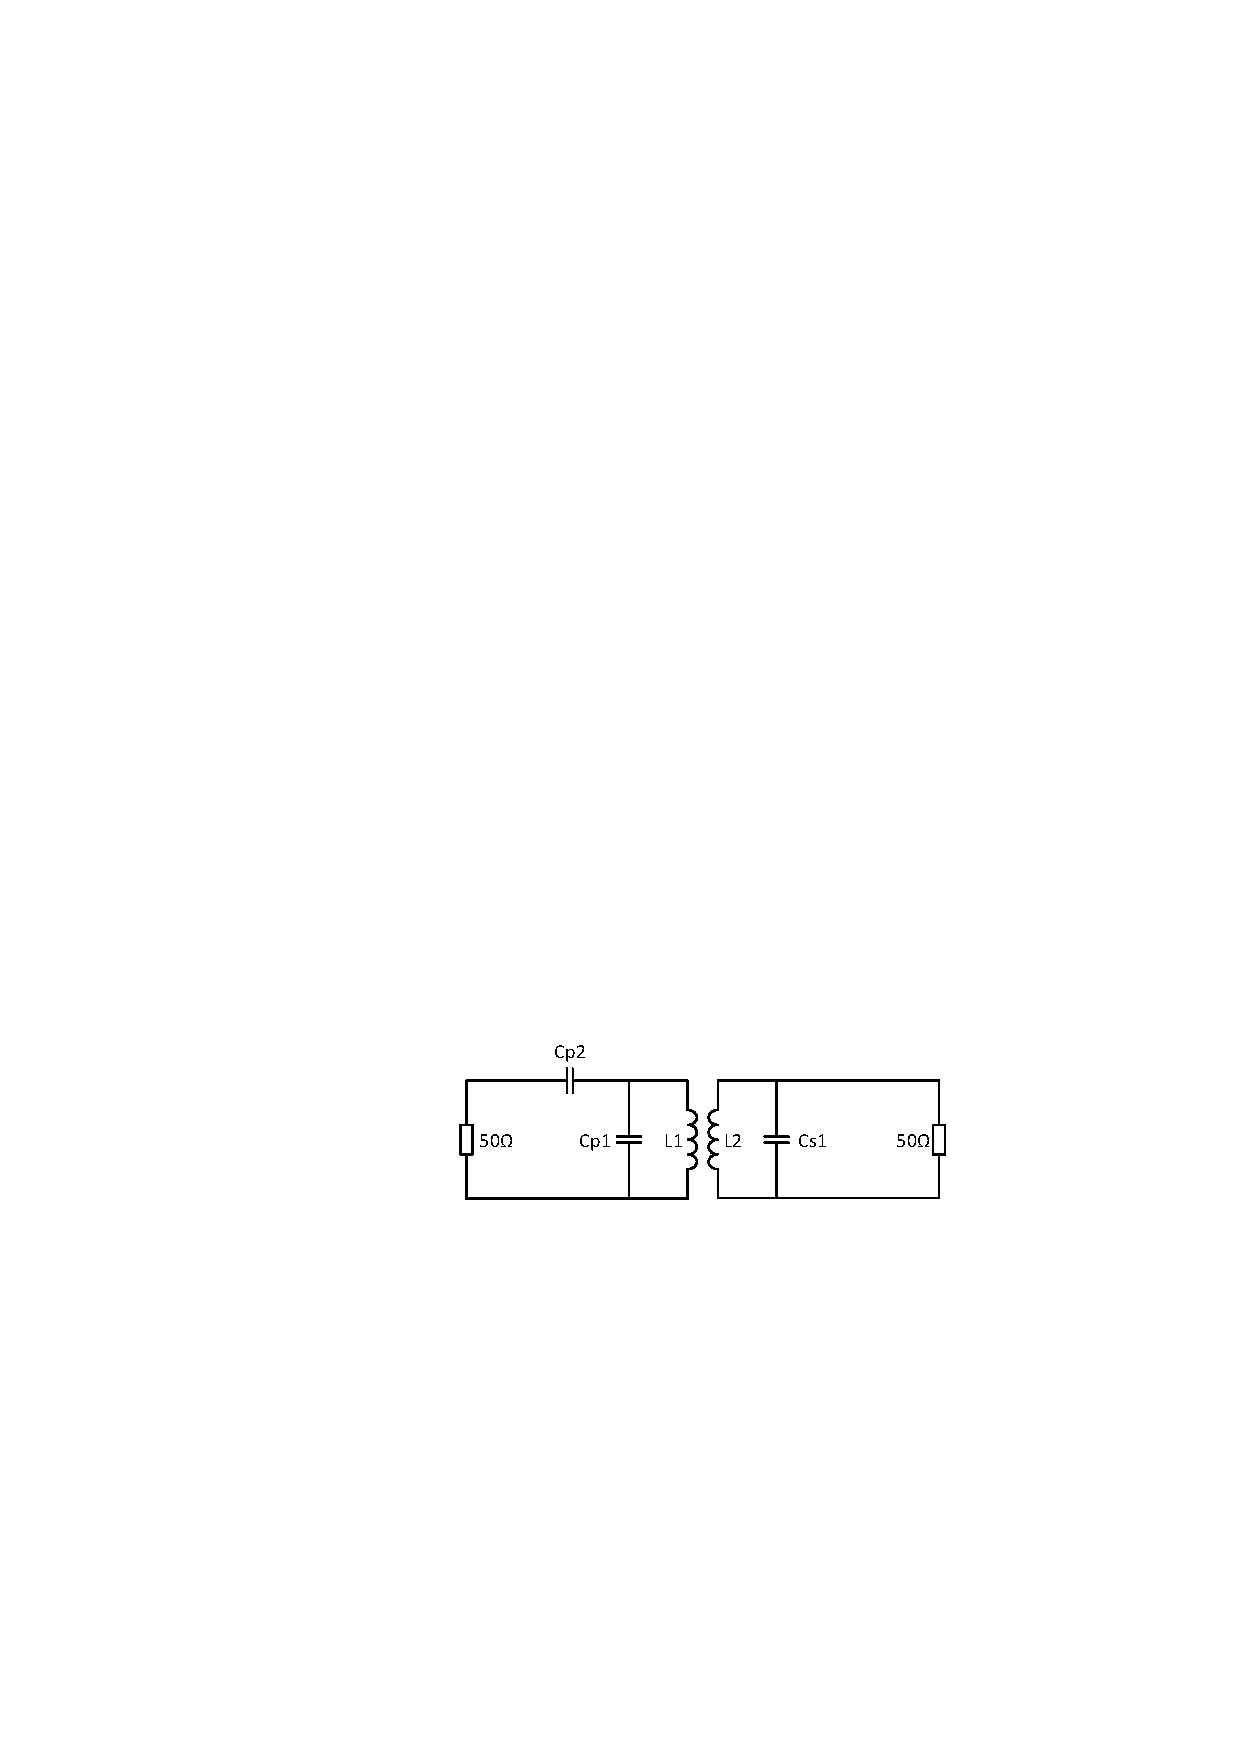
\includegraphics[width=0.8\textwidth]{img/ant_couple_resonant.pdf} 
   \caption{Resonant coupled inductive link}
   \label{fig:ant_couple_resonant}
\end{figure}

\begin{figure} [!htbp]
  \centering
  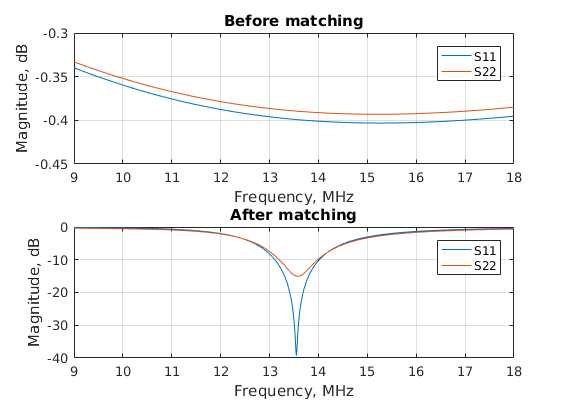
\includegraphics[width=0.9\textwidth]{img/ant_S_loss.png} 
 \caption{Power loss before and after matching} 
\label{fig:ant_S_loss} 
\end{figure}

The performance of magnetic resonant coupling link designed in this work is summarises in table \ref{tab:ant_spec} below.

\begin{table}[!htbp]
\caption{Performance of resonant inductive link} 
\begin{center}
\begin{tabular}{c|c}
\hline \hline
$Cp1$ $Cp2$ and $Cs1$	  	& 			\\ \hline
Resonant frequency		& 13.56 MHz		\\ \hline
Primary reflection loss		&			\\ \hline
Secondary reflection loss	& 			\\ \hline
Primary to secondary gaining	& 			\\ \hline
Q-factor			&			\\
\hline \hline
\end{tabular}
\end{center}
\label{tab:ant_spec}
\end{table}%

\clearpage
\newpage

% *********************************************************************** WPT PRU SYSTEM  ***********************************************************************************

\part{WPT System Design and Implementation}      

\chapter{Power Receiving Unit Design} 

\section{Introduction}		%****************************

Wireless power transfer, \acrshort{wpt} system always constitutes two main units: power transmitting unit, 
\acrshort{ptu} and power receiving unit, \acrshort{pru}. Each unit comprises of resonator, power conditioner 
and control circuits as shown in figure \ref{fig:wpt_ptu_pru}. Both the resonators in PRU and PTU are tuned to operating 
frequency, which create a physical transfer link. Power conditioner circuit in PTU includes at least power 
amplifier and matching circuit, whereas in PRU, it includes matching circuit, rectifier and regulator. 
Similarly both these units have control block which facilitates transfer procedure and communication between 
these units.  In this work, design and analysis of PRU is the main objective.  \\
%Since PRU cannot be realised without a transfer link, primary antenna creates a very simply PTU here.  \\

\begin{figure} 
  \centering
  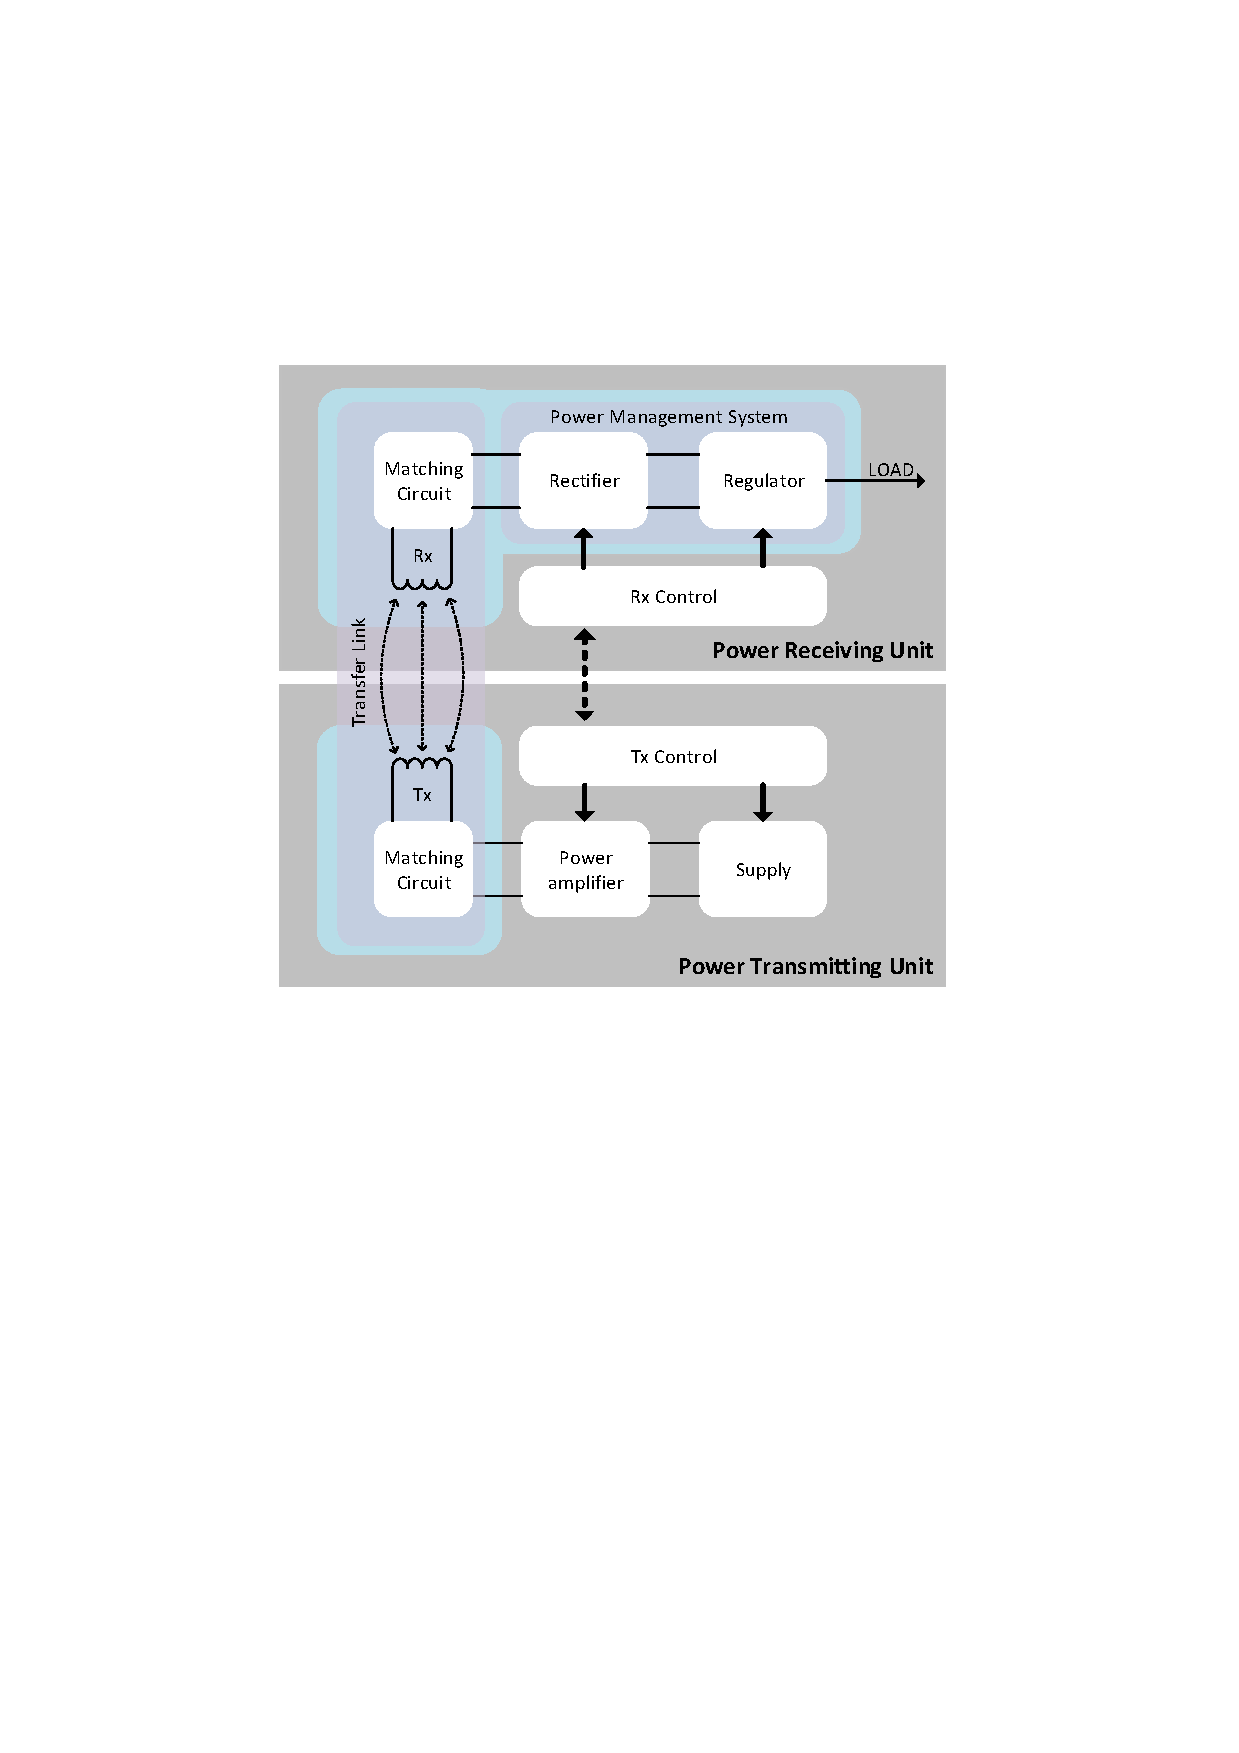
\includegraphics[width=0.9\textwidth]{img/wpt_ptu_pru.pdf} 
 \caption{WPT block diagram} 
\label{fig:wpt_ptu_pru} 
\end{figure}


In figure \ref{fig:wpt_ptu_pru} above, the block highlighted in blue is the PRU system in this design. Secondary coil, Rx is the receiver resonator, and  
rectifier and regulator is power conditioning block. The primary coil is driven by a power source and AC signal is generated at the secondary as discussed 
earlier in antenna design section. The rectifier then rectifies this AC signal to DC. The DC output of the rectifier is then fed to LDO 
to produce regulated DC output required to drive a load. The reference and biasing circuit generates required reference and biasing DC voltages for the LDO. \\

The PRU unit is broken down into two sub units for step wise analysis. As seen in the block diagram, it is functionally divided into Transfer Link and 
Power Management System (\acrshort{pms}). Firstly, PMS is simulated excluding the transfer link to characterise the performance of PMS. Secondly, the whole PRU system: PMS with transfer link created with coupled antenna, Tx and Rx, is simulated to observe the performance of whole PRU. Though it has already been told earlier, 
one important thing must be mentioned here again before going further. Even though reference and biasing circuit has 
been integrated into the PMS system, it has been designed with an option to override it externally. This externally 
supplied reference and biasing will be primarily used for the PRU system simulation. The result with on-system biases 
and reference will be explicitly noted when used. \\

\section{Power Management System}

Figure \ref{fig:wpt_top} is the top level of PMS in this design and test bench setup is a shown in figure \ref{fig:wpt_top_testbench}. The purpose here is to give differential signal Vin1 and Vin2 from source Vac and see Vrec and Vreg outputs while driving maximum load. The other inputs are external biases, reference, control and supply for LDO and buffer. Other outputs are biases voltages to examine the performance of BGR circuit which is disabled now with external control signal Vctl low.  \\

\begin{figure} [!htbp]
  \centering
  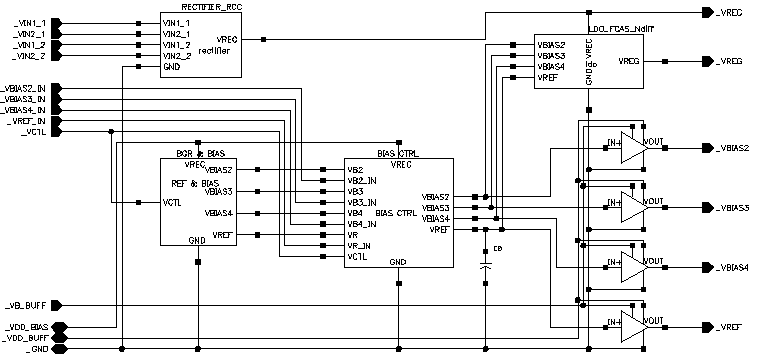
\includegraphics[width=\textwidth]{img/wpt_top.pdf} 
 \caption{WPT PMS implementation} 
\label{fig:wpt_top} 
\end{figure}

\vspace{5mm}

\begin{figure} [H]
  \centering
  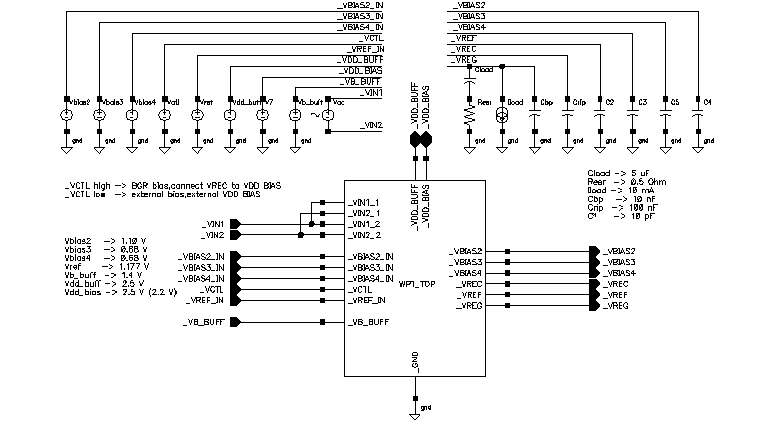
\includegraphics[width=\textwidth]{img/wpt_top_testbench.pdf} 
 \caption{Test bench for PMS simulation } 
\label{fig:wpt_top_testbench} 
\end{figure}

\subsection{Transient Response}

\begin{figure} [H]
  \centering
  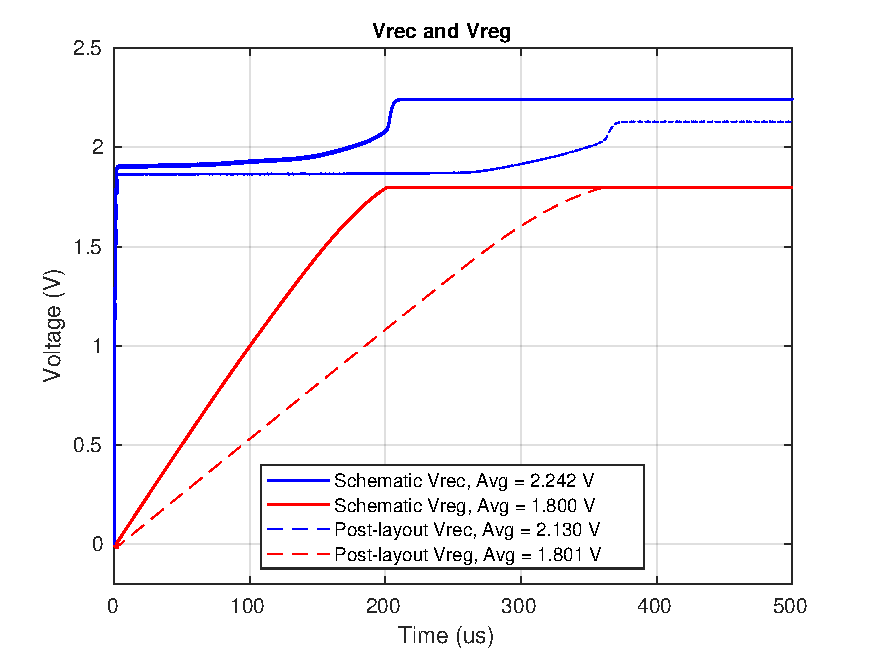
\includegraphics[width=\textwidth]{img/wpt_V_wo_bgr_both.pdf} 
 \caption{Transient Vrec and Vreg} 
\label{fig:wpt_V_wo} 
\end{figure}

\begin{figure} [H]
  \centering
  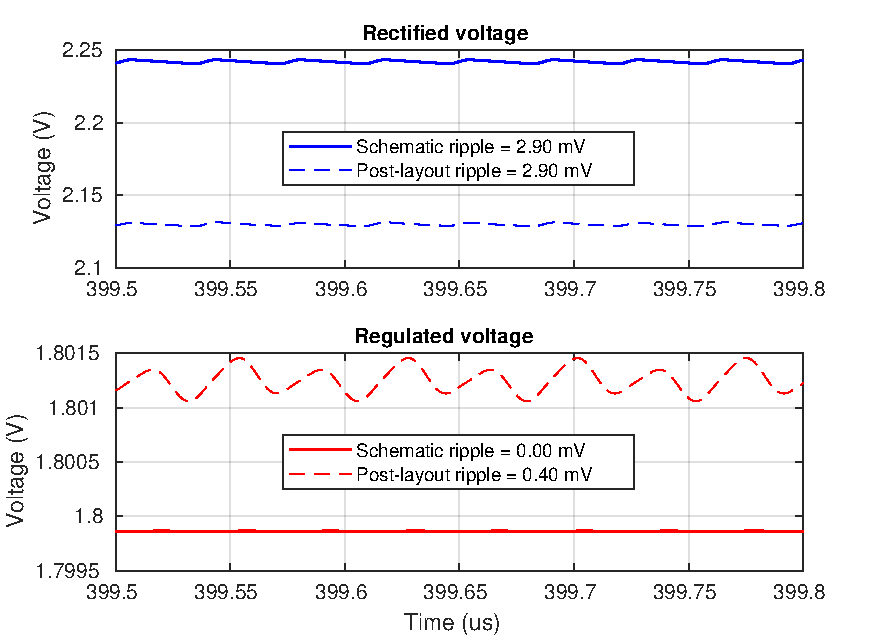
\includegraphics[width=\textwidth]{img/wpt_ripple_wo_bgr_both.pdf} 
 \caption{Ripple in Vrec and Vreg} 
\label{fig:wpt_ripple_wo} 
\end{figure}


\section{PRU Unit}

Figure \ref{fig:wpt_top_link} is test bench for complete PRU unit. It includes PMS shown in figure \ref{fig:wpt_top} and resonant inductive link shown in figure \ref{fig:ant_couple}. This inductive link is coupling model extracted from HFSS and both antennas tuned at the operating frequency, 13.56 MHz. The primary antenna is driven by signal source Vac and the secondary antenna generate differential signal Vin1 and Vin2, the inputs for the chip. Other biasing voltages and componoent values remain the same as in PMS simulation. \\

\begin{figure} [H]
  \centering
  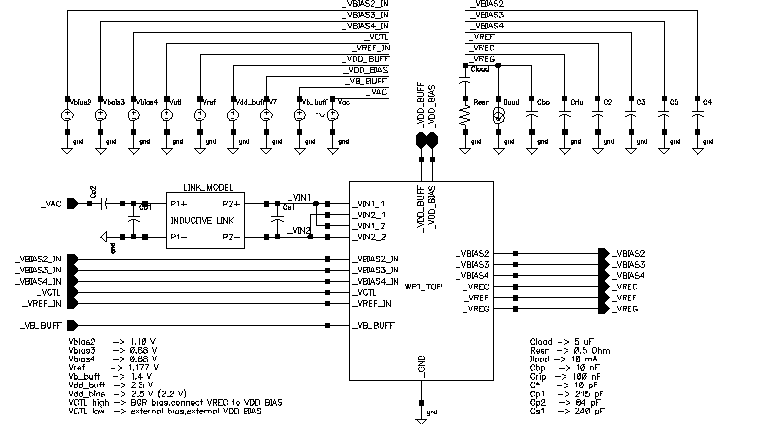
\includegraphics[width=\textwidth]{img/wpt_top_link.pdf} 
 \caption{Test bench for complete PRU unit } 
\label{fig:wpt_top_link} 
\end{figure}

The parasitic extraction of the compete layout also includes the tracks from pad to core inputs. The pad-frame layout provided by the fab was used to accurately draw the tracks from pad to core I/O terminals. \\


\chapter{Chip Production, Test and Verification}

\section{Chip and PCB}
After post layout simulation of complete PRU system, it was sent for production to TSMC fab in November 2016 and was received in February 2017. The  manufactured chip was packaged in 84 I/O pins \acrshort{jlcc} package. The full layout is included in appendix *. It is designed in 90nm process using 2.5 V devices. This process provides 1P-9M - 1 poly layer and 9 metal layers. However in this design, 1 poly and 8 metal layers is used. Basically every component layout used up-to 4 metal layers. Only the high current paths are made with parallel path of higher metal layers. The micrograph of produced layout is shown in figure [CHIP MICRO PCITURE] .\\

While the chip was in production, test PCB board and antennas were designed and produced. EAGLE is used as PCB design tool. Jumper header pins are used for DC voltages whereas for ac inputs SMA connectors are used. Similarly, for decoupling and ripple rejection \acrshort{smd} \acrshort{mlcc} capacitors are used but  for stability purpose of LDO, electrolytic capacitor is used owing to requirement of better accuracy and higher ESR for compensation capacitor.  In order to have better control of supplies to bias, buffer and pad circuits on board regulator is used. For convenience, instead of providing biases voltages from power supply, on board resistive network is implemented to generate required bias voltages. For sanity check of the chip, balun is used to created differential signal inputs. The test PCB and antenna are shown in figure [figure].\\


% ***********************************************************************  CONCLUSION ***********************************************************************************
\part{Conclusion}
\chapter{Conclusion}
\section{Problem and challenges}
\section{Future Work}

\clearpage
\newpage
\nocite{*}
\printbibliography

%\newpage
%\listoffigures
%\newpage
%\listoftables
%\printindex
\newpage
\printnoidxglossaries
\backmatter{}
\end{document}